%!TEX root = ../dissertation.tex
\chapter{Boosted singal region kinematic distributions}
\label{AppendixSR}

\paragraph{}
This appendix shows unblinded data with the prediction of QCD multi-jets and \ttbar~ backgrounds in the signal region. Plots shown are with stat uncertainty only.

\paragraph{}
Tables~\ref{tab:sr-region-4b}, ~\ref{tab:sr-region-3b}, ~\ref{tab:sr-region-2b}, ~\ref{tab:sr-region-4b-pole}, ~\ref{tab:sr-region-3b-pole}, ~\ref{tab:sr-region-2b-pole} shows the integrated SR predictions and yields, in different \mtwoJ or scaled \mtwoJ ranges. The predictions agree with the data fairly well, with the exception of the $3b$ deficient in \mtwoJ above $2$ \TeV.

\begin{table}[htbp!]
\scriptsize
\begin{center}
\begin{footnotesize} 
\begin{tabular}{c|c|c|c|c|c} 
Mass Range & >1000 & >1500 & >2000 & >2500 & >3000 \\ 
\hline\hline 
totalbkg & 23.09 $\pm$ 1.59 & 1.94 $\pm$ 0.15 & 0.26 $\pm$ 0.072 & 0.061 $\pm$ 0.058 & 0.021 $\pm$ 0.047\\ 
data & 21.0 $\pm$ 4.58 & 3.0 $\pm$ 1.73 &  -  &  -  &  - \\ 
\hline\hline 
\end{tabular} 
\end{footnotesize} 
\newline 

\caption{$4b$ unblinded signal region predictions and results. All systematic uncertainties included for backgrounds. For Data, the statistical uncertainty is shown. Mass range is broken into greater than 1 TeV, 1.5 TeV, 2 TeV, 2.5 TeV, and 3 TeV intervals.}
\label{tab:sr-region-4b}
\end{center}
\end{table}

\begin{table}[htbp!]
\scriptsize
\begin{center}
\begin{footnotesize} 
\begin{tabular}{c|c|c|c|c|c} 
Mass Range & >1000 & >1500 & >2000 & >2500 & >3000 \\ 
\hline\hline 
totalbkg & 495.92 $\pm$ 12.34 & 51.72 $\pm$ 2.46 & 10.42 $\pm$ 0.95 & 4.07 $\pm$ 0.85 & 2.21 $\pm$ 0.79\\ 
data & 499.0 $\pm$ 22.34 & 42.0 $\pm$ 6.48 & 3.0 $\pm$ 1.73 & 1.0 $\pm$ 1.0 &  - \\ 
\hline\hline 
\end{tabular} 
\end{footnotesize} 
\newline 

\caption{$3b$ unblinded signal region predictions and results. All systematic uncertainties included for backgrounds. For Data, the statistical uncertainty is shown. Mass range is broken into greater than 1 TeV, 1.5 TeV, 2 TeV, 2.5 TeV, and 3 TeV intervals.}
\label{tab:sr-region-3b}
\end{center}
\end{table}

\begin{table}[htbp!]
\scriptsize
\begin{center}
\begin{footnotesize} 
\begin{tabular}{c|c|c|c|c|c} 
Mass Range & >1000 & >1500 & >2000 & >2500 & >3000 \\ 
\hline\hline 
totalbkg & 2688.71 $\pm$ 34.09 & 288.51 $\pm$ 4.96 & 42.19 $\pm$ 2.13 & 8.85 $\pm$ 1.55 & 2.72 $\pm$ 1.09\\ 
data & 2755.0 $\pm$ 52.49 & 287.0 $\pm$ 16.94 & 38.0 $\pm$ 6.16 & 4.0 $\pm$ 2.0 & 1.0 $\pm$ 1.0\\ 
\hline\hline 
\end{tabular} 
\end{footnotesize} 
\newline 

\caption{$2bs$ unblinded signal region predictions and results. All systematic uncertainties included for backgrounds. For Data, the statistical uncertainty is shown. Mass range is broken into greater than 1 TeV, 1.5 TeV, 2 TeV, 2.5 TeV, and 3 TeV intervals.}
\label{tab:sr-region-2b}
\end{center}
\end{table}


\begin{table}[htbp!]
\scriptsize
\begin{center}
\begin{footnotesize} 
\begin{tabular}{c|c|c|c|c|c} 
Mass Range & >1000 & >1500 & >2000 & >2500 & >3000 \\ 
\hline\hline 
totalbkg & 24.64 $\pm$ 1.84 & 2.84 $\pm$ 0.22 & 0.25 $\pm$ 0.044 & 0.02 $\pm$ 0.011 & 0.0014 $\pm$ 0.0026\\ 
data & 22.0 $\pm$ 4.69 & 4.0 $\pm$ 2.0 & 1.0 $\pm$ 1.0 &  -  &  - \\ 
\hline\hline 
\end{tabular} 
\end{footnotesize} 
\newline 

\caption{$4b$ unblinded scaled dijet mass signal region predictions and results. All systematic uncertainties included for backgrounds. For Data, the statistical uncertainty is shown. Mass range is broken into greater than 1 TeV, 1.5 TeV, 2 TeV, 2.5 TeV, and 3 TeV intervals.}
\label{tab:sr-region-4b-pole}
\end{center}
\end{table}

\begin{table}[htbp!]
\scriptsize
\begin{center}
\begin{footnotesize} 
\begin{tabular}{c|c|c|c|c|c} 
Mass Range & >1000 & >1500 & >2000 & >2500 & >3000 \\ 
\hline\hline 
totalbkg & 559.38 $\pm$ 14.06 & 69.27 $\pm$ 3.22 & 13.35 $\pm$ 1.14 & 4.37 $\pm$ 0.96 & 2.0 $\pm$ 0.87\\ 
data & 570.0 $\pm$ 23.87 & 59.0 $\pm$ 7.68 & 4.0 $\pm$ 2.0 & 1.0 $\pm$ 1.0 &  - \\ 
\hline\hline 
\end{tabular} 
\end{footnotesize} 
\newline 

\caption{$3b$ unblinded scaled dijet mass signal region predictions and results. All systematic uncertainties included for backgrounds. For Data, the statistical uncertainty is shown. Mass range is broken into greater than 1 TeV, 1.5 TeV, 2 TeV, 2.5 TeV, and 3 TeV intervals.}
\label{tab:sr-region-3b-pole}
\end{center}
\end{table}

\begin{table}[htbp!]
\scriptsize
\begin{center}
\begin{footnotesize} 
\begin{tabular}{c|c|c|c|c|c} 
Mass Range & >1000 & >1500 & >2000 & >2500 & >3000 \\ 
\hline\hline 
totalbkg & 2998.69 $\pm$ 40.31 & 377.8 $\pm$ 6.39 & 57.47 $\pm$ 2.88 & 11.78 $\pm$ 1.95 & 3.39 $\pm$ 1.27\\ 
data & 3078.0 $\pm$ 55.48 & 379.0 $\pm$ 19.47 & 47.0 $\pm$ 6.86 & 6.0 $\pm$ 2.45 & 2.0 $\pm$ 1.41\\ 
\hline\hline 
\end{tabular} 
\end{footnotesize} 
\newline 

\caption{$2bs$ unblinded scaled dijet mass signal region predictions and results. All systematic uncertainties included for backgrounds. For Data, the statistical uncertainty is shown. Mass range is broken into greater than 1 TeV, 1.5 TeV, 2 TeV, 2.5 TeV, and 3 TeV intervals.}
\label{tab:sr-region-2b-pole}
\end{center}
\end{table}

\paragraph{}
Figures~\ref{fig:boosted-4b-signal-ak10-lead}, \ref{fig:boosted-4b-signal-ak10-subl}, \ref{fig:boosted-4b-signal-ak2}, and \ref{fig:boosted-4b-signal-ak10-system} show predictions of various kinematics of the large-\R jets and their associated track jets in the $4b$ selection.
Figures~\ref{fig:boosted-3b-signal-ak10-lead}, \ref{fig:boosted-3b-signal-ak10-subl}, \ref{fig:boosted-3b-signal-ak2}, and \ref{fig:boosted-3b-signal-ak10-system} show predictions of various kinematics of the large-\R jets and their associated track jets in the $3b$ selection.
Figures~\ref{fig:boosted-2bs-signal-ak10-lead}, \ref{fig:boosted-2bs-signal-ak10-subl}, \ref{fig:boosted-2bs-signal-ak2}, and \ref{fig:boosted-2bs-signal-ak10-system} show predictions of various kinematics of the large-\R jets and their associated track jets in the $2b$ selection.

\begin{figure*}[htbp!]
\begin{center}
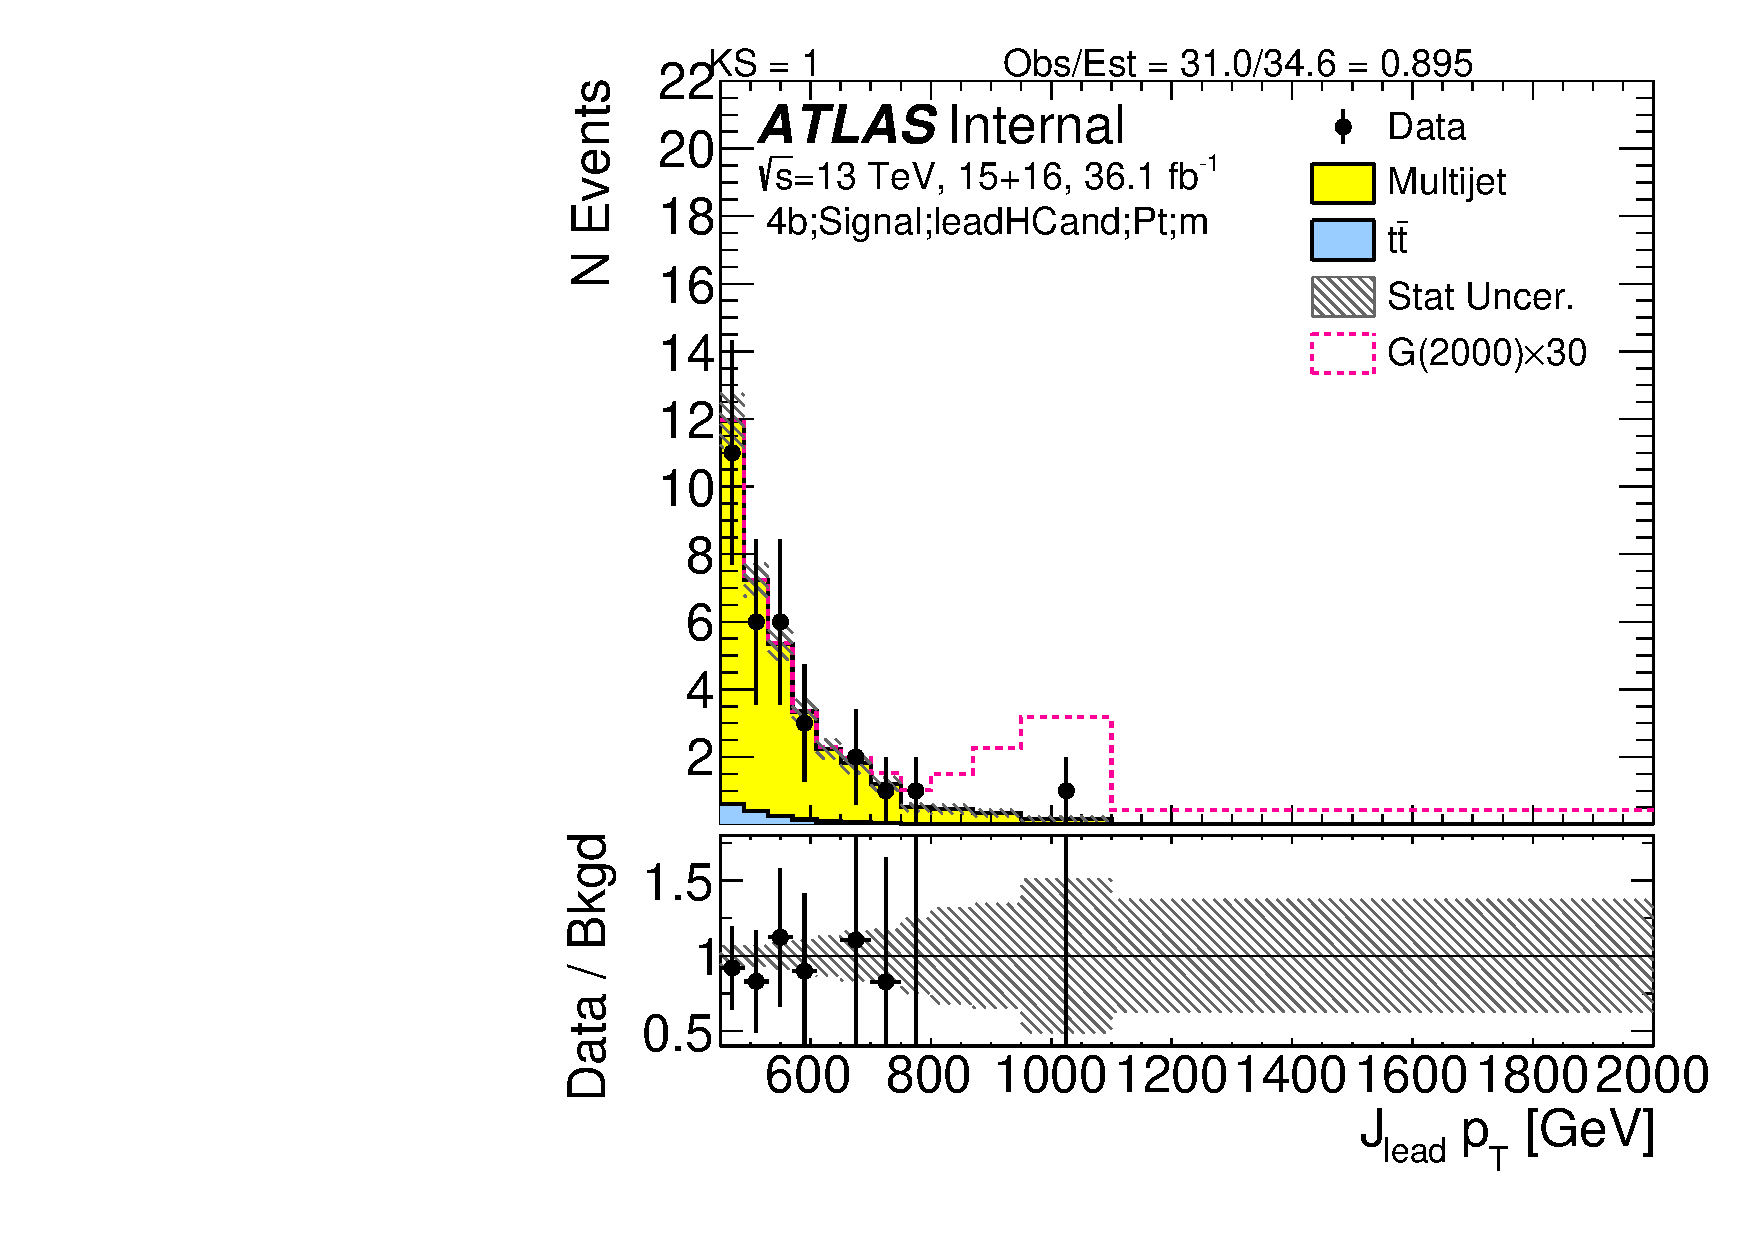
\includegraphics[width=0.31\textwidth,angle=-90]{figures/boosted/Signal/b77_FourTag_Signal_leadHCand_Pt_m.pdf}
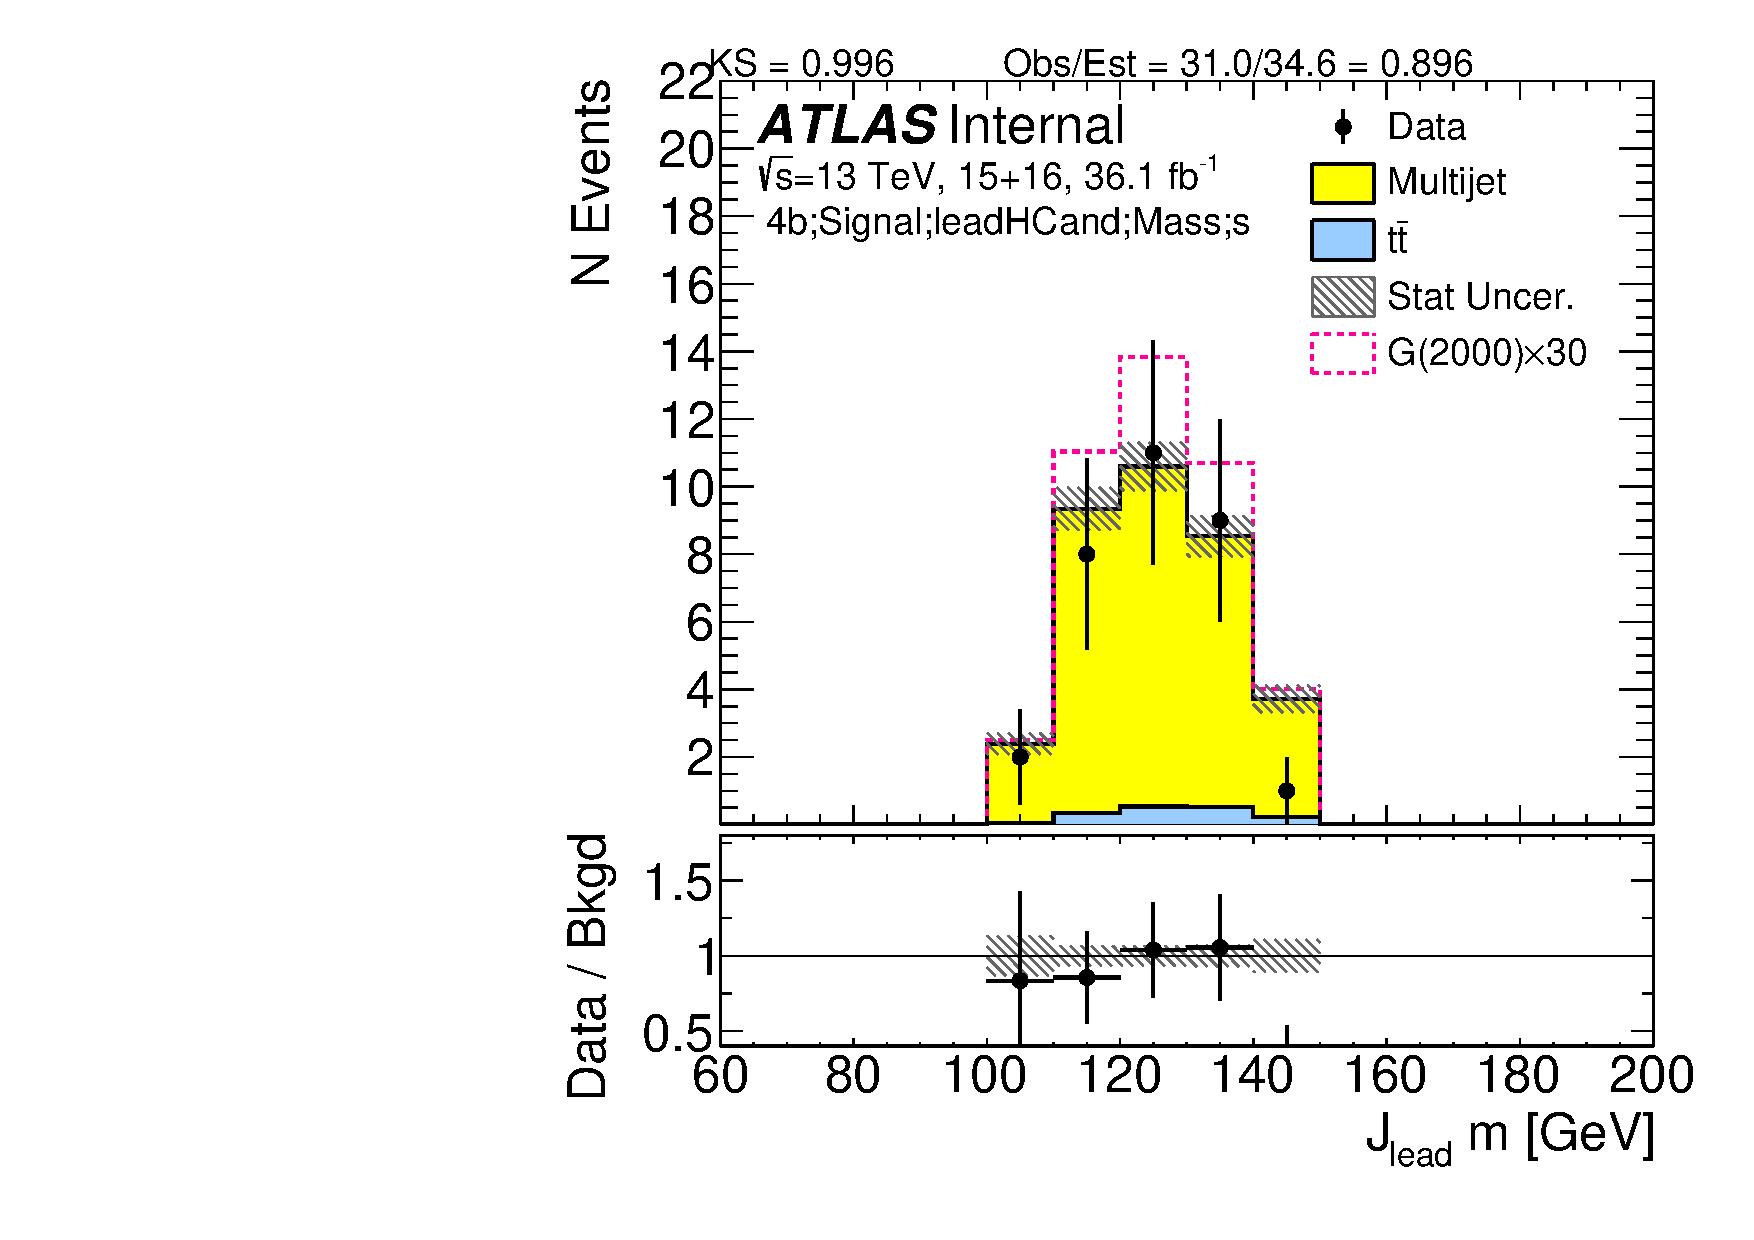
\includegraphics[width=0.31\textwidth,angle=-90]{figures/boosted/Signal/b77_FourTag_Signal_leadHCand_Mass_s.pdf}\\
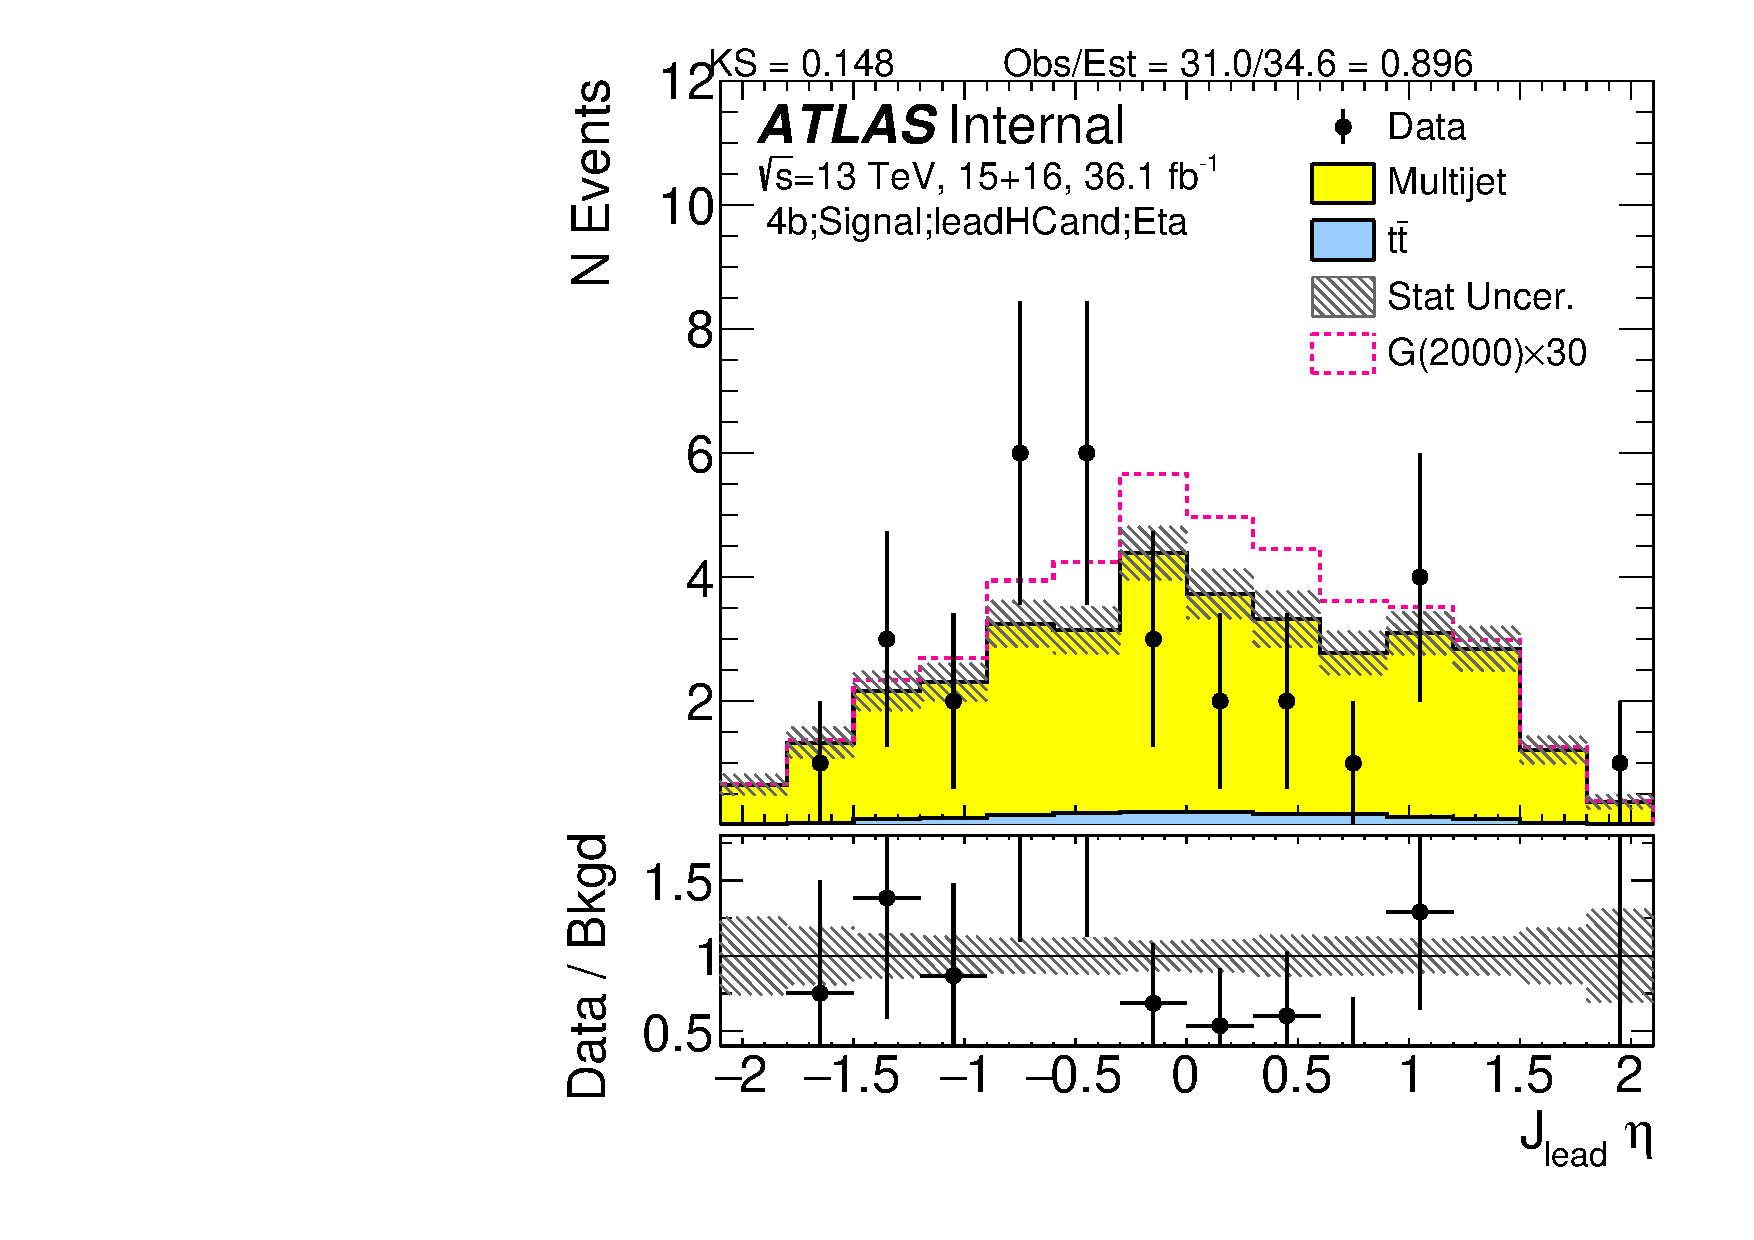
\includegraphics[width=0.31\textwidth,angle=-90]{figures/boosted/Signal/b77_FourTag_Signal_leadHCand_Eta.pdf}
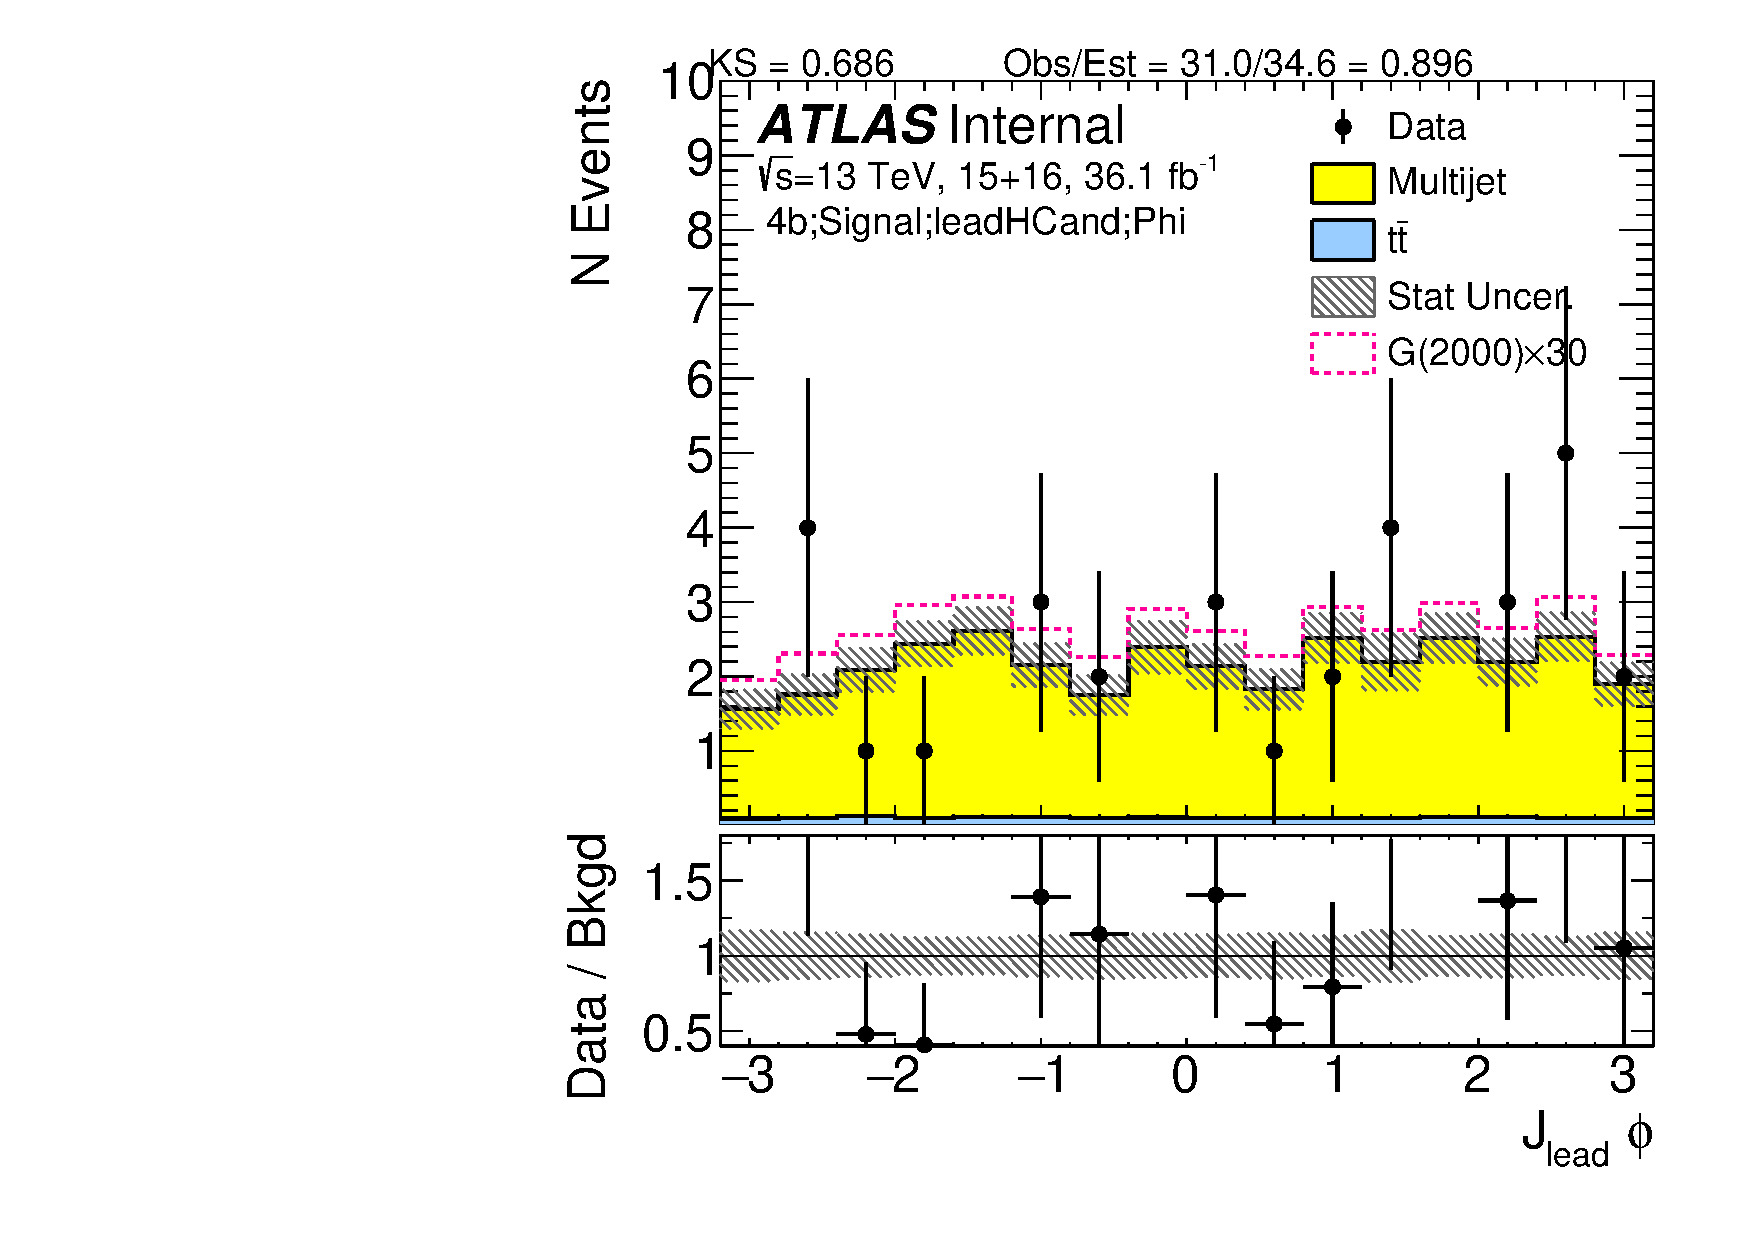
\includegraphics[width=0.31\textwidth,angle=-90]{figures/boosted/Signal/b77_FourTag_Signal_leadHCand_Phi.pdf}
  \caption{Kinematics (\pt~, mass, $\eta$, $\phi$) of the lead large-\R jet in data and prediction in the signal region after requiring 4 $b$-tags. }
  \label{fig:boosted-4b-signal-ak10-lead}
\end{center}
\end{figure*}

\begin{figure*}[htbp!]
\begin{center}
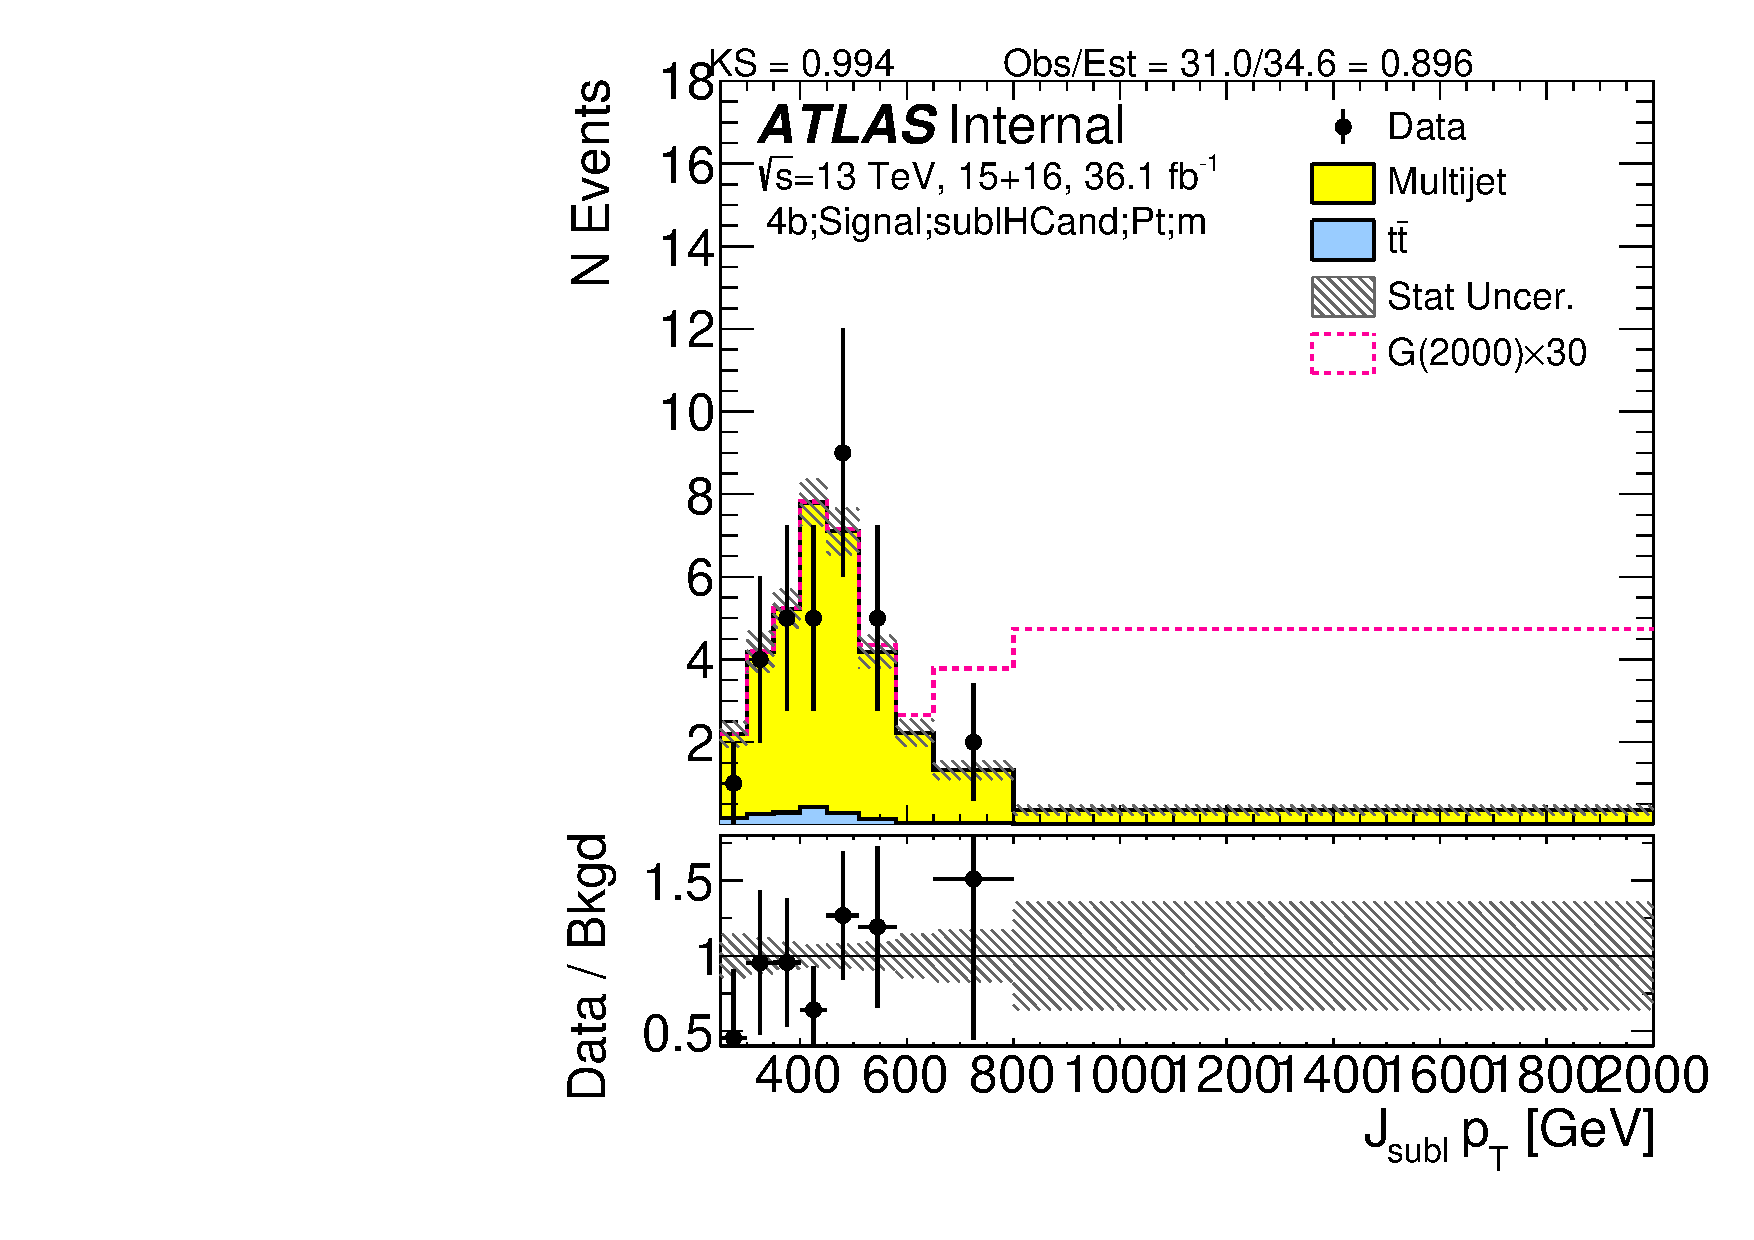
\includegraphics[width=0.31\textwidth,angle=-90]{figures/boosted/Signal/b77_FourTag_Signal_sublHCand_Pt_m.pdf}
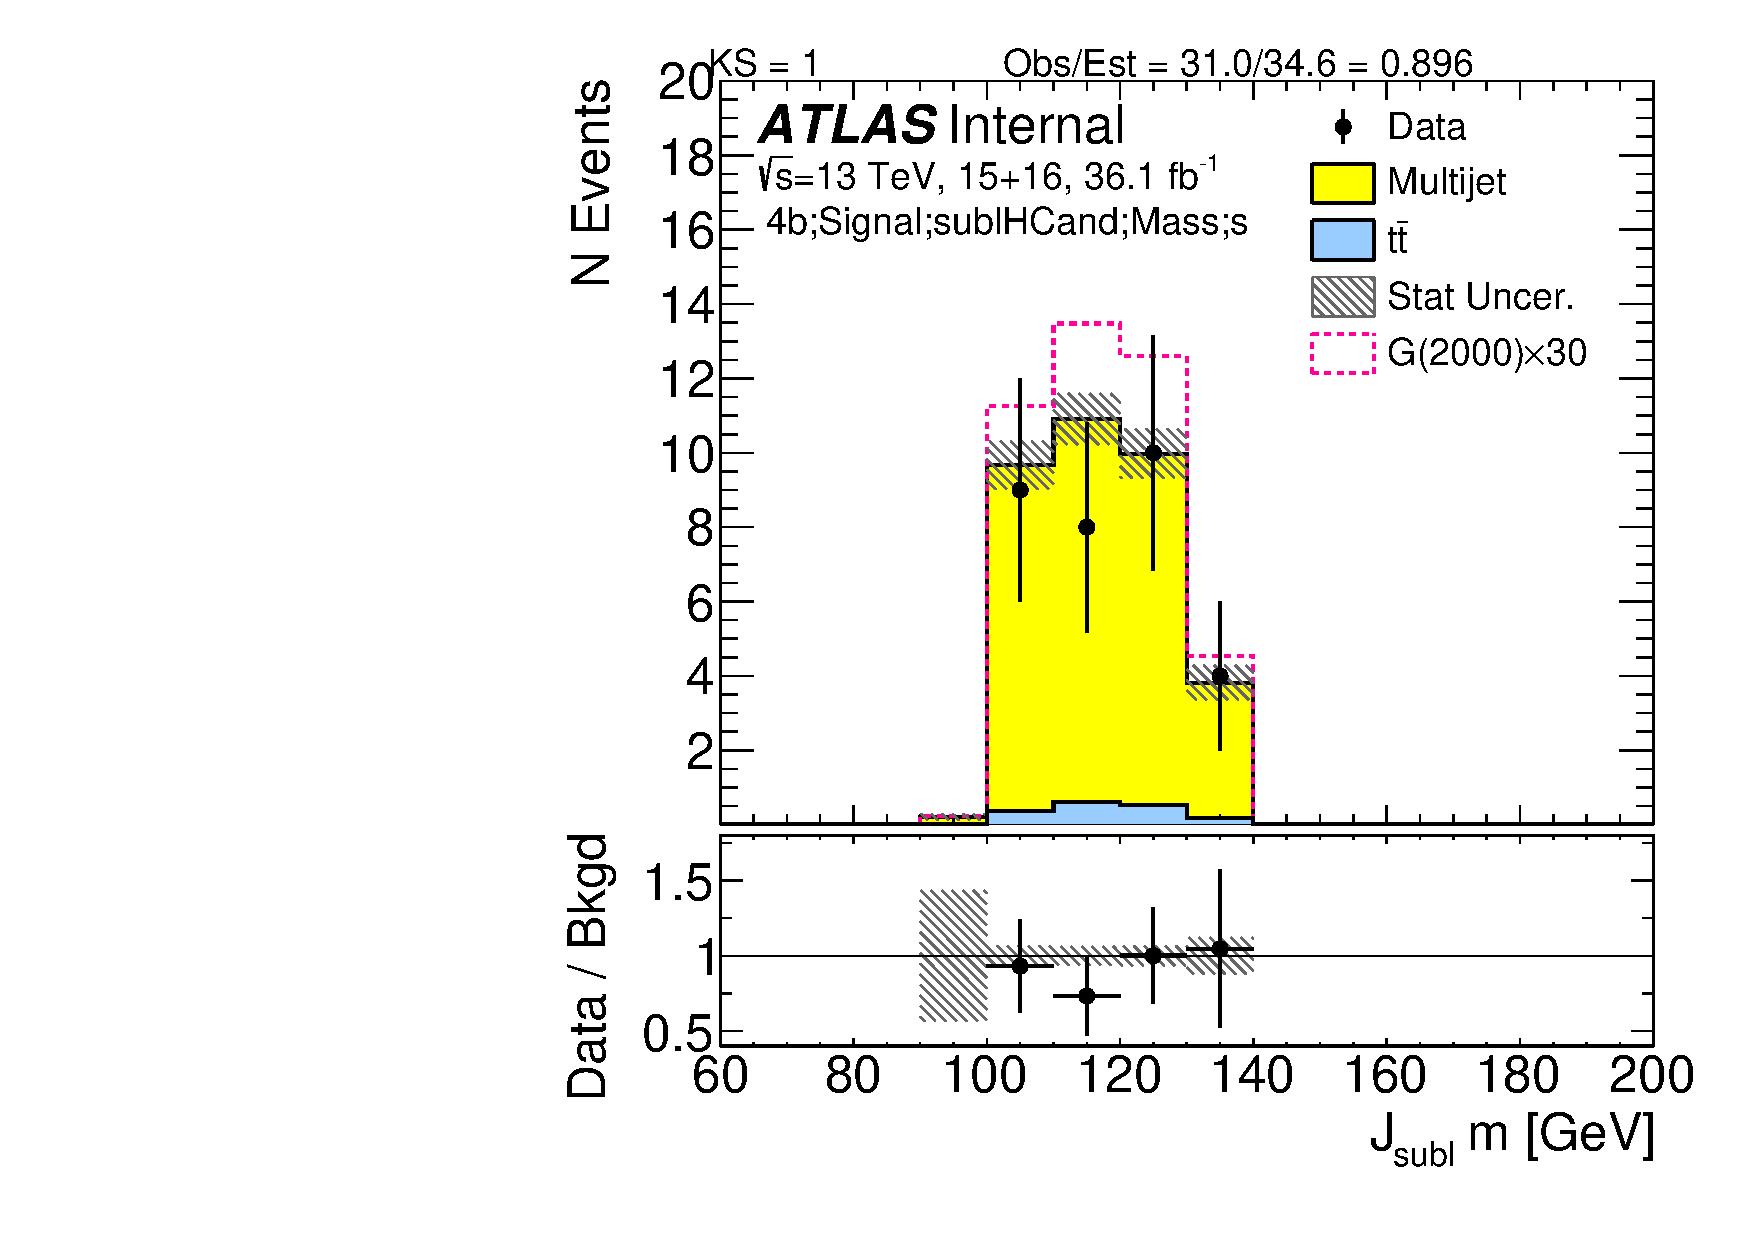
\includegraphics[width=0.31\textwidth,angle=-90]{figures/boosted/Signal/b77_FourTag_Signal_sublHCand_Mass_s.pdf}\\
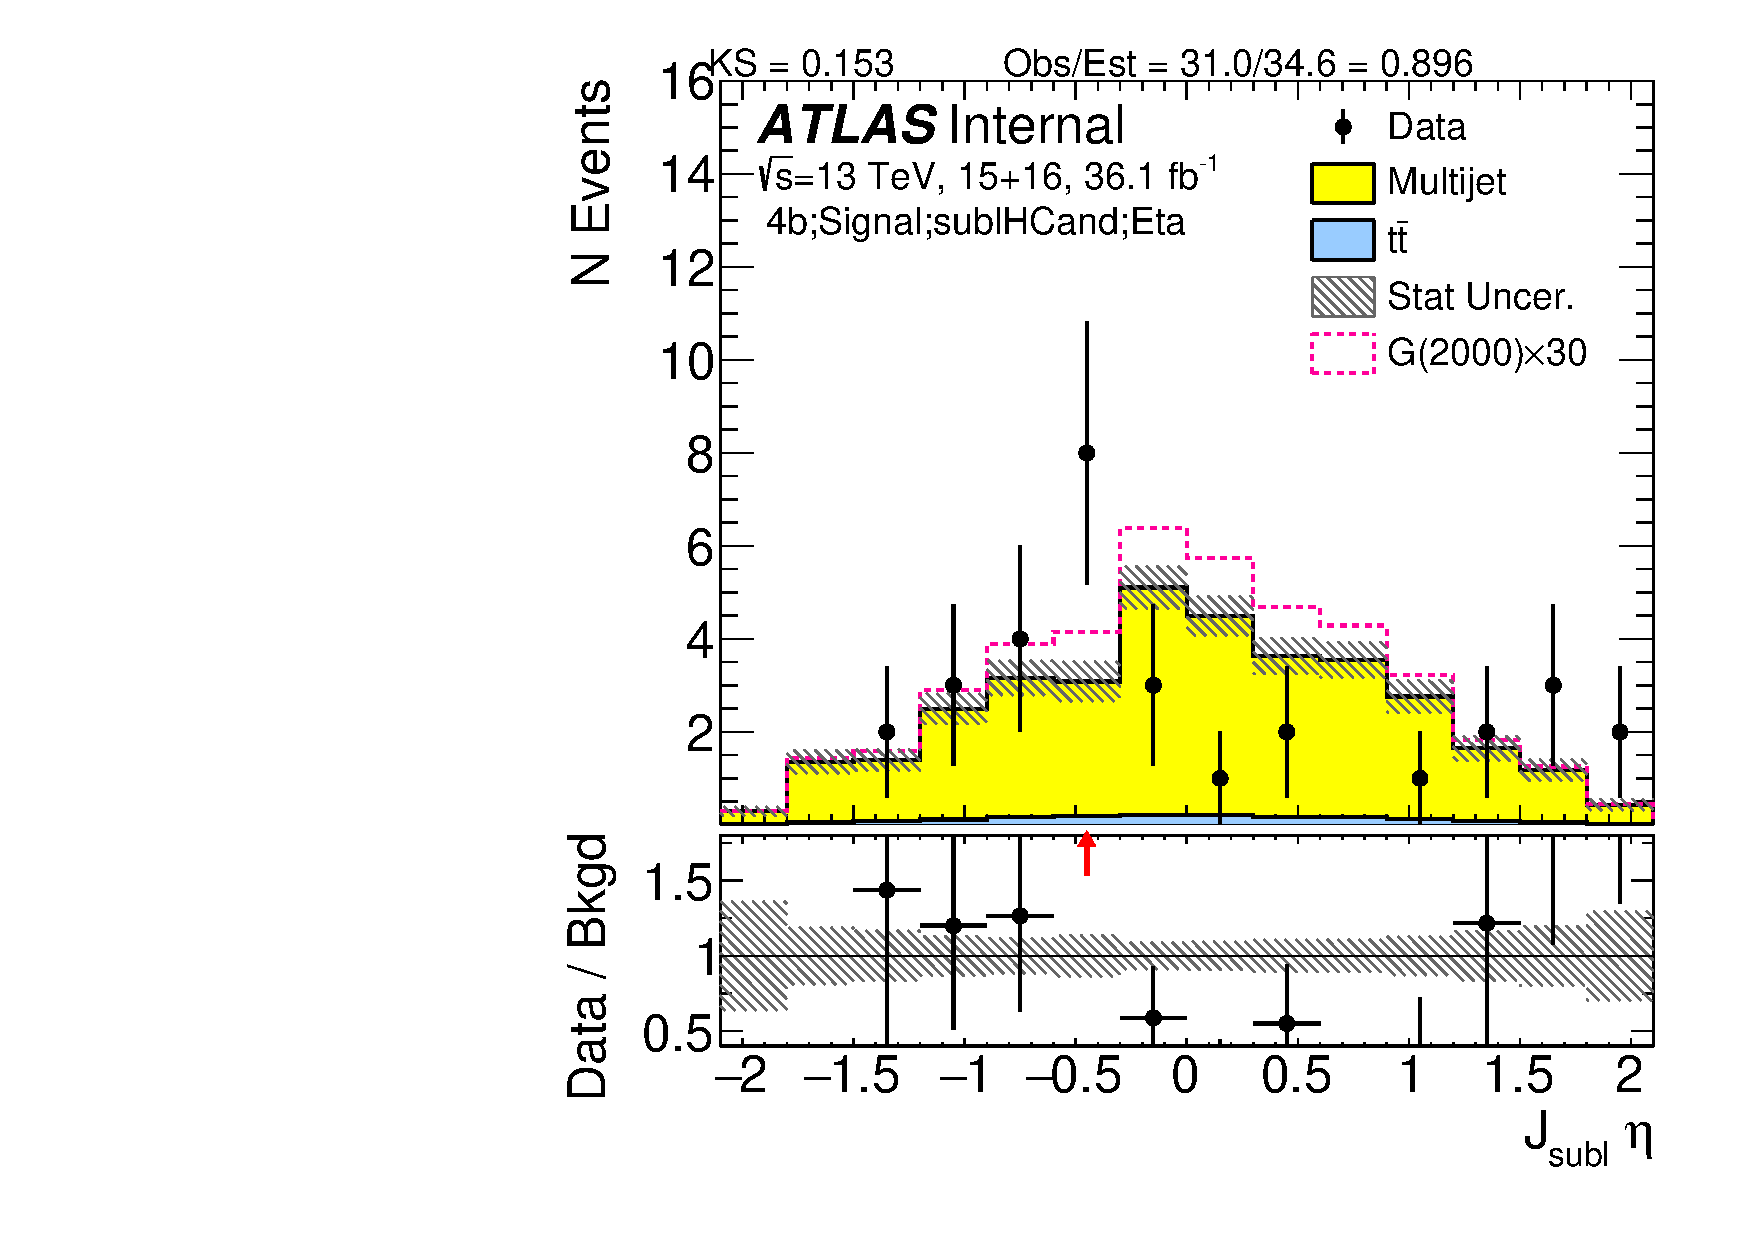
\includegraphics[width=0.31\textwidth,angle=-90]{figures/boosted/Signal/b77_FourTag_Signal_sublHCand_Eta.pdf}
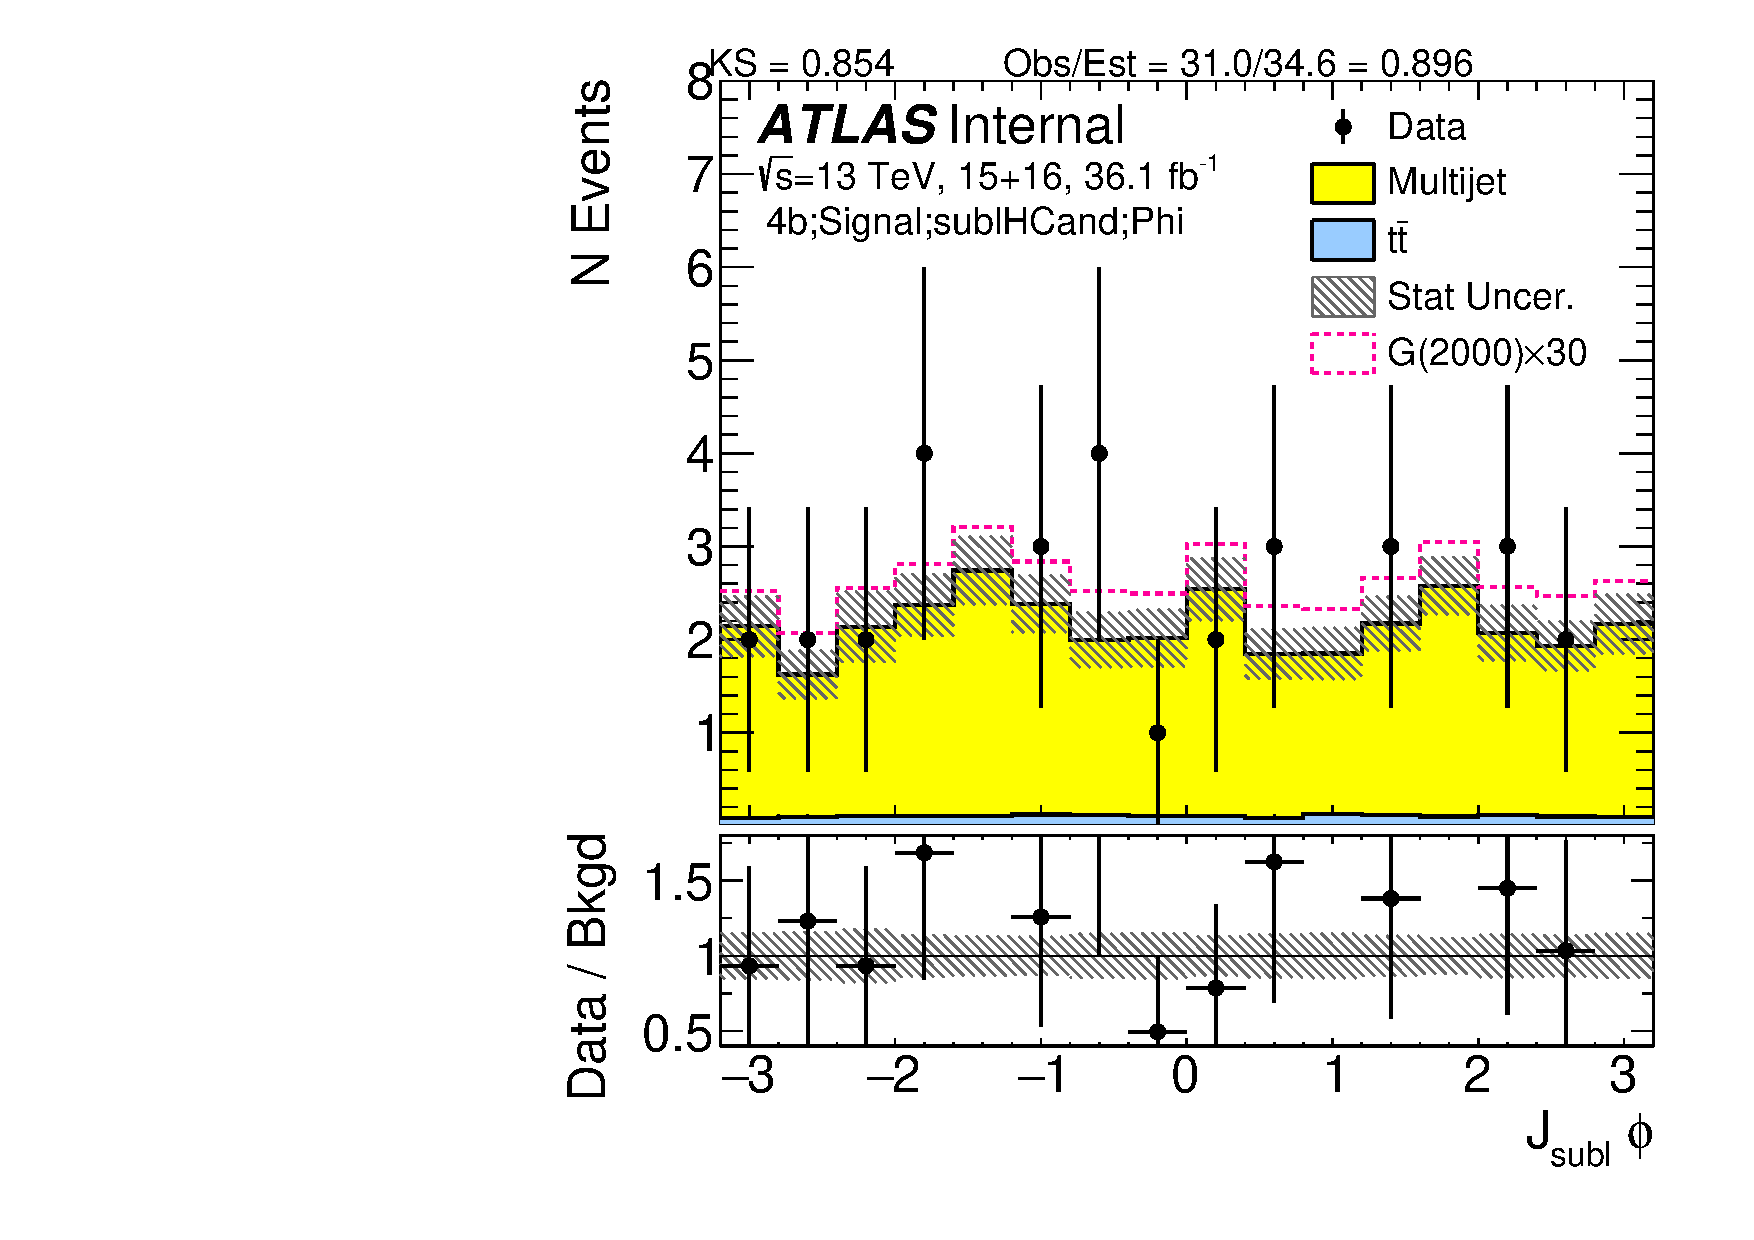
\includegraphics[width=0.31\textwidth,angle=-90]{figures/boosted/Signal/b77_FourTag_Signal_sublHCand_Phi.pdf}
  \caption{Kinematics (\pt~, mass, $\eta$, $\phi$) of the subleading large-\R jet in data and prediction in the signal region after requiring 4 $b$-tags. }
  \label{fig:boosted-4b-signal-ak10-subl}
\end{center}
\end{figure*}

\begin{figure*}[htbp!]
\begin{center}
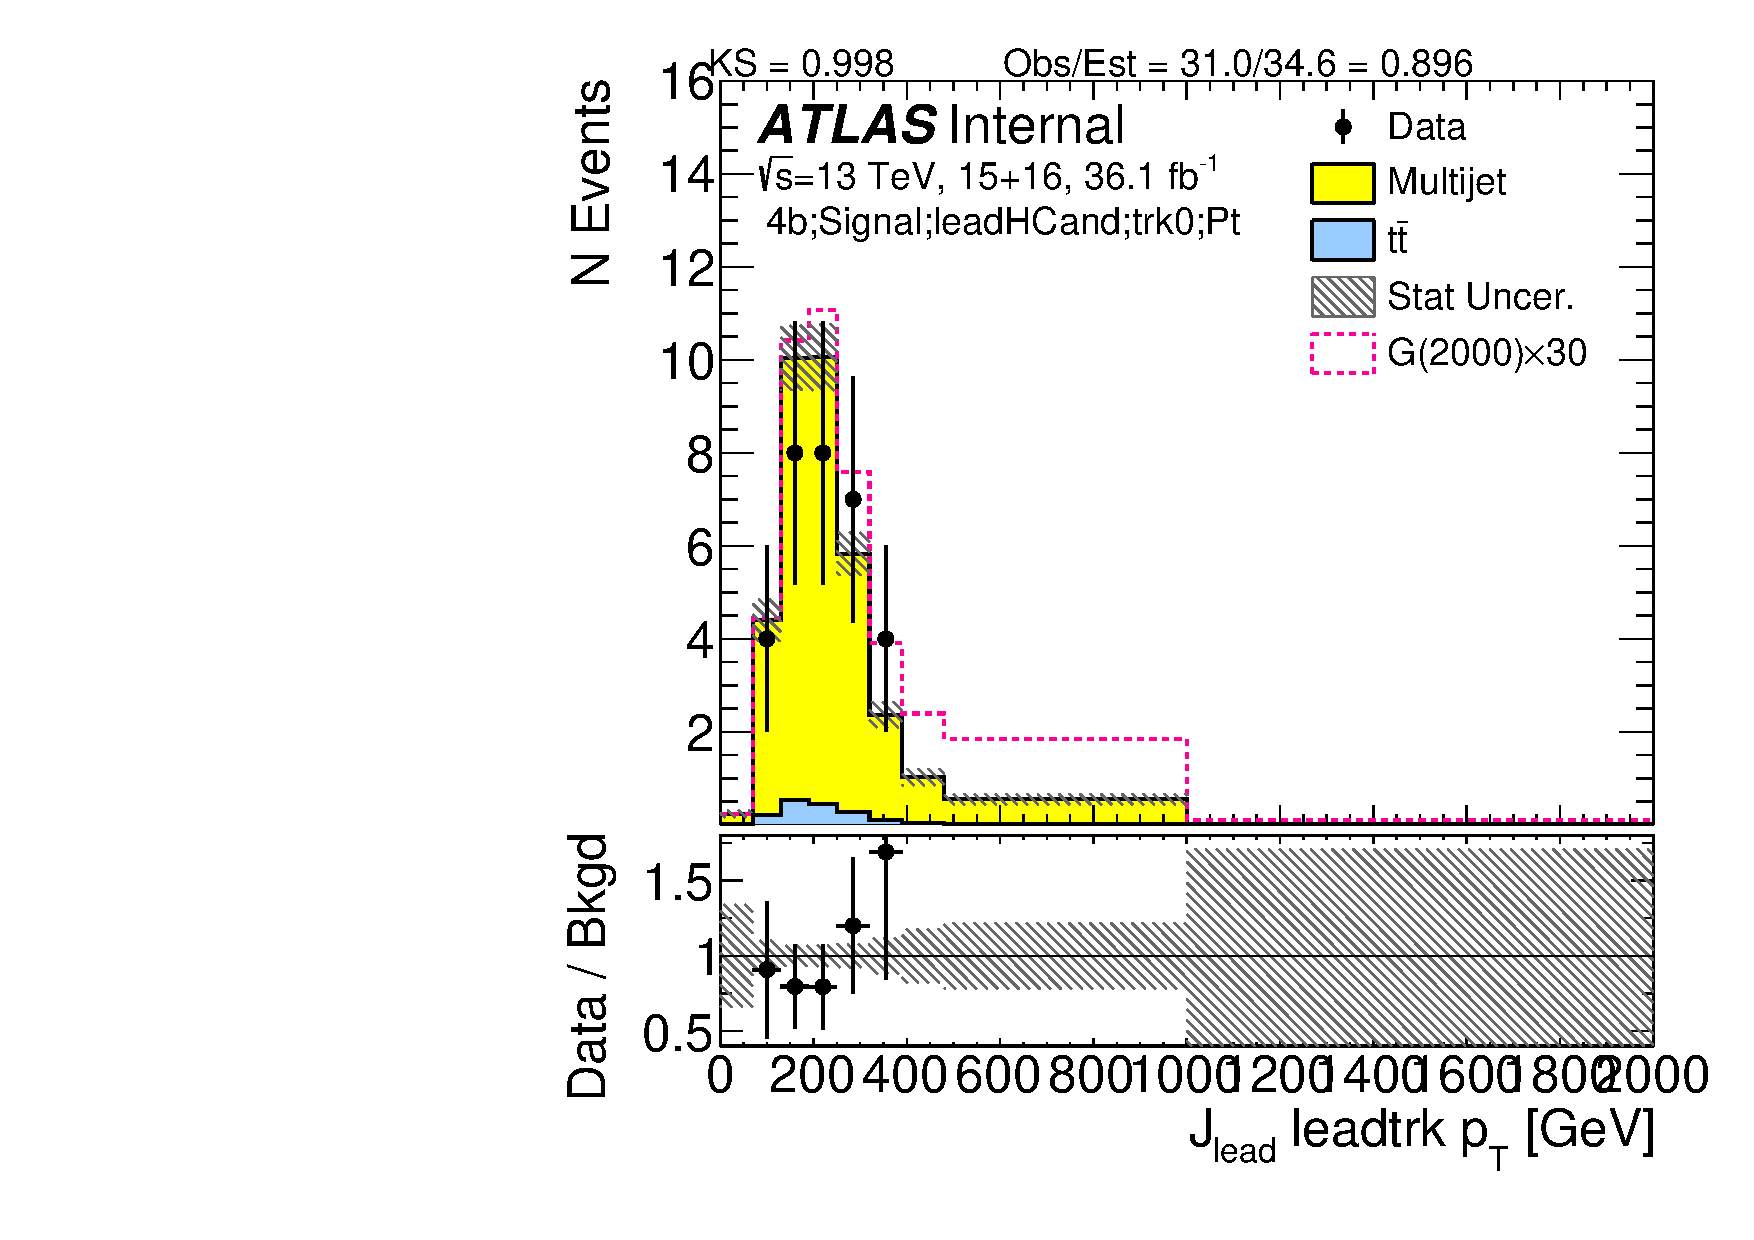
\includegraphics[width=0.31\textwidth,angle=-90]{figures/boosted/Signal/b77_FourTag_Signal_leadHCand_trk0_Pt.pdf}
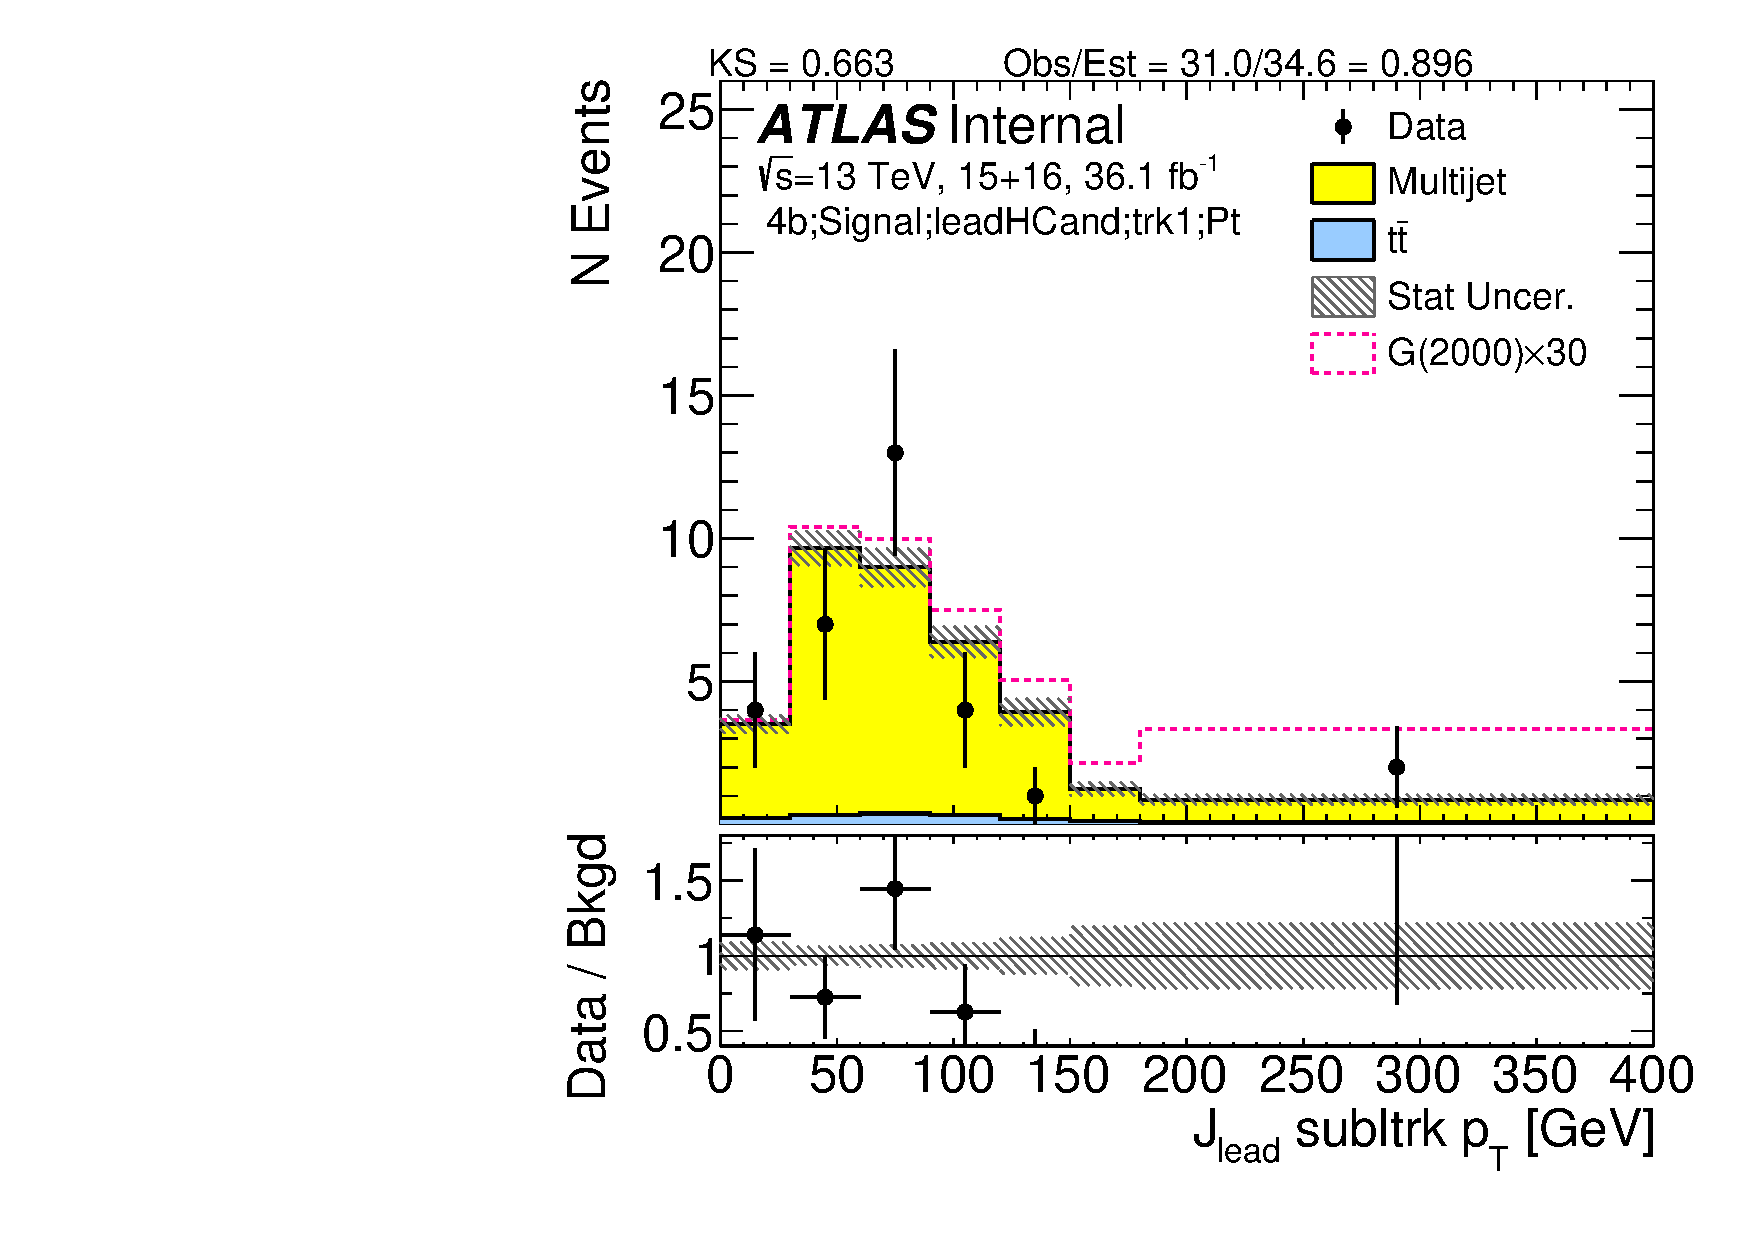
\includegraphics[width=0.31\textwidth,angle=-90]{figures/boosted/Signal/b77_FourTag_Signal_leadHCand_trk1_Pt.pdf}\\
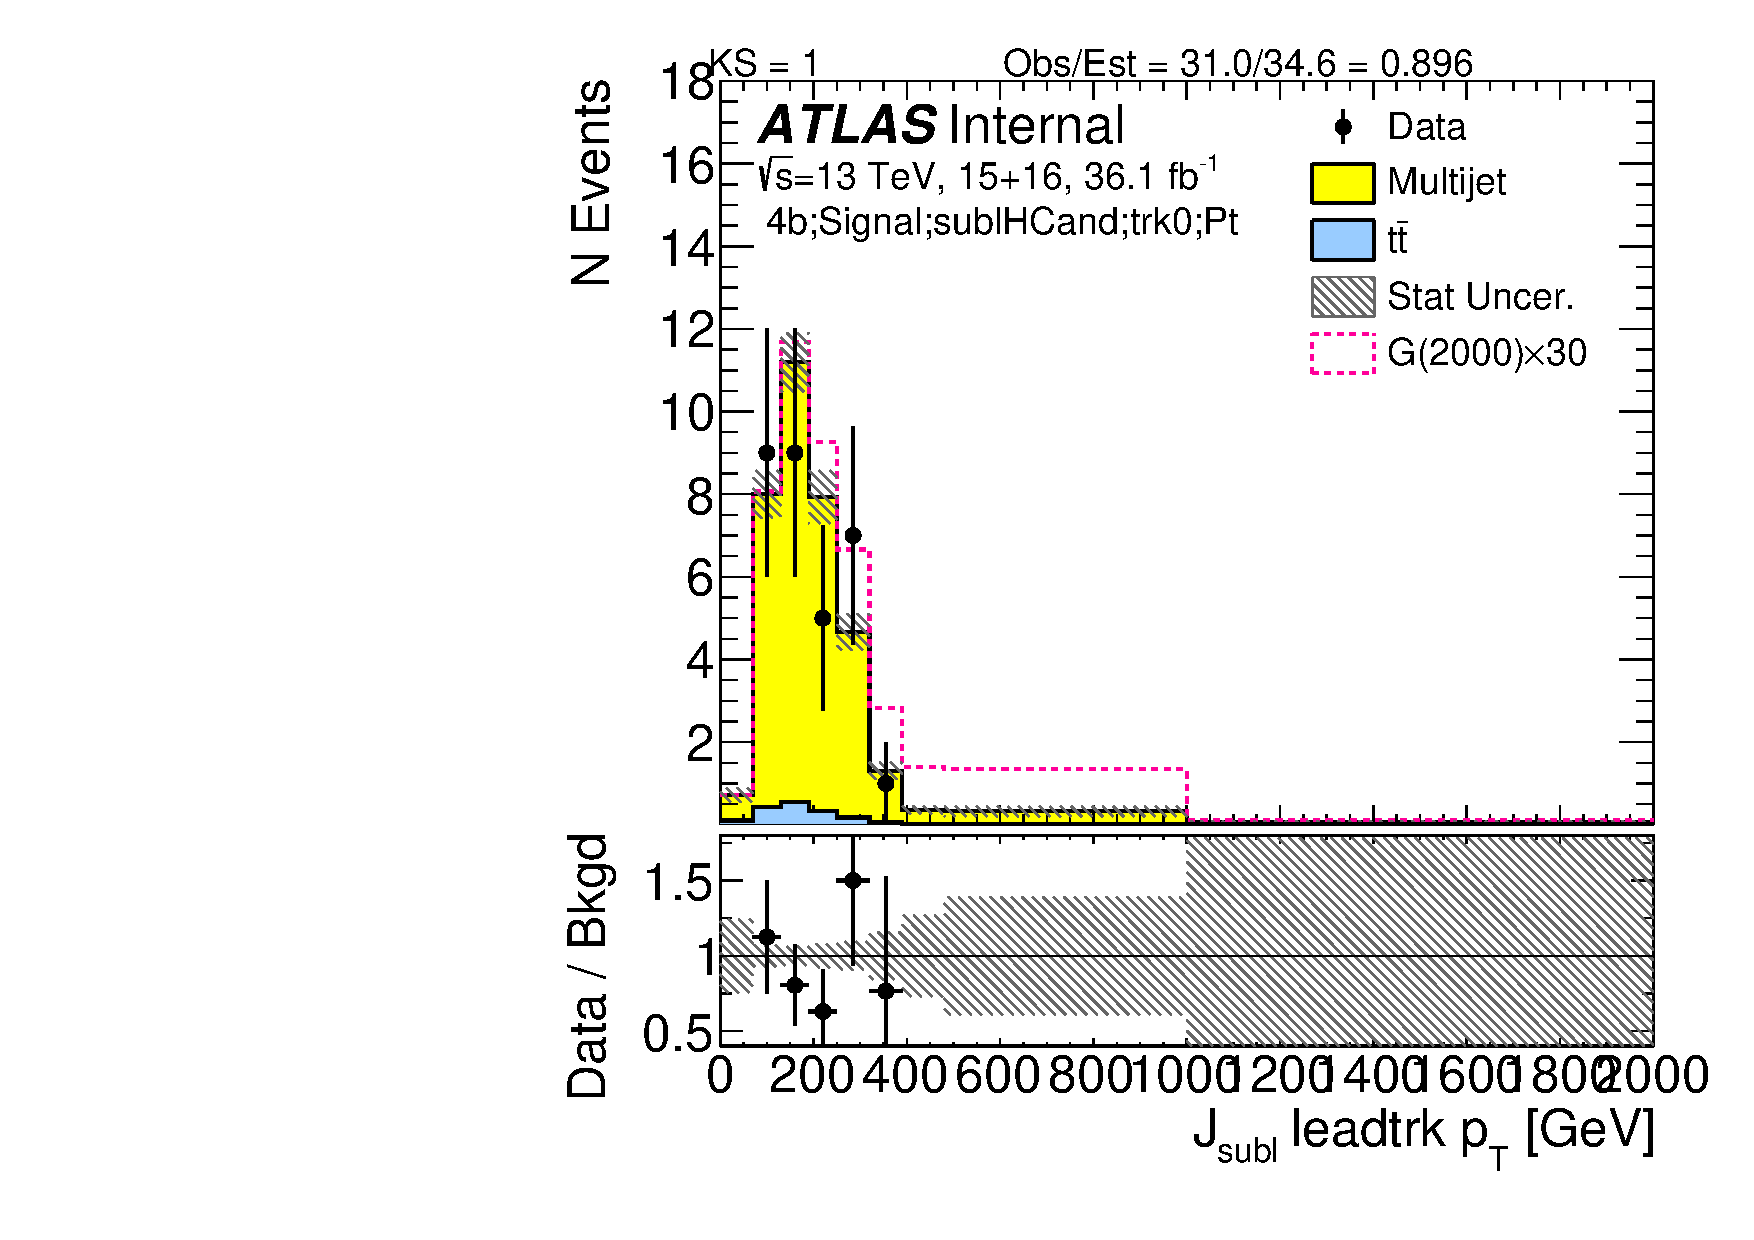
\includegraphics[width=0.31\textwidth,angle=-90]{figures/boosted/Signal/b77_FourTag_Signal_sublHCand_trk0_Pt.pdf}
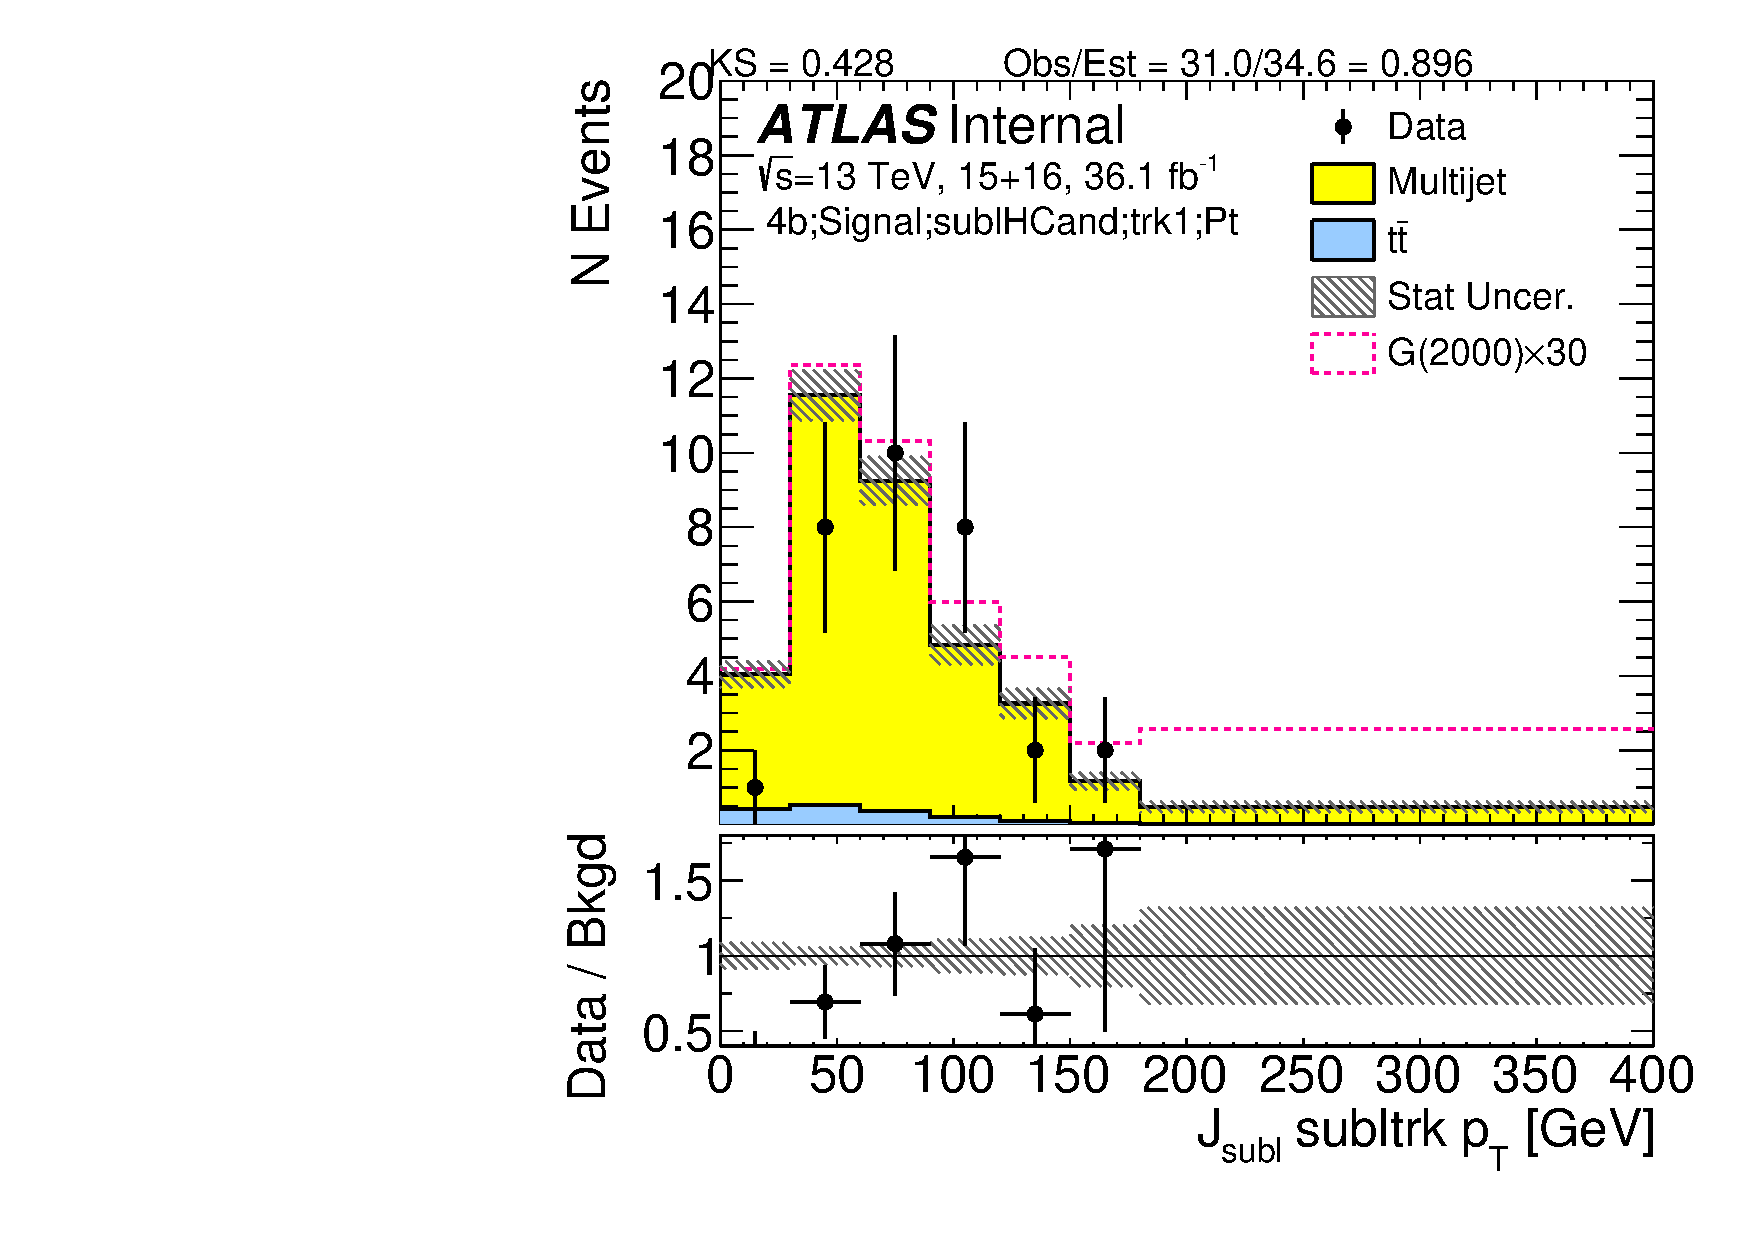
\includegraphics[width=0.31\textwidth,angle=-90]{figures/boosted/Signal/b77_FourTag_Signal_sublHCand_trk1_Pt.pdf}\\
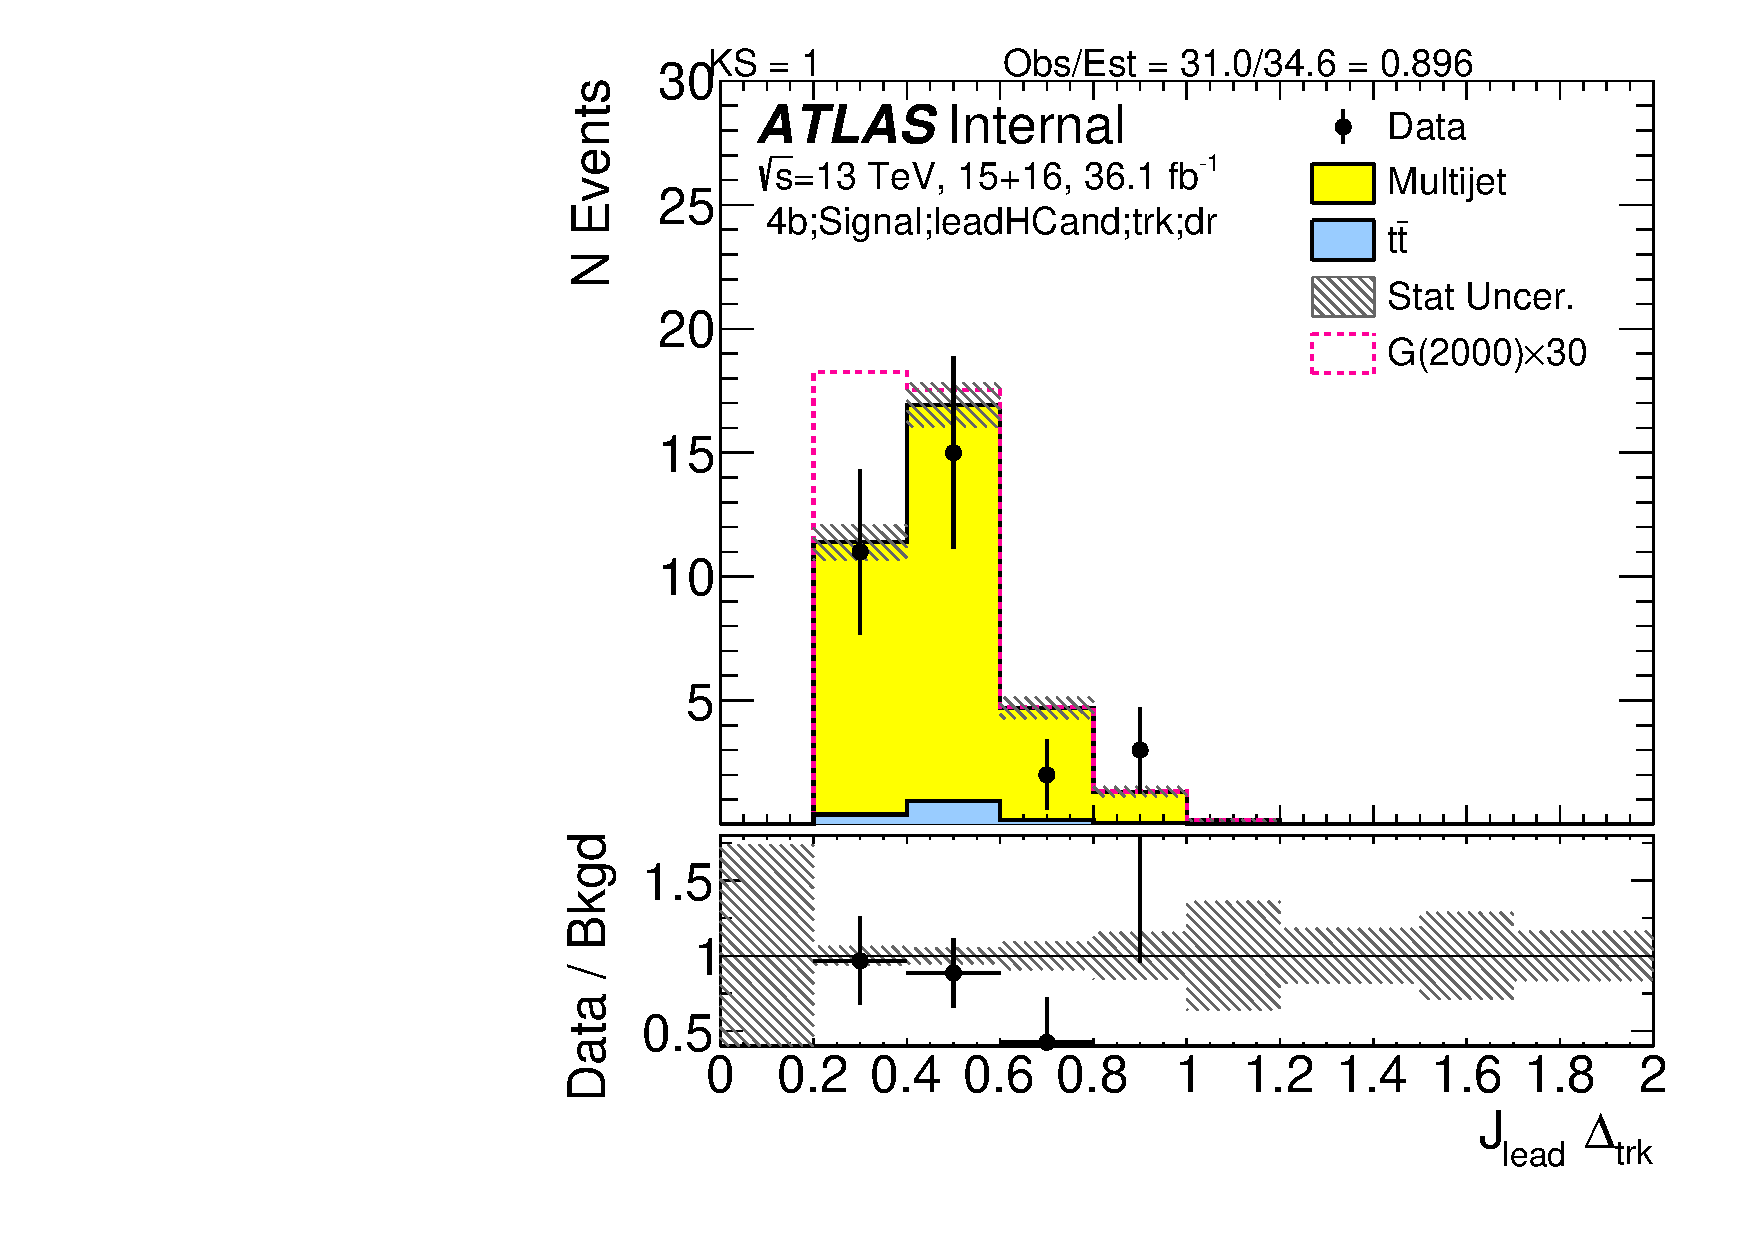
\includegraphics[width=0.31\textwidth,angle=-90]{figures/boosted/Signal/b77_FourTag_Signal_leadHCand_trk_dr.pdf}
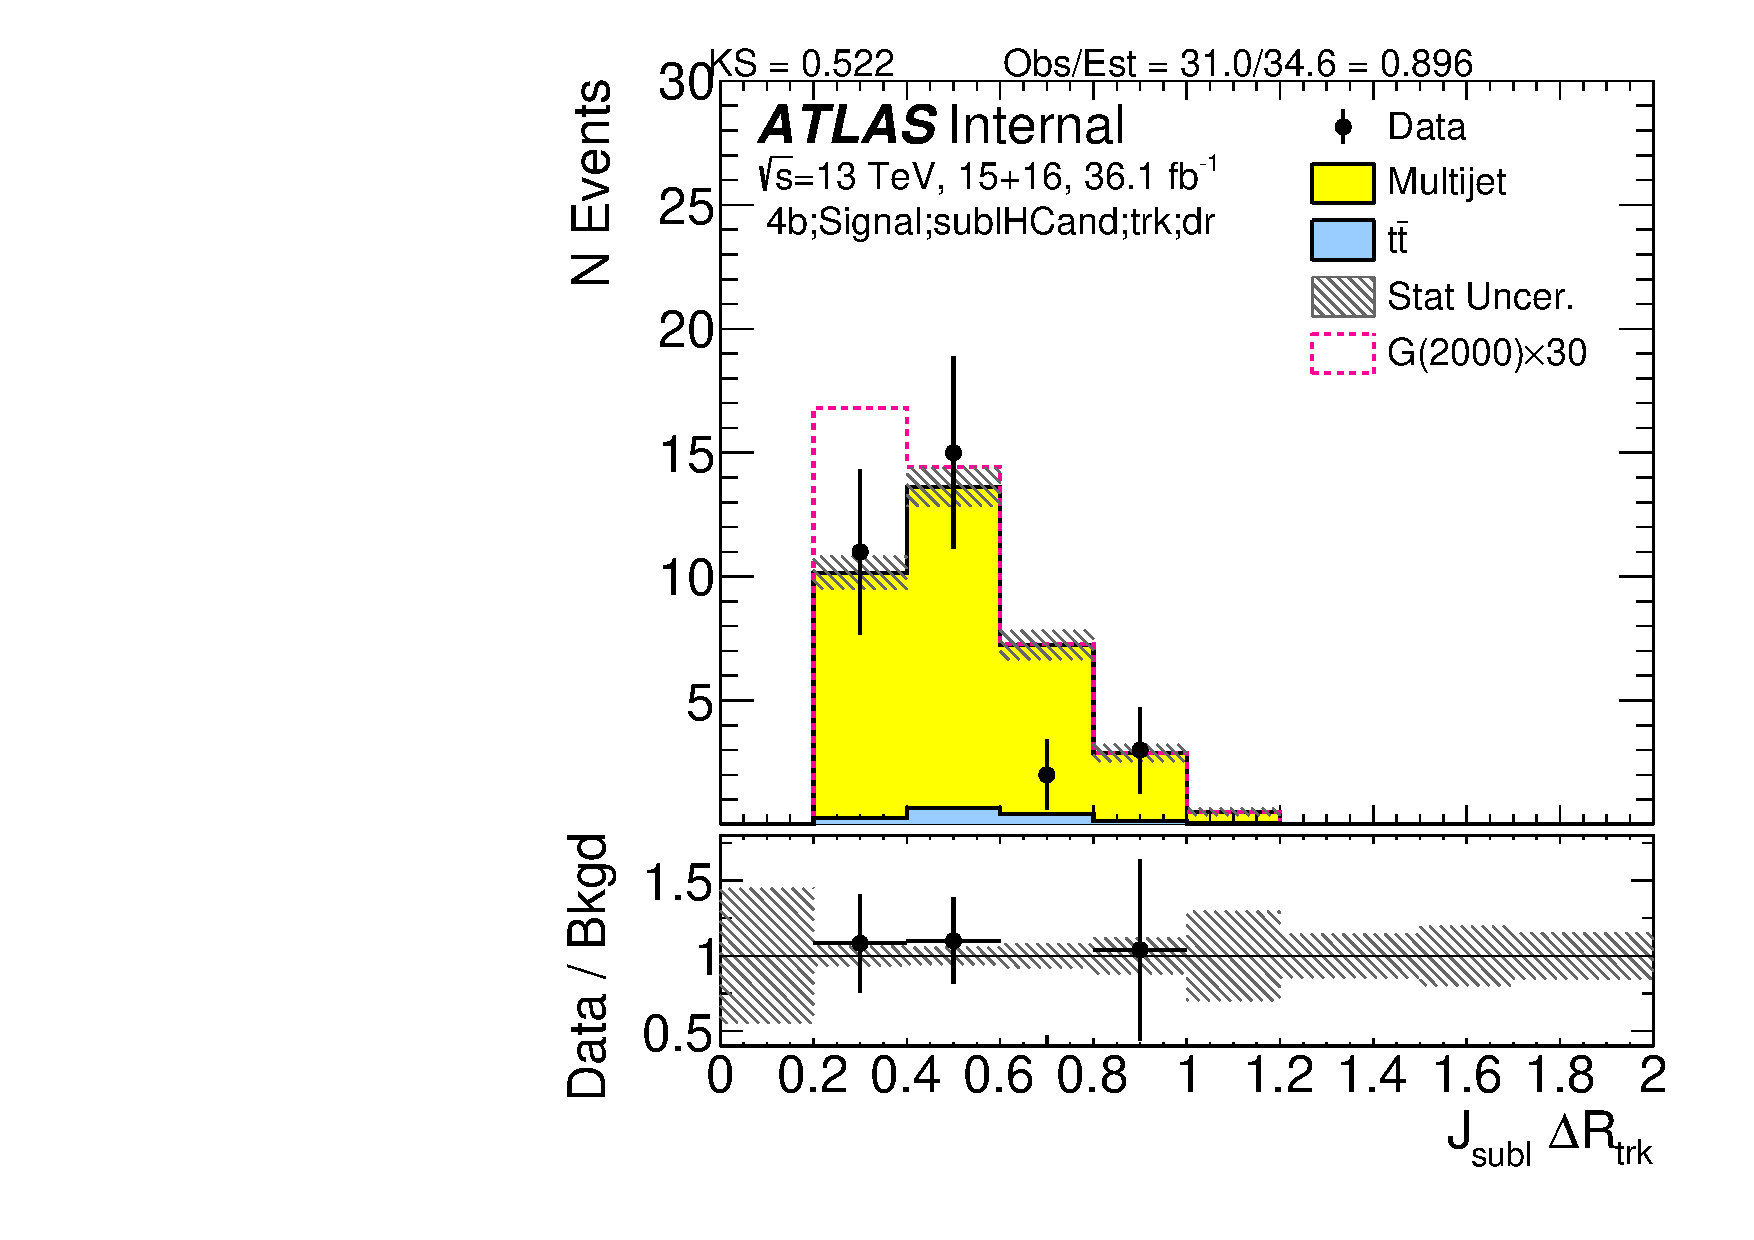
\includegraphics[width=0.31\textwidth,angle=-90]{figures/boosted/Signal/b77_FourTag_Signal_sublHCand_trk_dr.pdf}
  \caption{First two rows show the \pt~ of the lead (left) and sub-lead (right) small-$R$ track jets associated to the lead (first-row) and sub-lead (second-row) large-\R jet in data and prediction in the signal region after requiring 4 $b$-tags. Third row shows the $\Delta R$ between two leading small-$R$ track-jets associated to the leading (left) and sub-leading (right) large-\R jet.  }
  \label{fig:boosted-4b-signal-ak2}
\end{center}
\end{figure*}


\begin{figure*}[htbp!]
\begin{center}
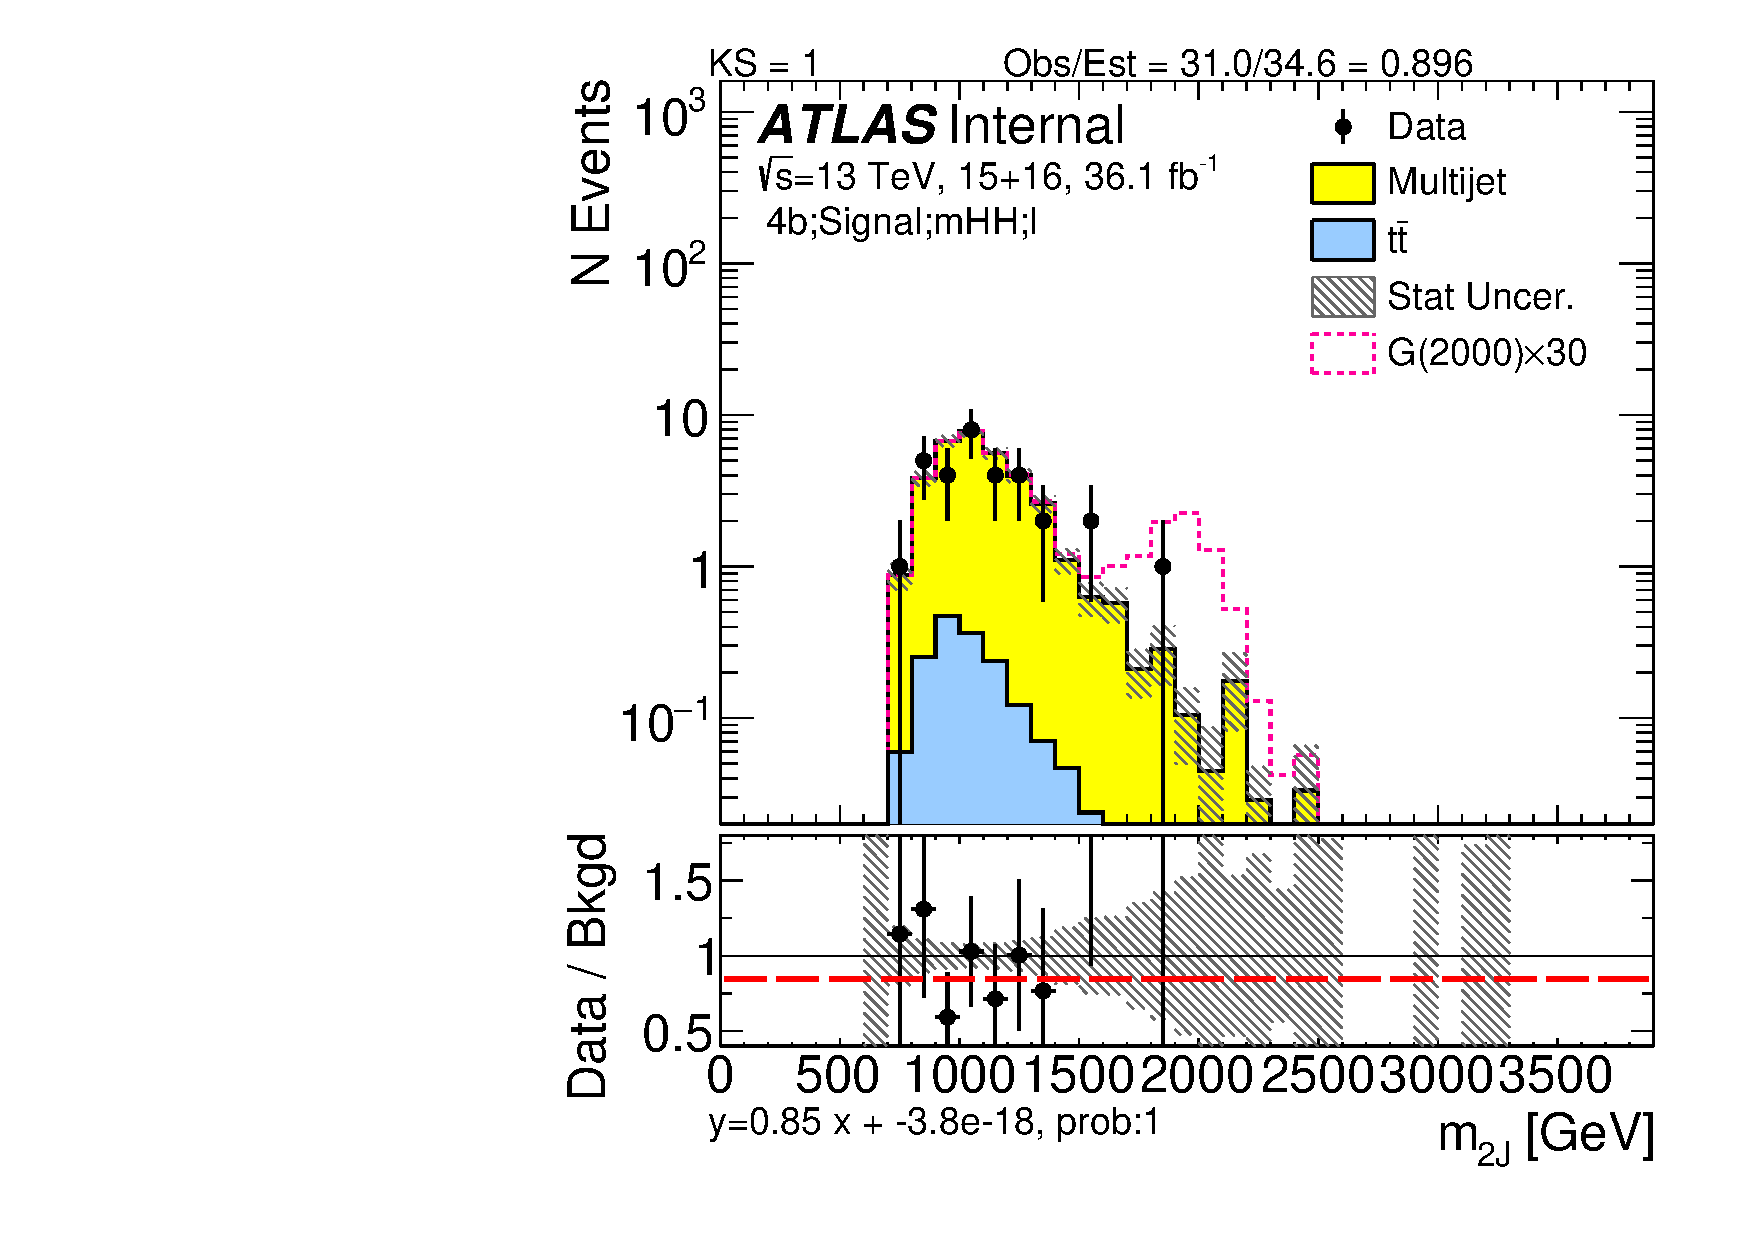
\includegraphics[width=0.31\textwidth,angle=-90]{figures/boosted/Signal/b77_FourTag_Signal_mHH_l_1.pdf}
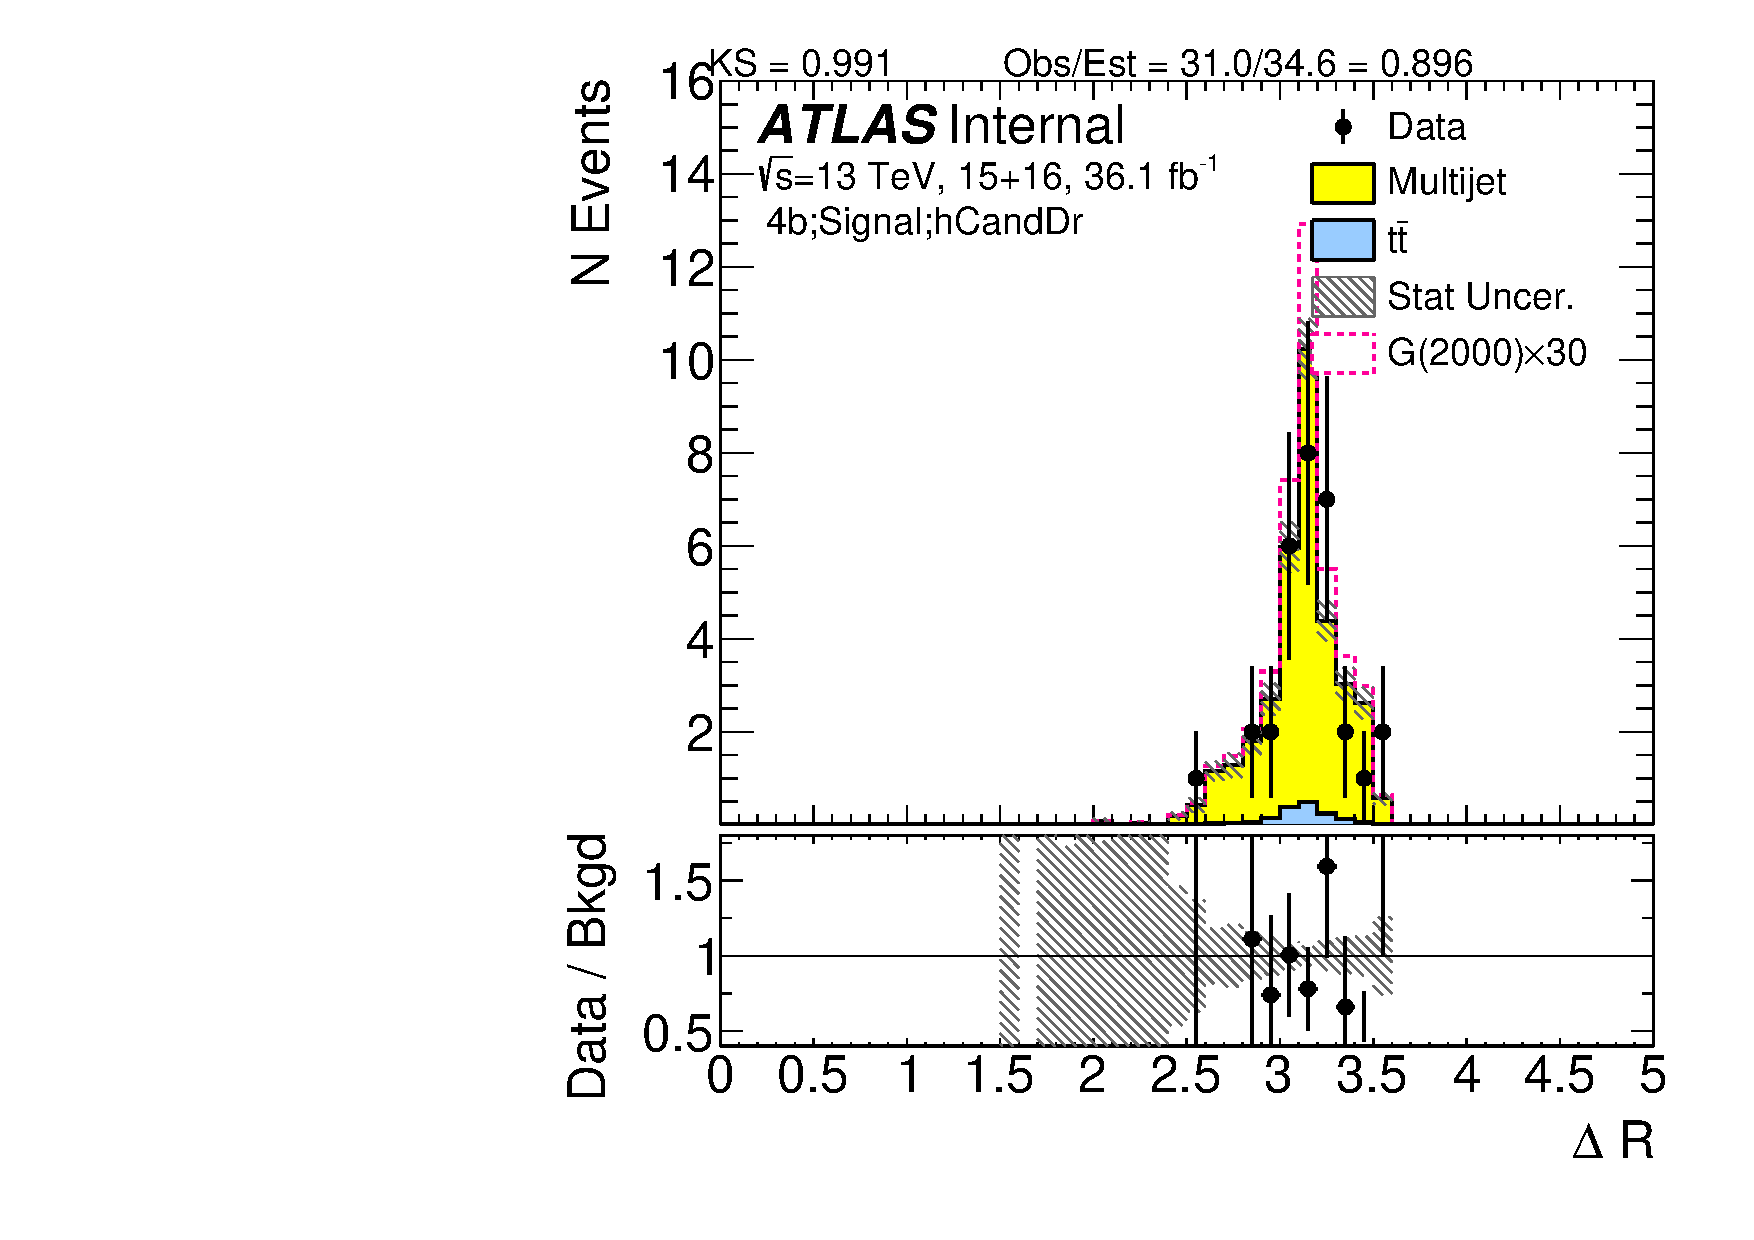
\includegraphics[width=0.31\textwidth,angle=-90]{figures/boosted/Signal/b77_FourTag_Signal_hCandDr.pdf}\\
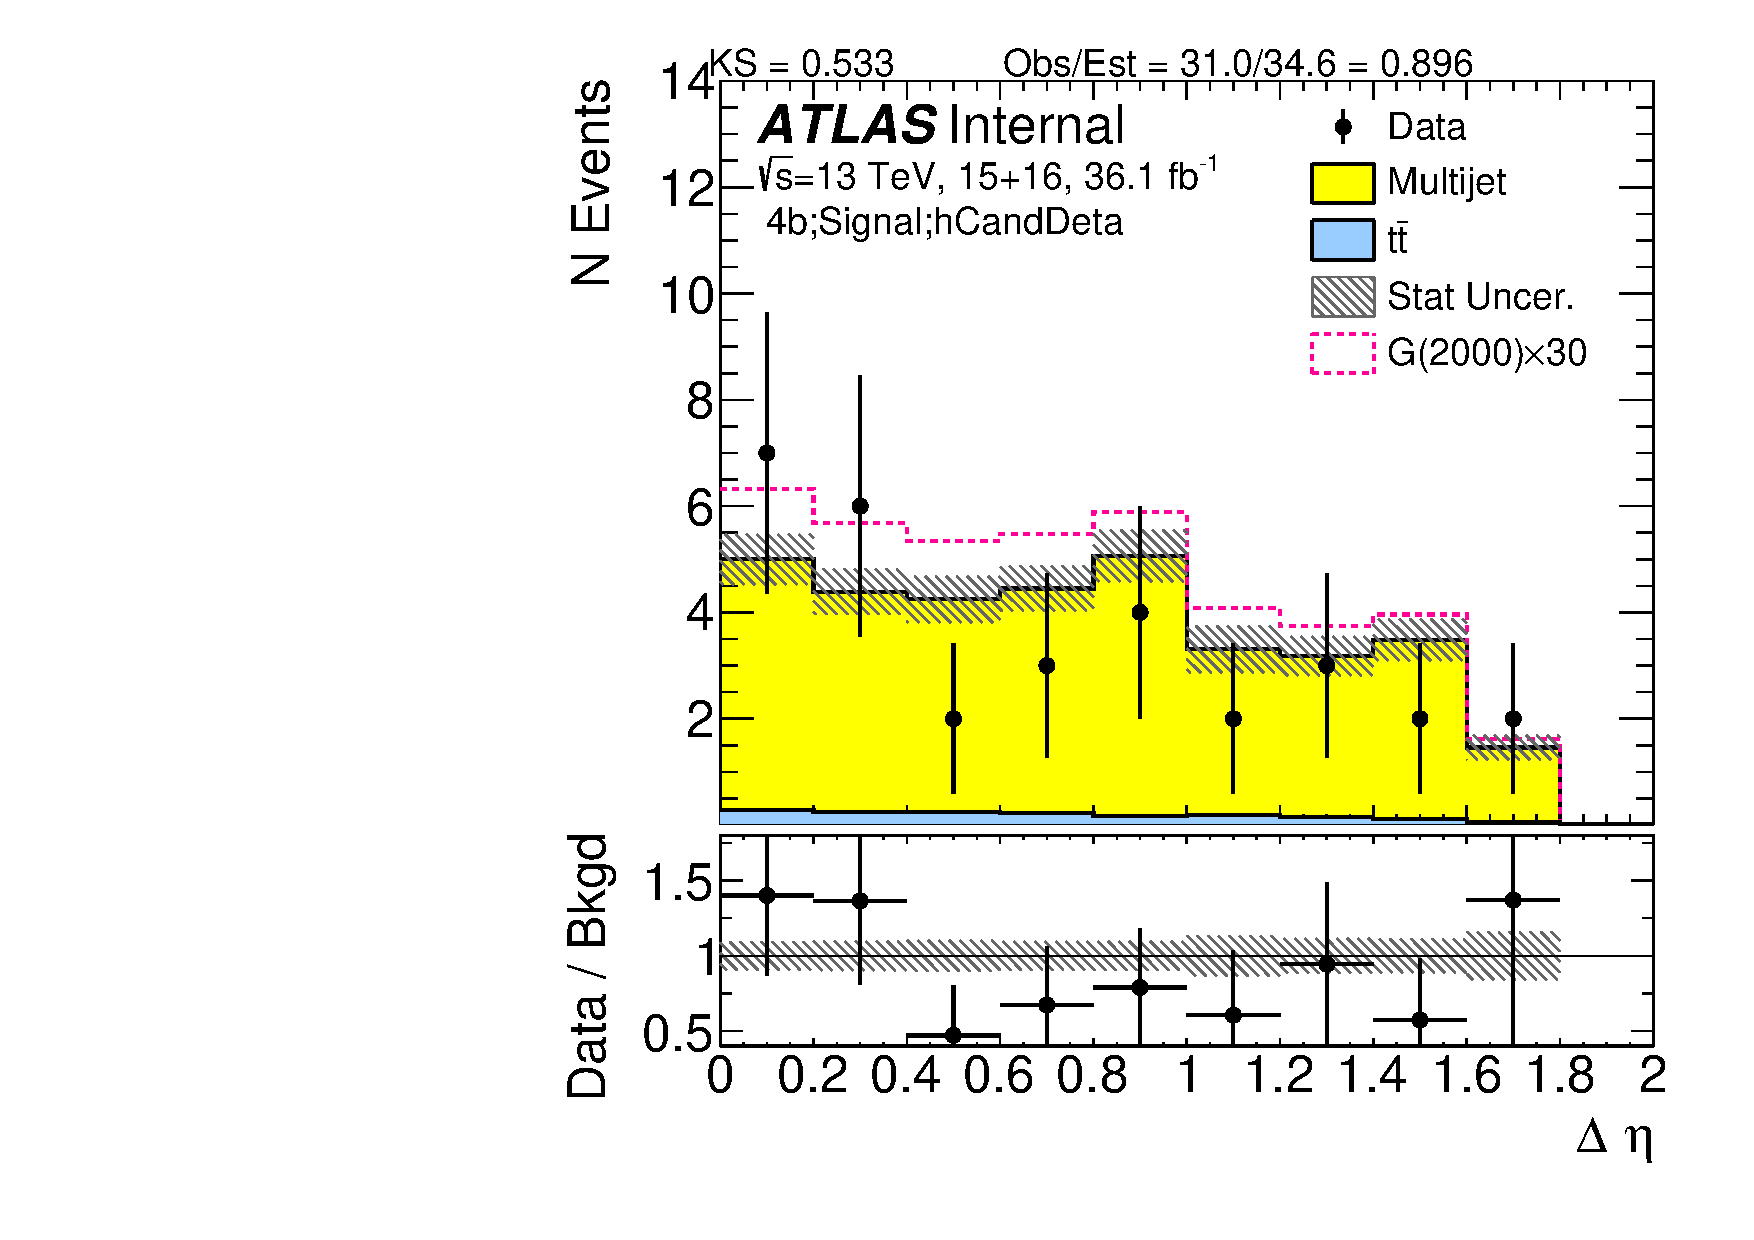
\includegraphics[width=0.31\textwidth,angle=-90]{figures/boosted/Signal/b77_FourTag_Signal_hCandDeta.pdf}
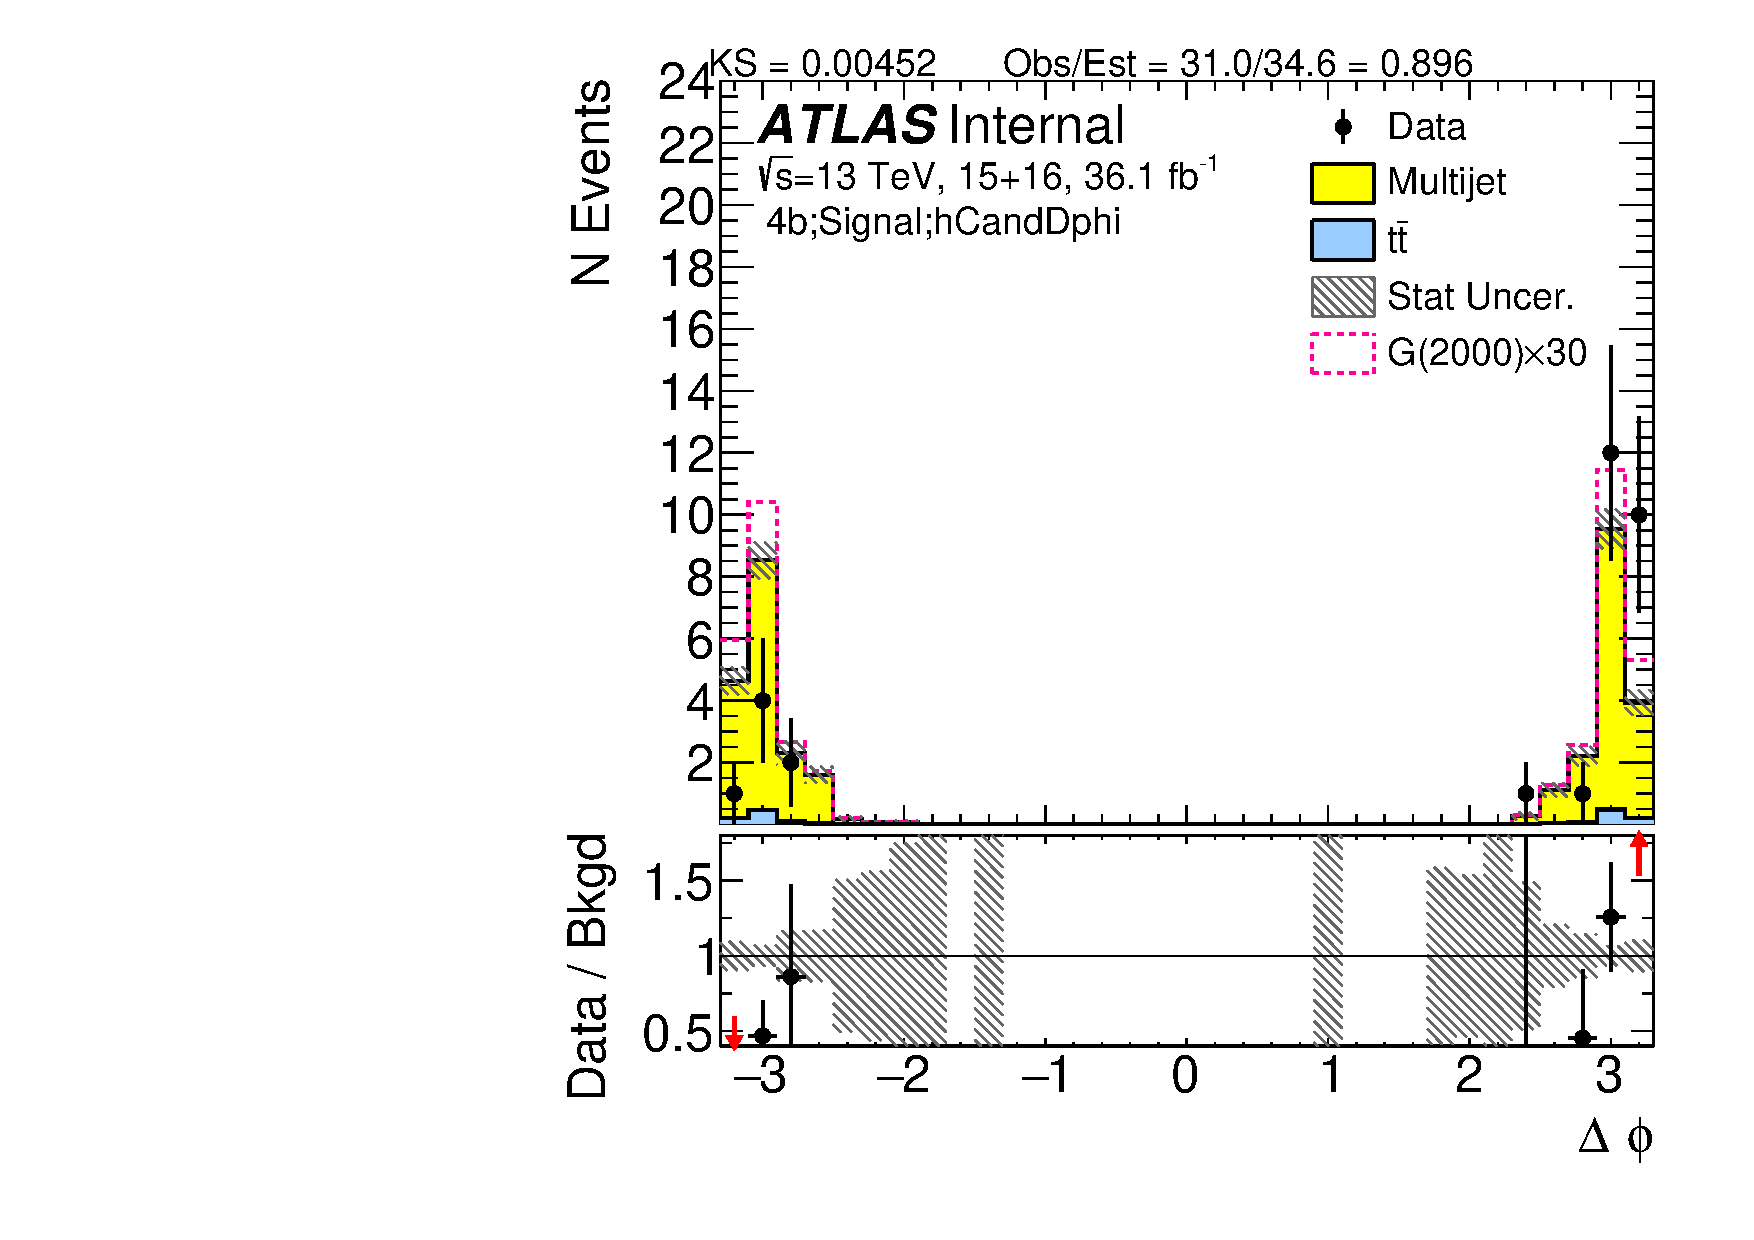
\includegraphics[width=0.31\textwidth,angle=-90]{figures/boosted/Signal/b77_FourTag_Signal_hCandDphi.pdf}
  \caption{Kinematics (invariant mass, $\Delta R$, $\Delta \eta$ and $\Delta \phi$) of two large-\R jets in data and prediction in the signal region after requiring 4 $b$-tags.  }
  \label{fig:boosted-4b-signal-ak10-system}
\end{center}
\end{figure*}

\clearpage

\begin{figure*}[htbp!]
\begin{center}
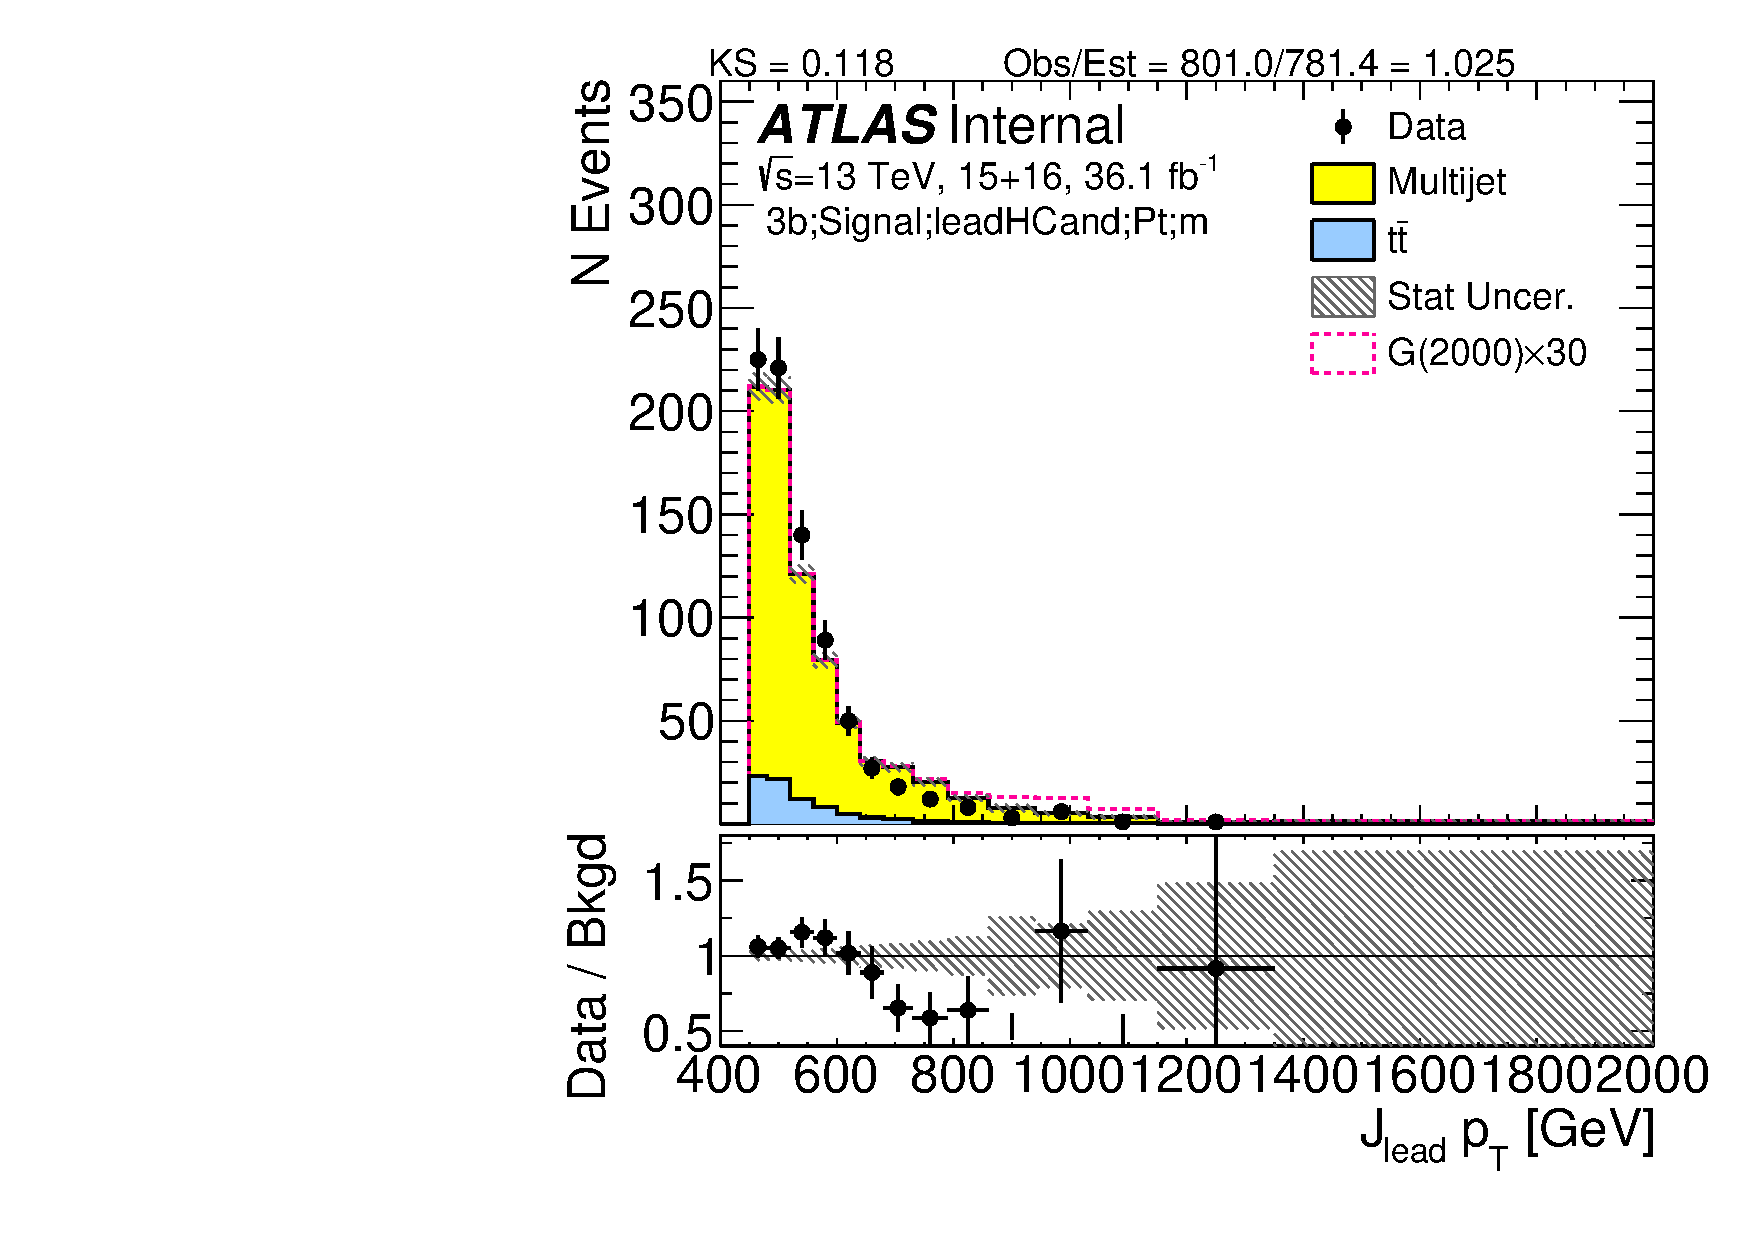
\includegraphics[width=0.31\textwidth,angle=-90]{figures/boosted/Signal/b77_ThreeTag_Signal_leadHCand_Pt_m.pdf}
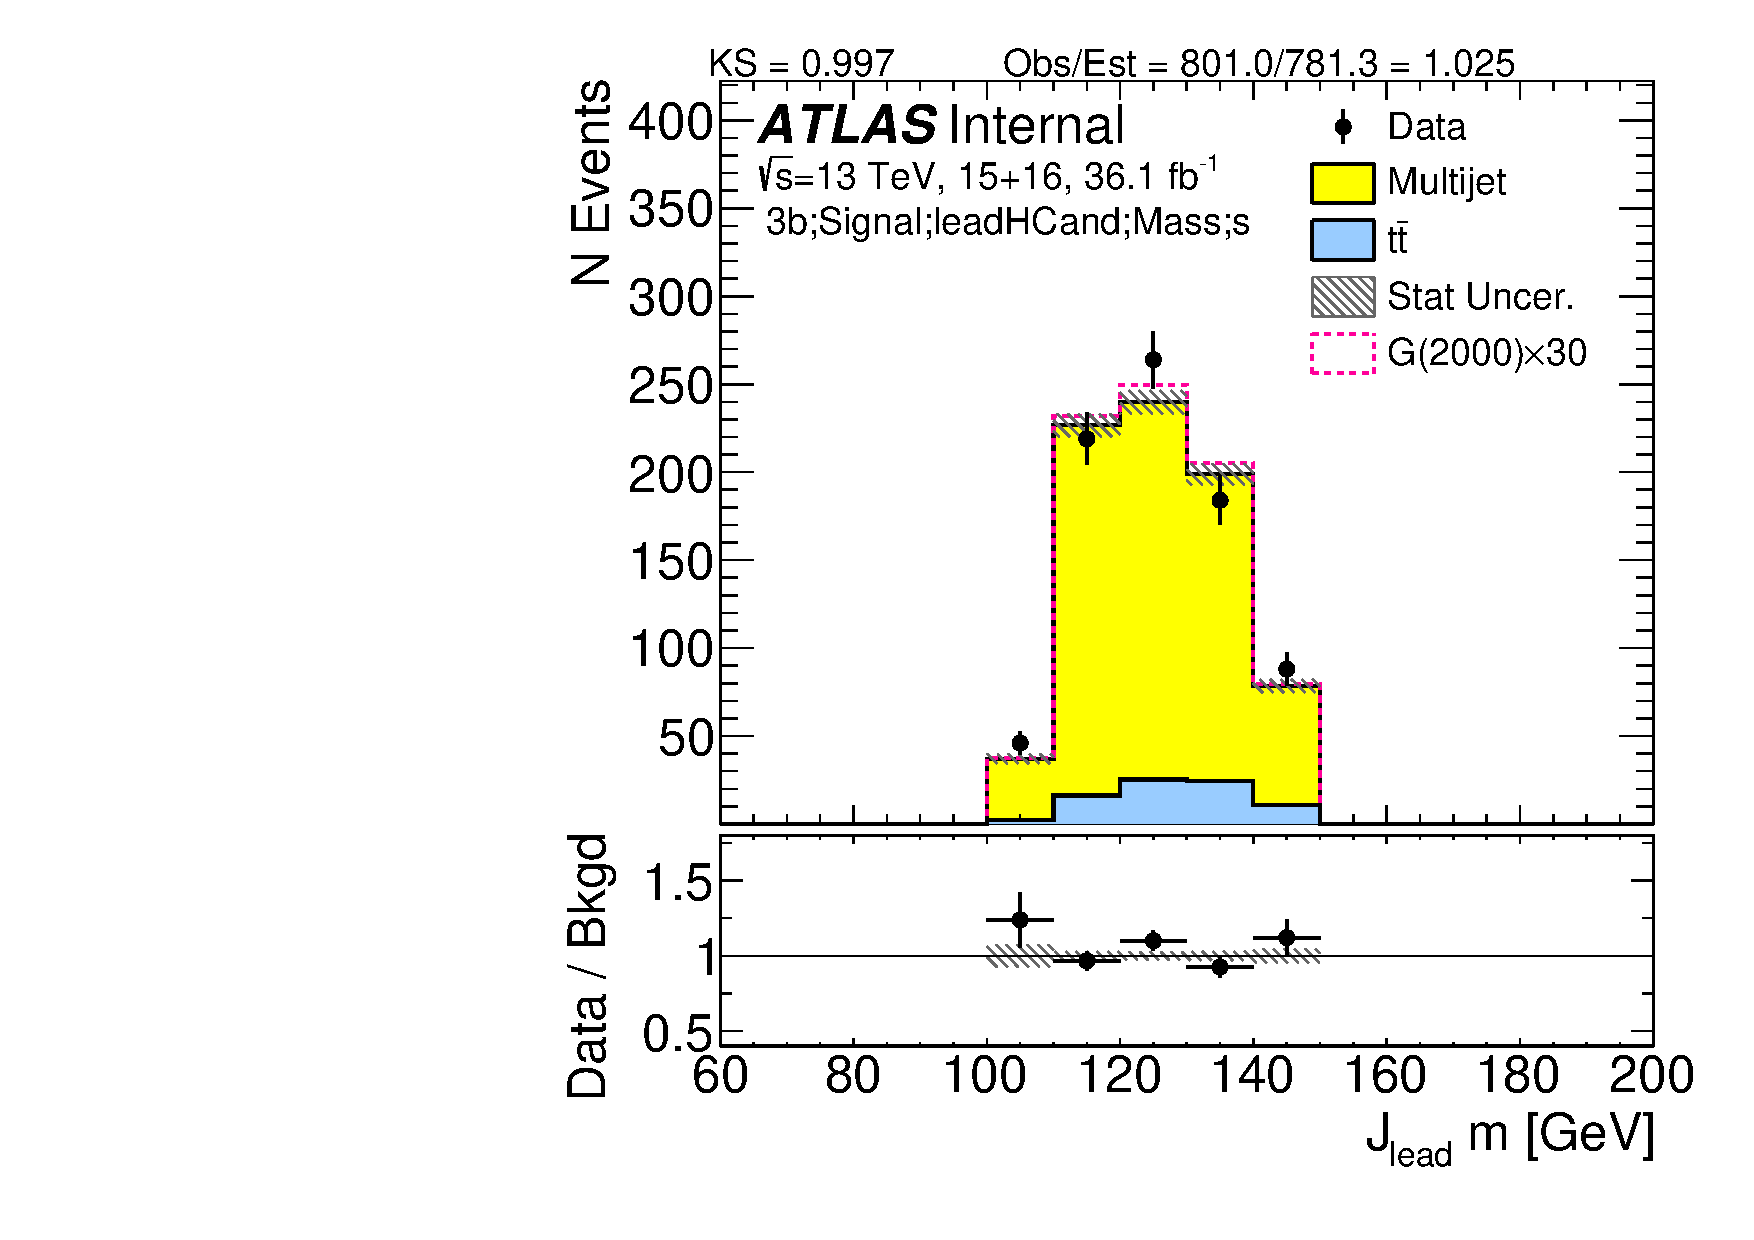
\includegraphics[width=0.31\textwidth,angle=-90]{figures/boosted/Signal/b77_ThreeTag_Signal_leadHCand_Mass_s.pdf}\\
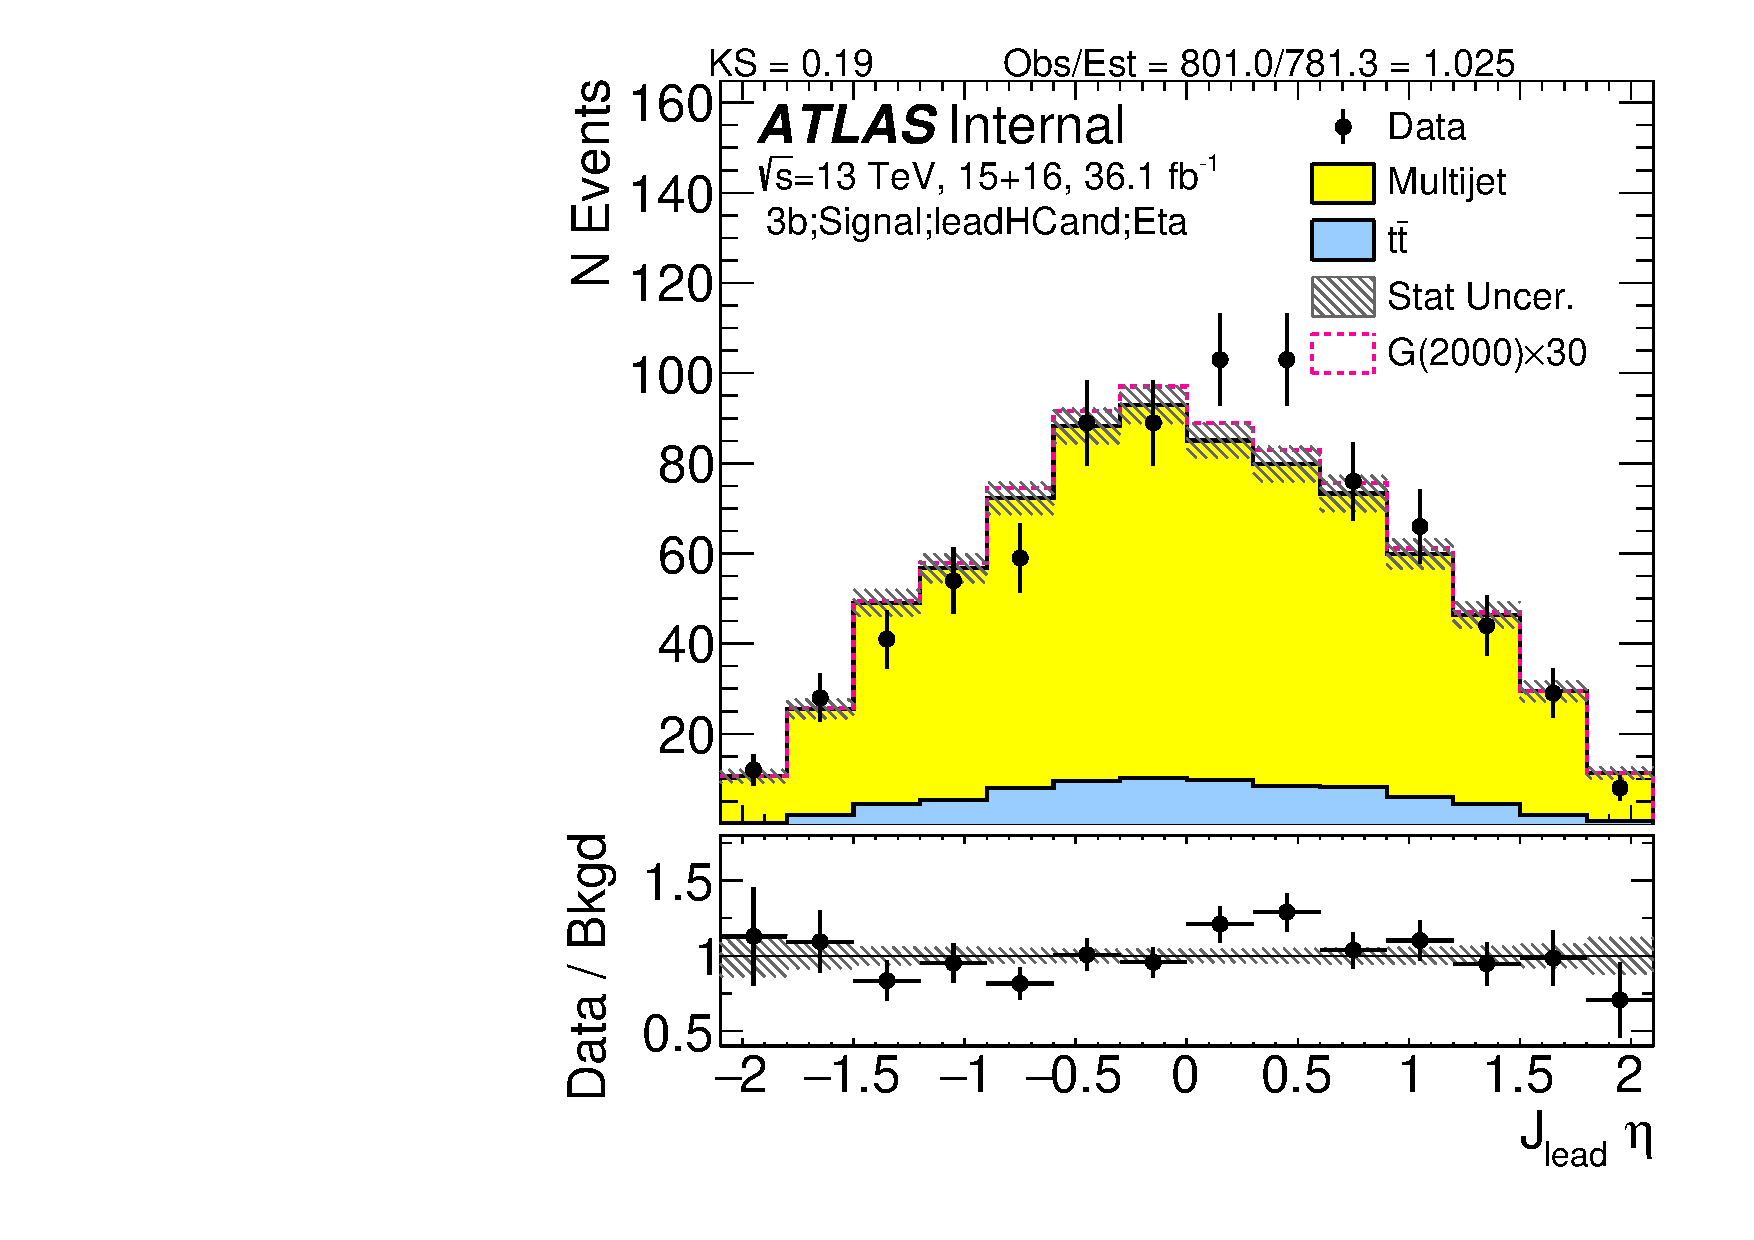
\includegraphics[width=0.31\textwidth,angle=-90]{figures/boosted/Signal/b77_ThreeTag_Signal_leadHCand_Eta.pdf}
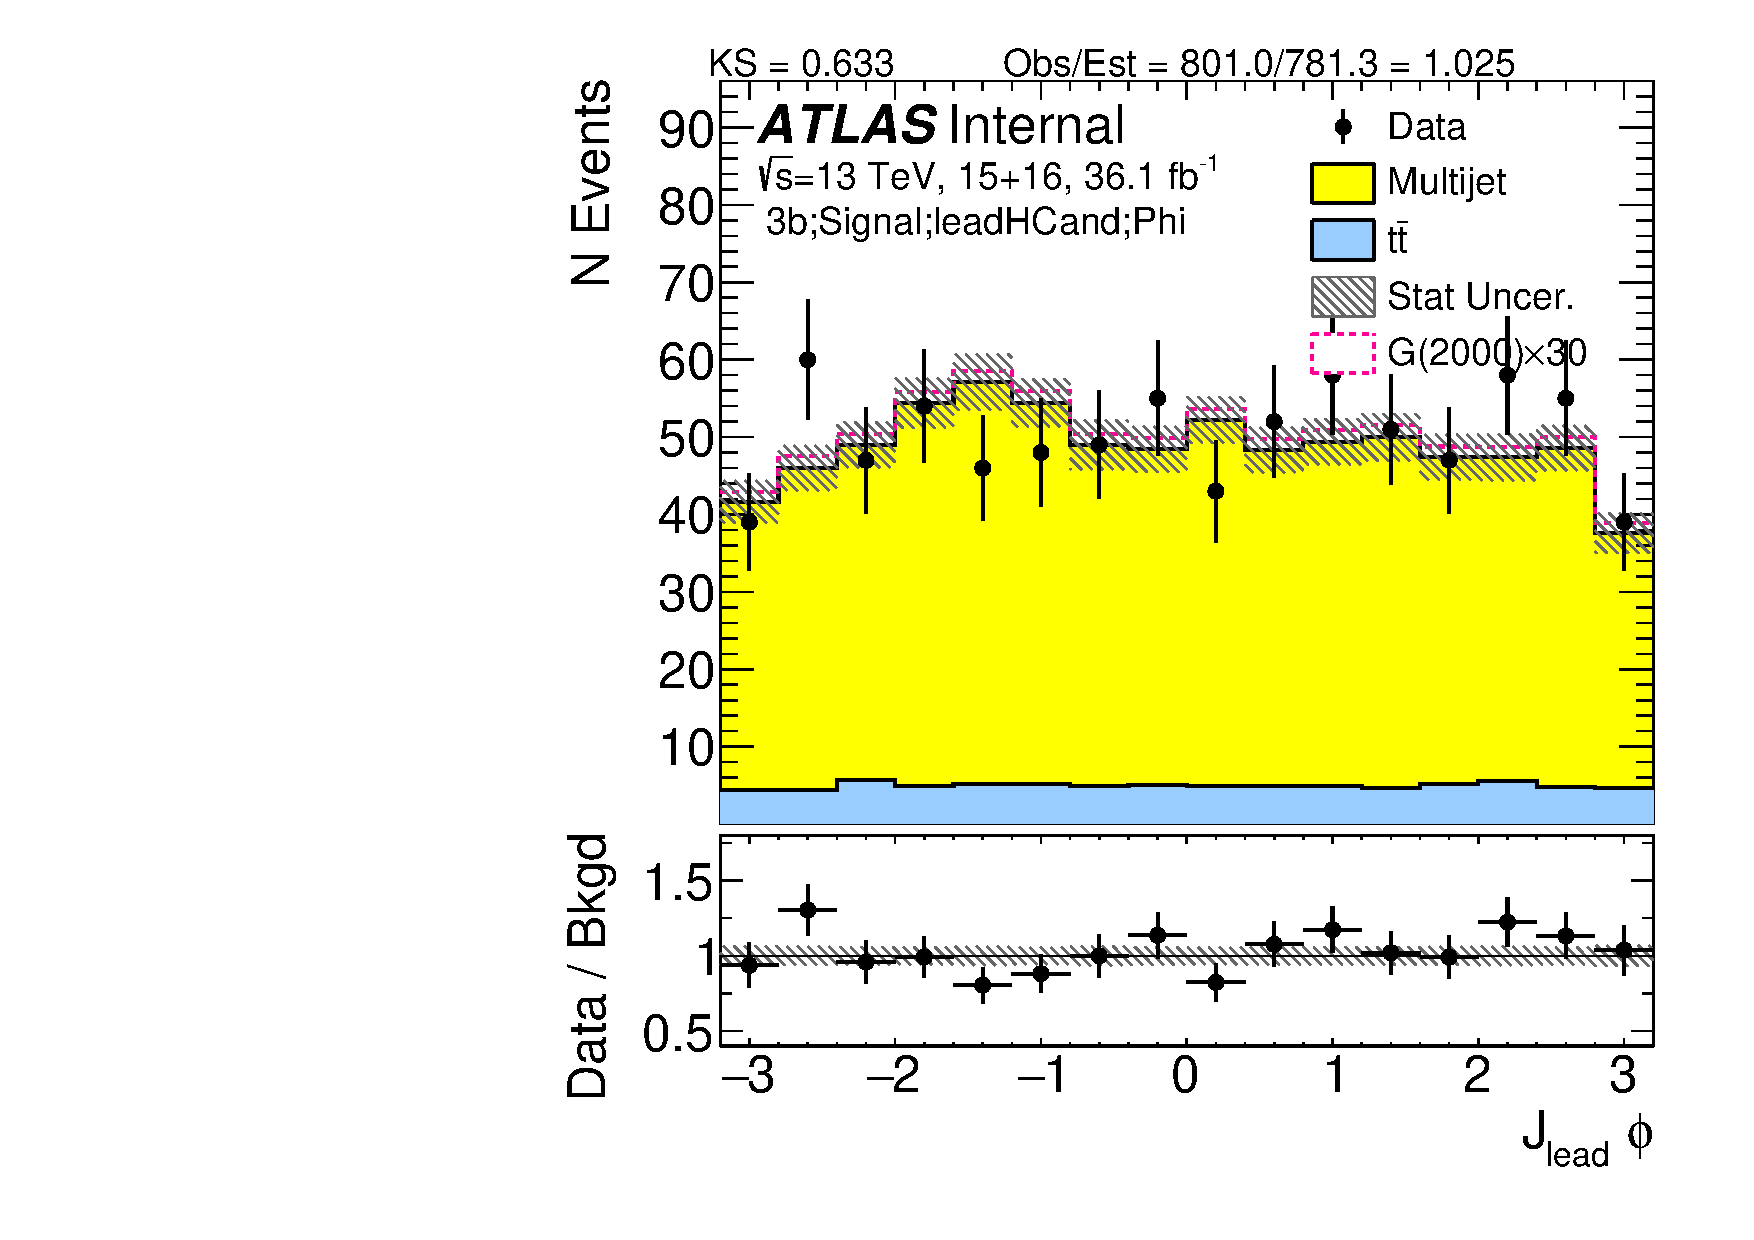
\includegraphics[width=0.31\textwidth,angle=-90]{figures/boosted/Signal/b77_ThreeTag_Signal_leadHCand_Phi.pdf}
  \caption{Kinematics (\pt~, mass, $\eta$, $\phi$) of the lead large-\R jet in data and prediction in the signal region after requiring 3 $b$-tags. }
  \label{fig:boosted-3b-signal-ak10-lead}
\end{center}
\end{figure*}

\begin{figure*}[htbp!]
\begin{center}
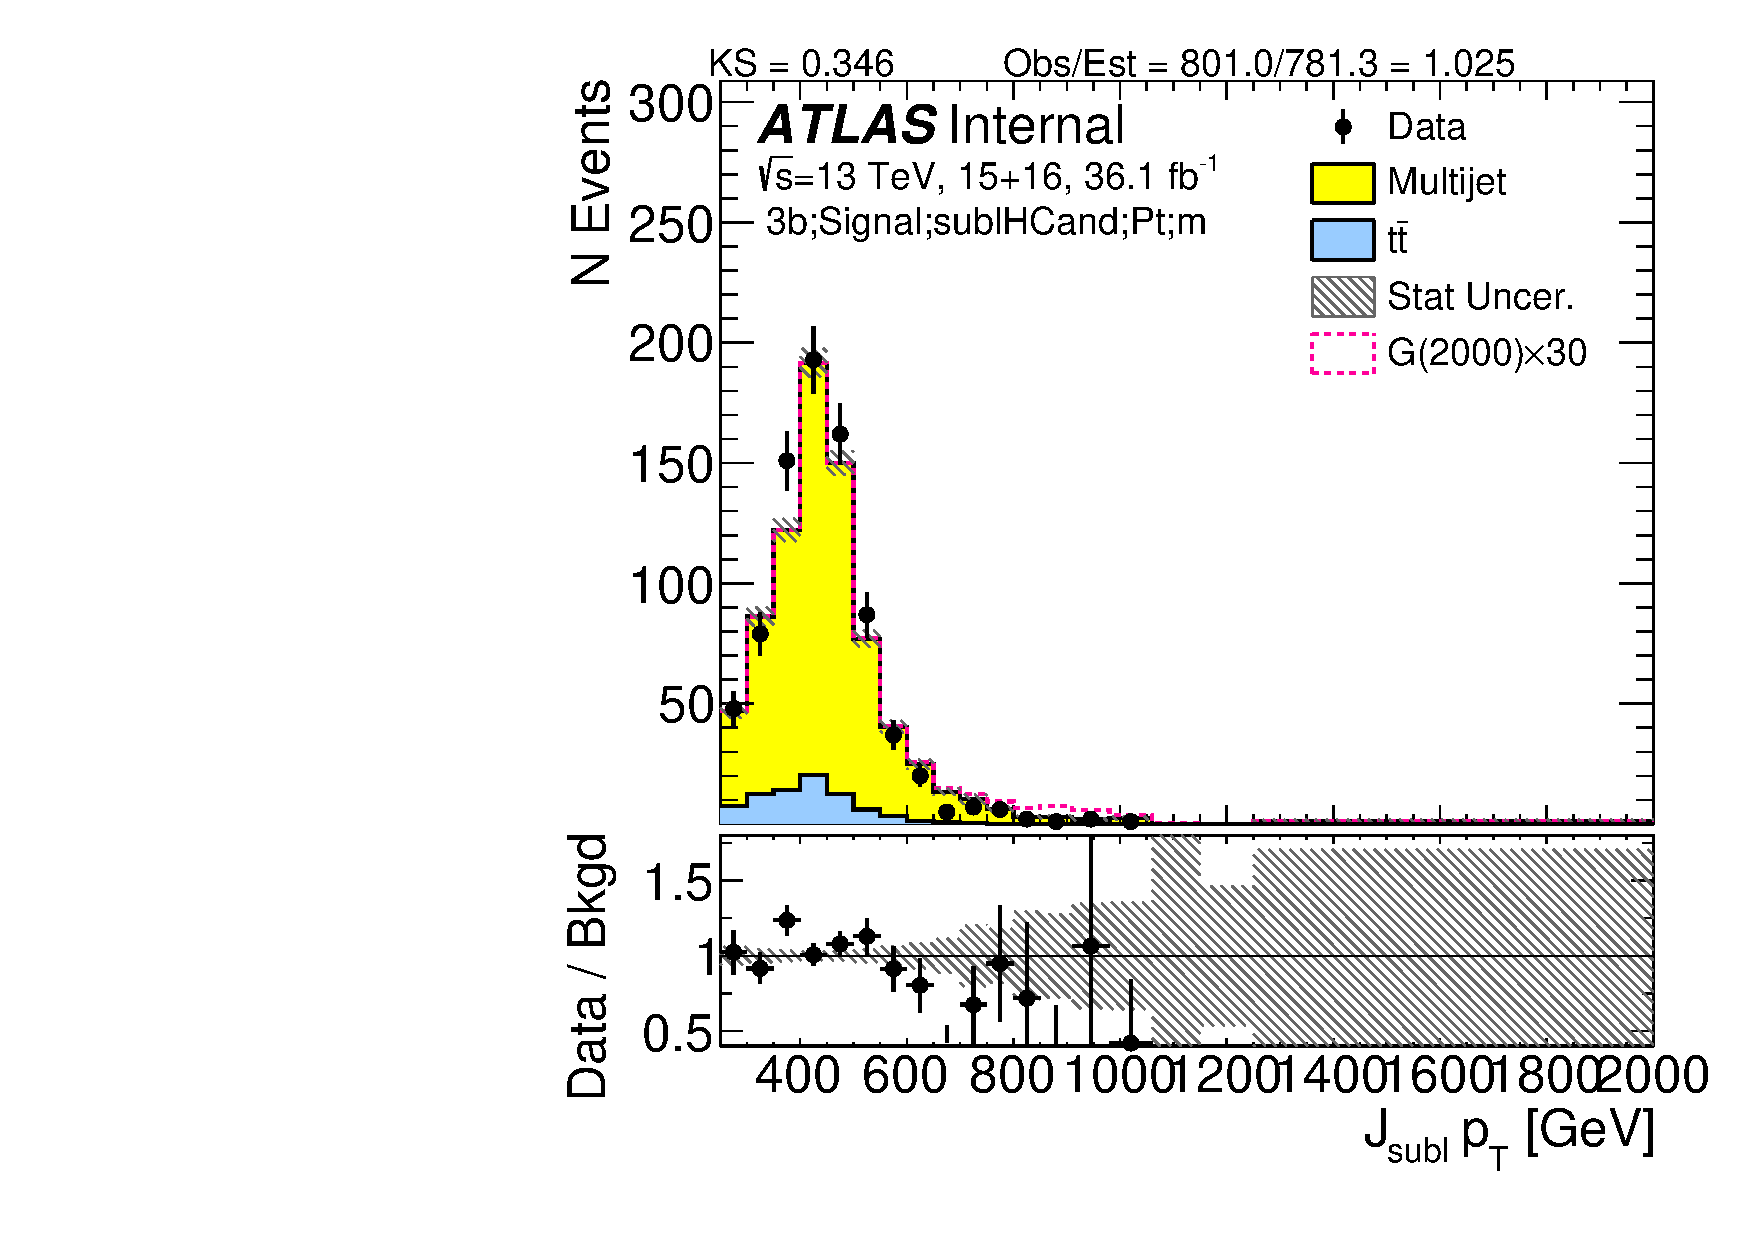
\includegraphics[width=0.31\textwidth,angle=-90]{figures/boosted/Signal/b77_ThreeTag_Signal_sublHCand_Pt_m.pdf}
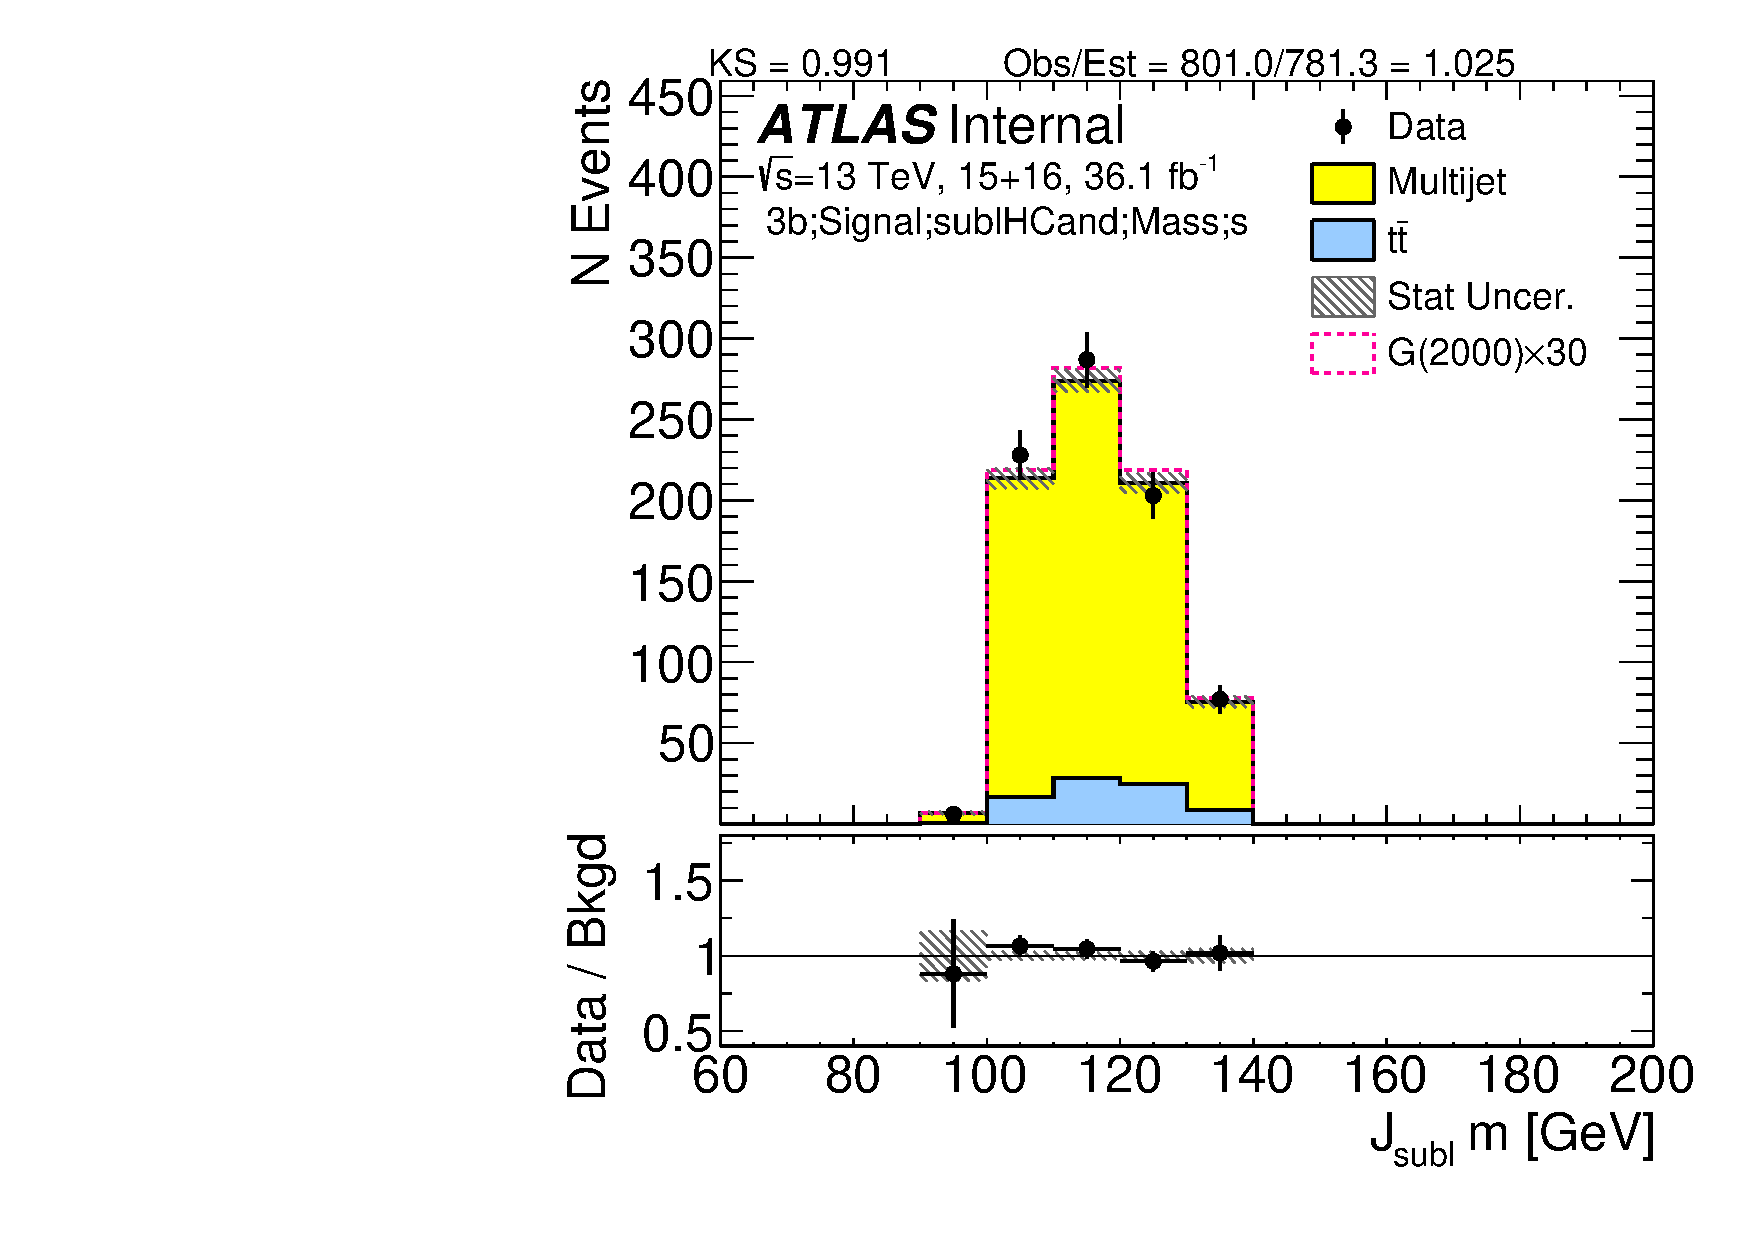
\includegraphics[width=0.31\textwidth,angle=-90]{figures/boosted/Signal/b77_ThreeTag_Signal_sublHCand_Mass_s.pdf}\\
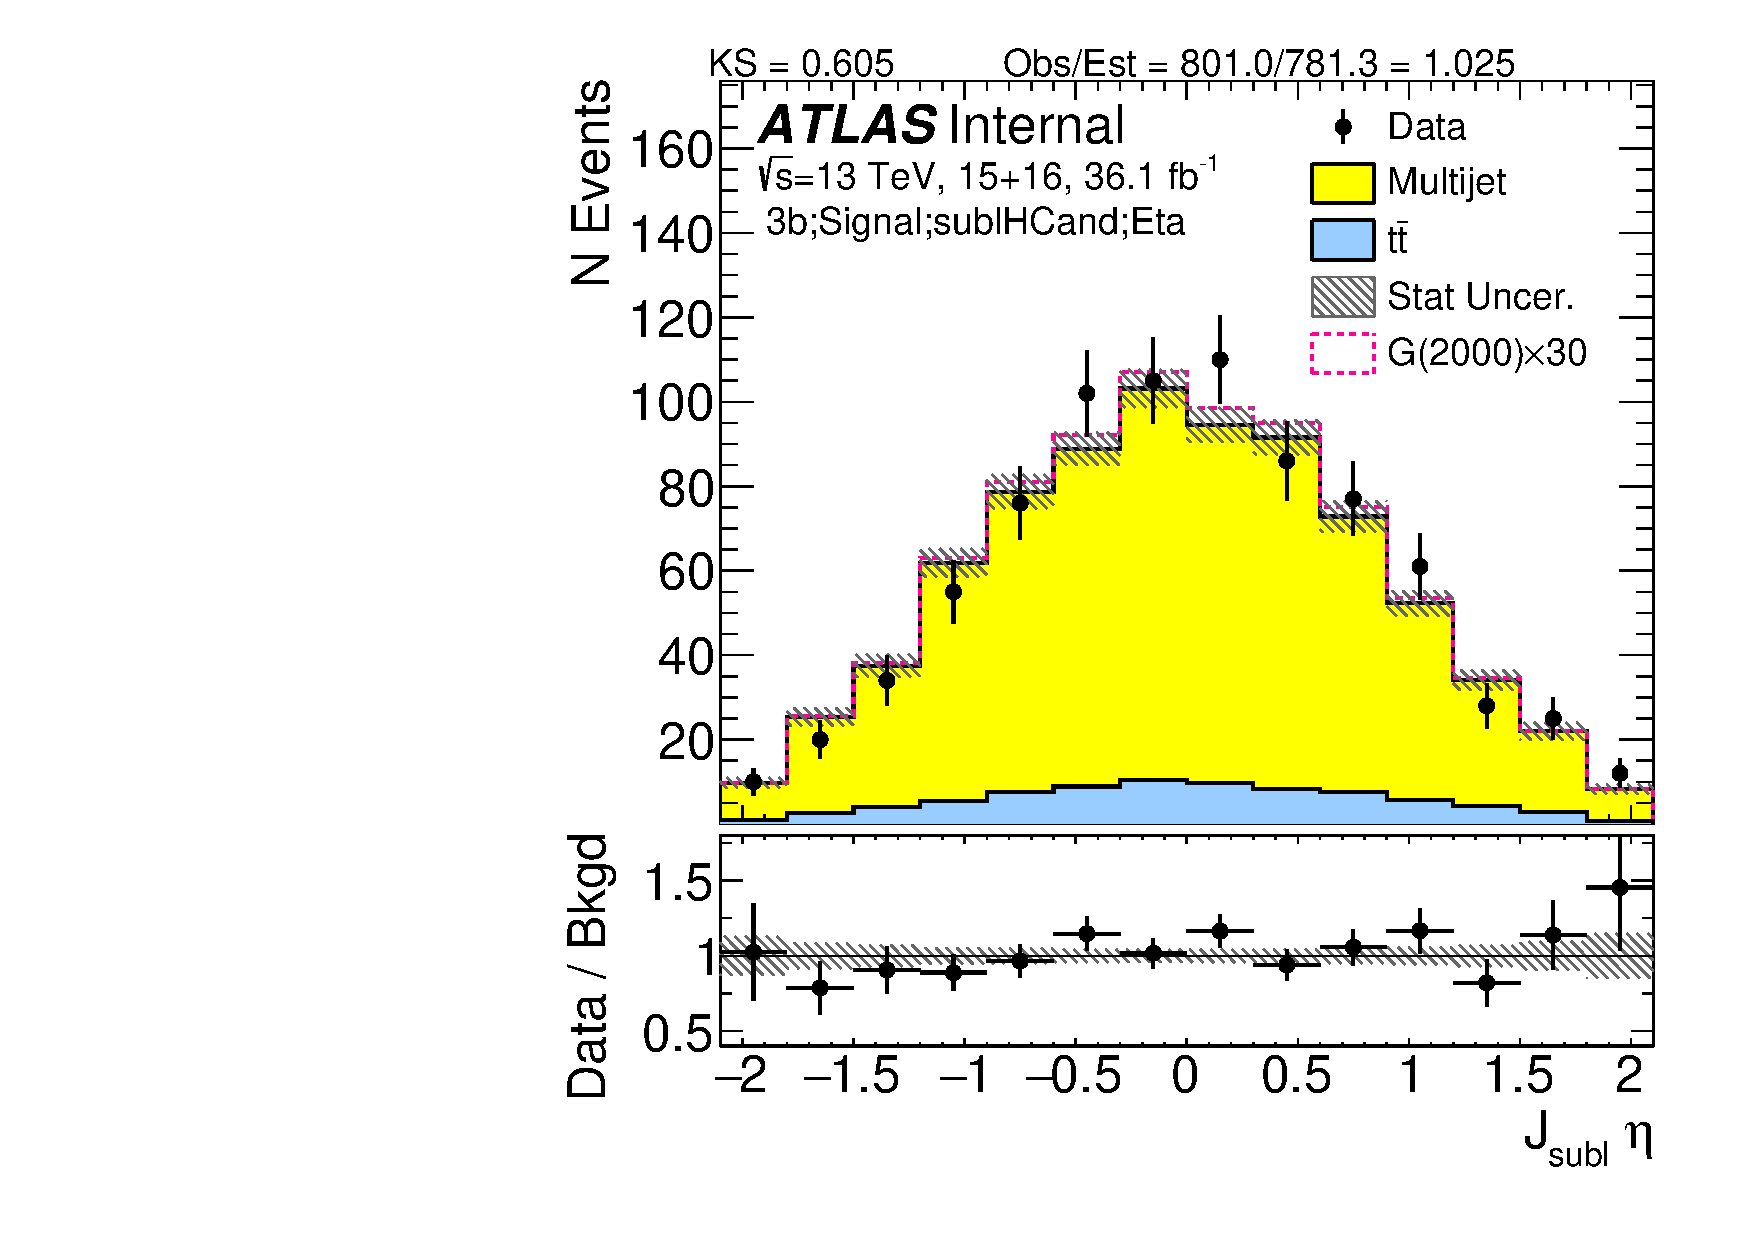
\includegraphics[width=0.31\textwidth,angle=-90]{figures/boosted/Signal/b77_ThreeTag_Signal_sublHCand_Eta.pdf}
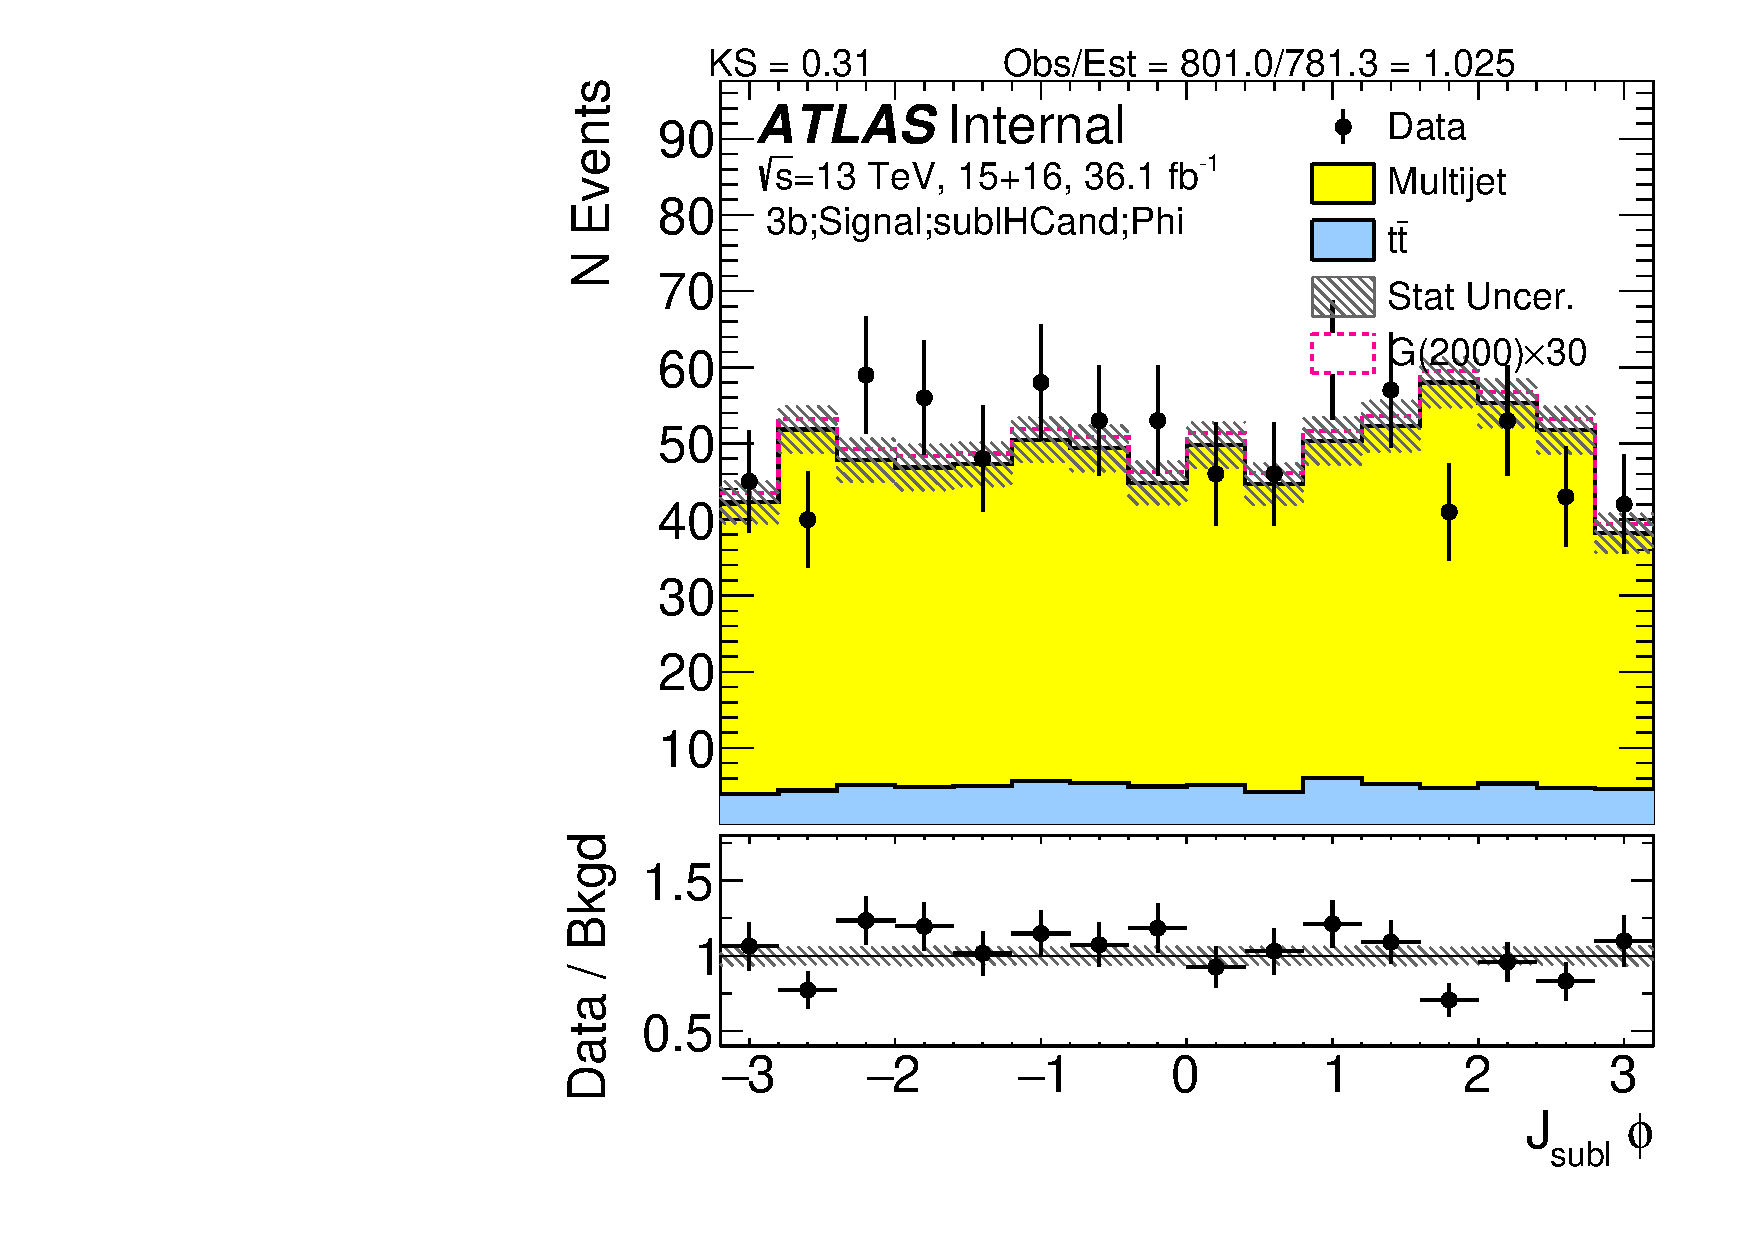
\includegraphics[width=0.31\textwidth,angle=-90]{figures/boosted/Signal/b77_ThreeTag_Signal_sublHCand_Phi.pdf}
  \caption{Kinematics (\pt~, mass, $\eta$, $\phi$) of the subleading large-\R jet in data and prediction in the signal region after requiring 3 $b$-tags. }
  \label{fig:boosted-3b-signal-ak10-subl}
\end{center}
\end{figure*}

\begin{figure*}[htbp!]
\begin{center}
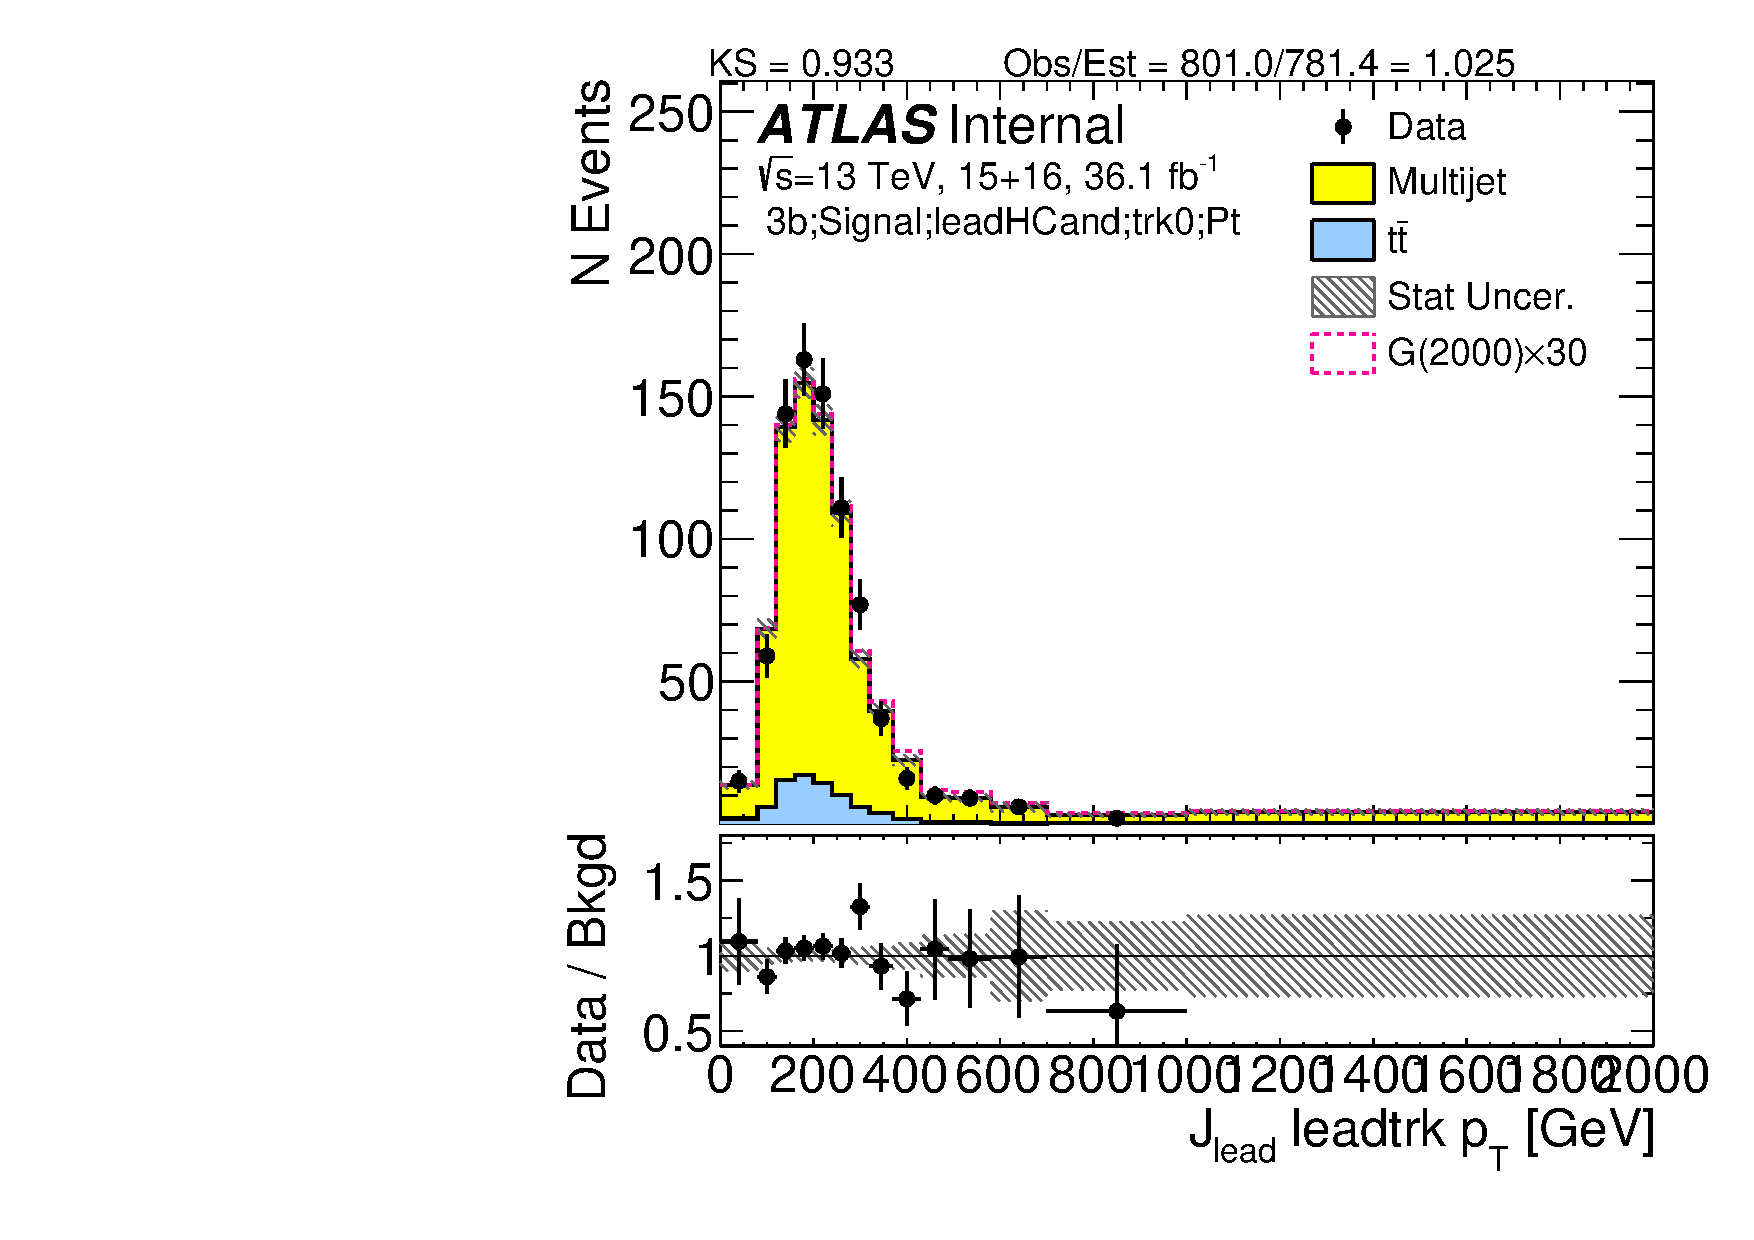
\includegraphics[width=0.31\textwidth,angle=-90]{figures/boosted/Signal/b77_ThreeTag_Signal_leadHCand_trk0_Pt.pdf}
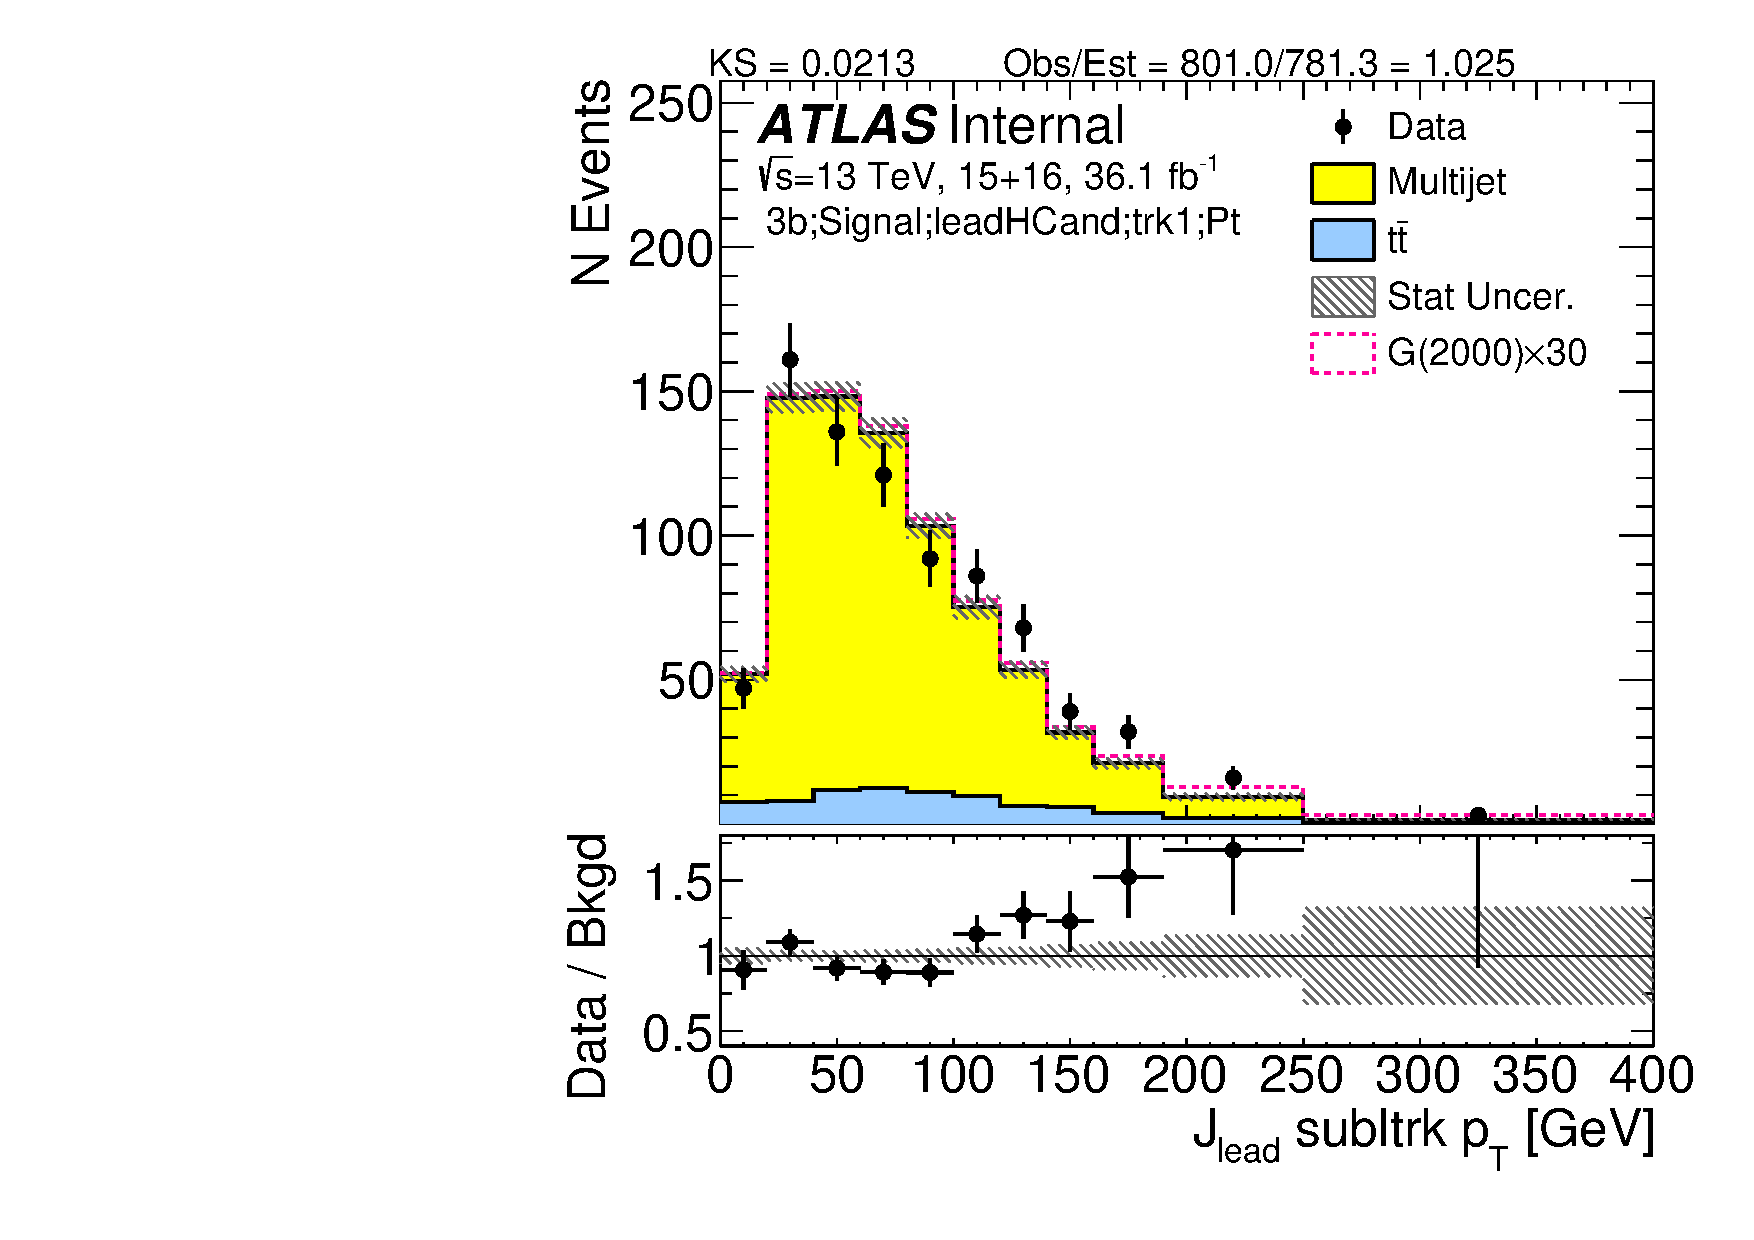
\includegraphics[width=0.31\textwidth,angle=-90]{figures/boosted/Signal/b77_ThreeTag_Signal_leadHCand_trk1_Pt.pdf}\\
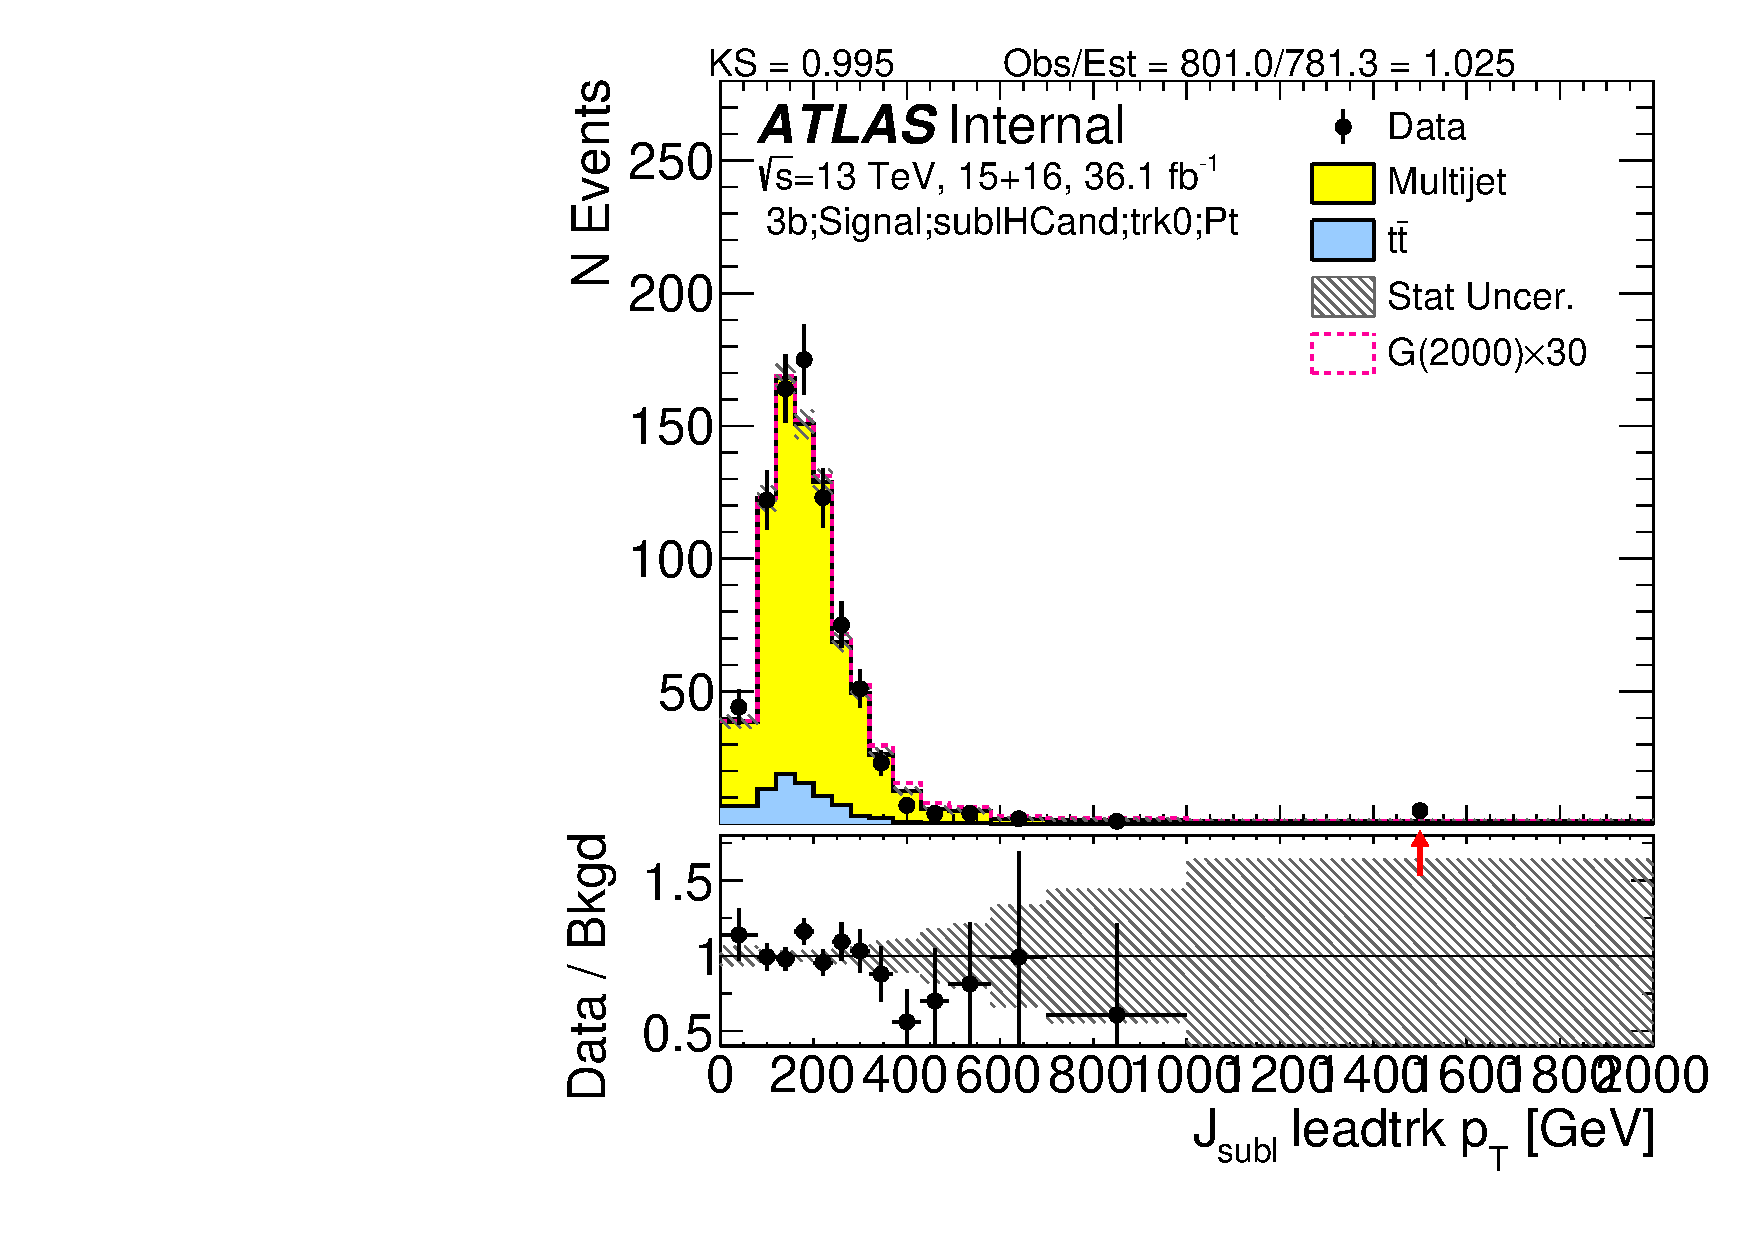
\includegraphics[width=0.31\textwidth,angle=-90]{figures/boosted/Signal/b77_ThreeTag_Signal_sublHCand_trk0_Pt.pdf}
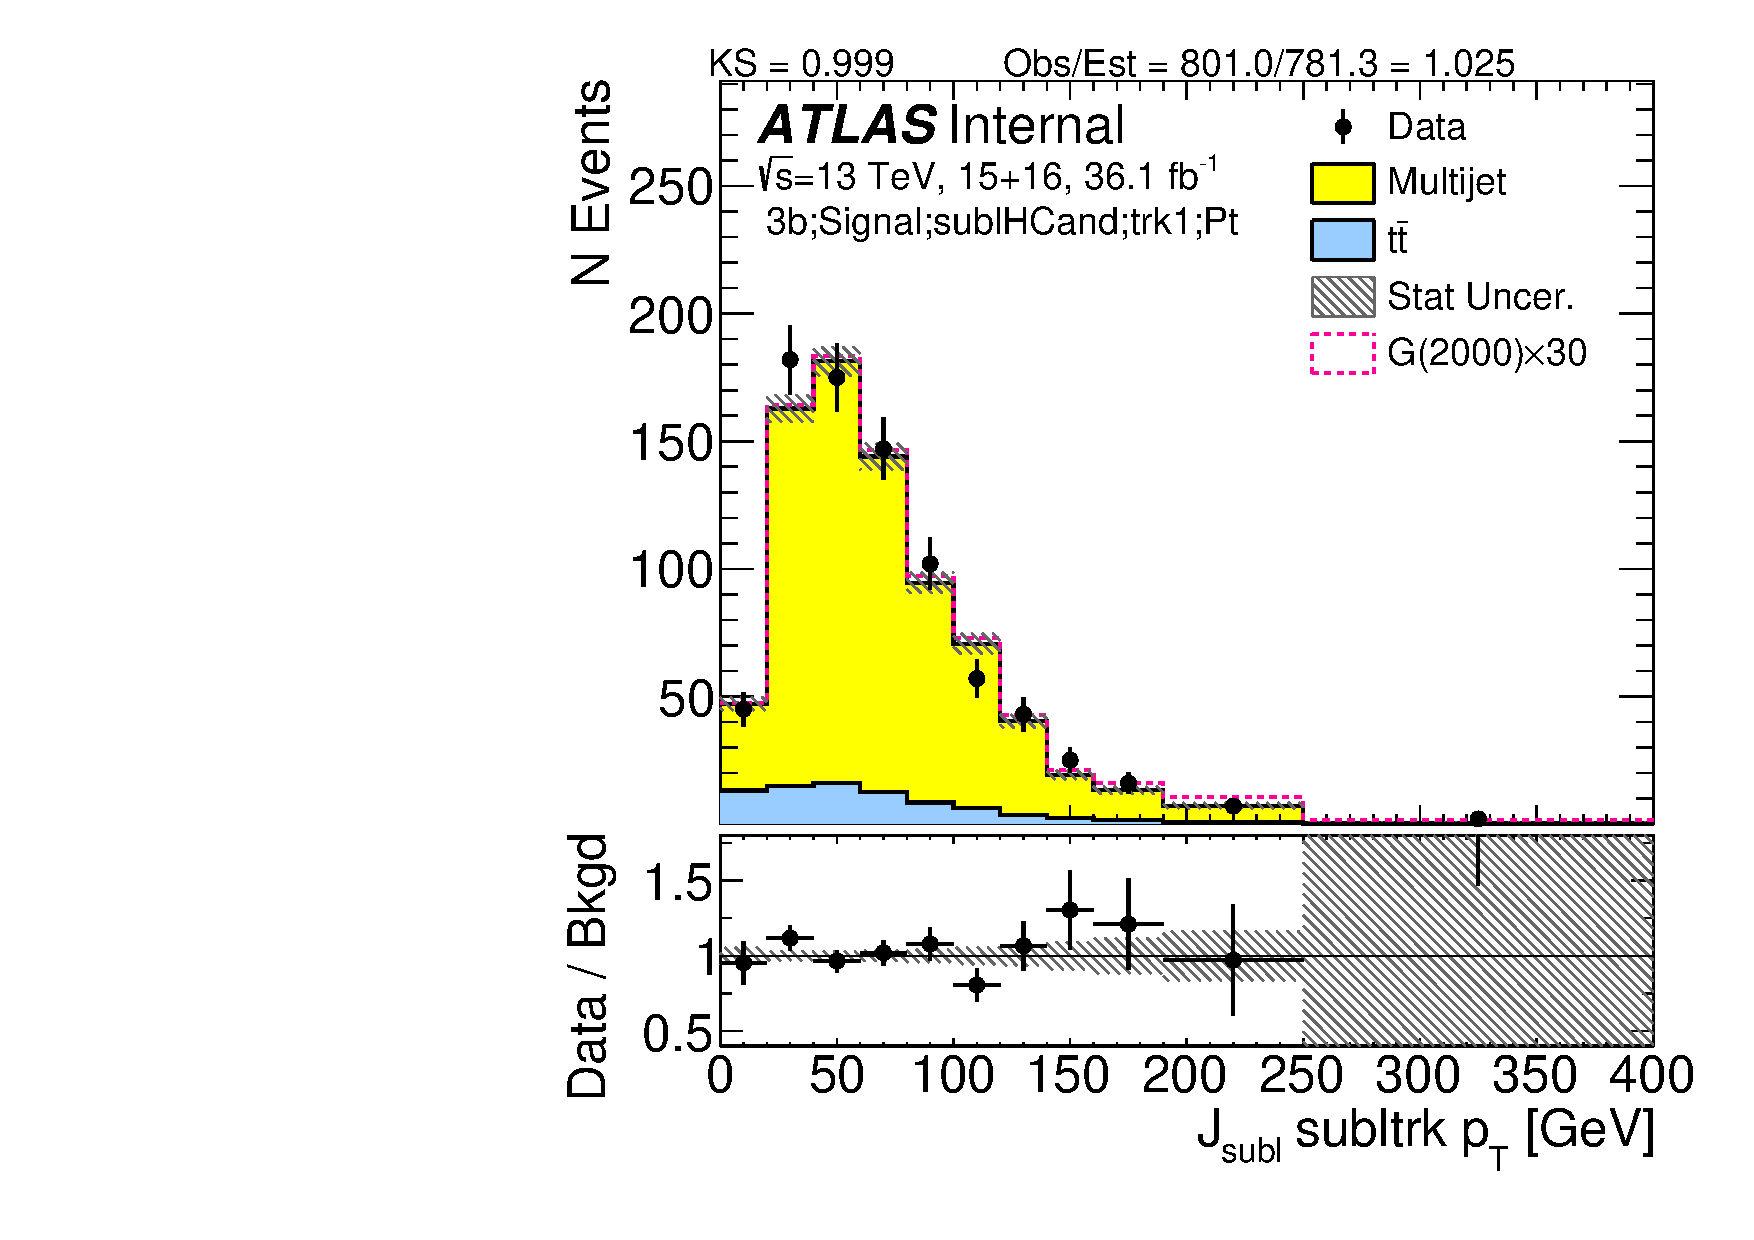
\includegraphics[width=0.31\textwidth,angle=-90]{figures/boosted/Signal/b77_ThreeTag_Signal_sublHCand_trk1_Pt.pdf}\\
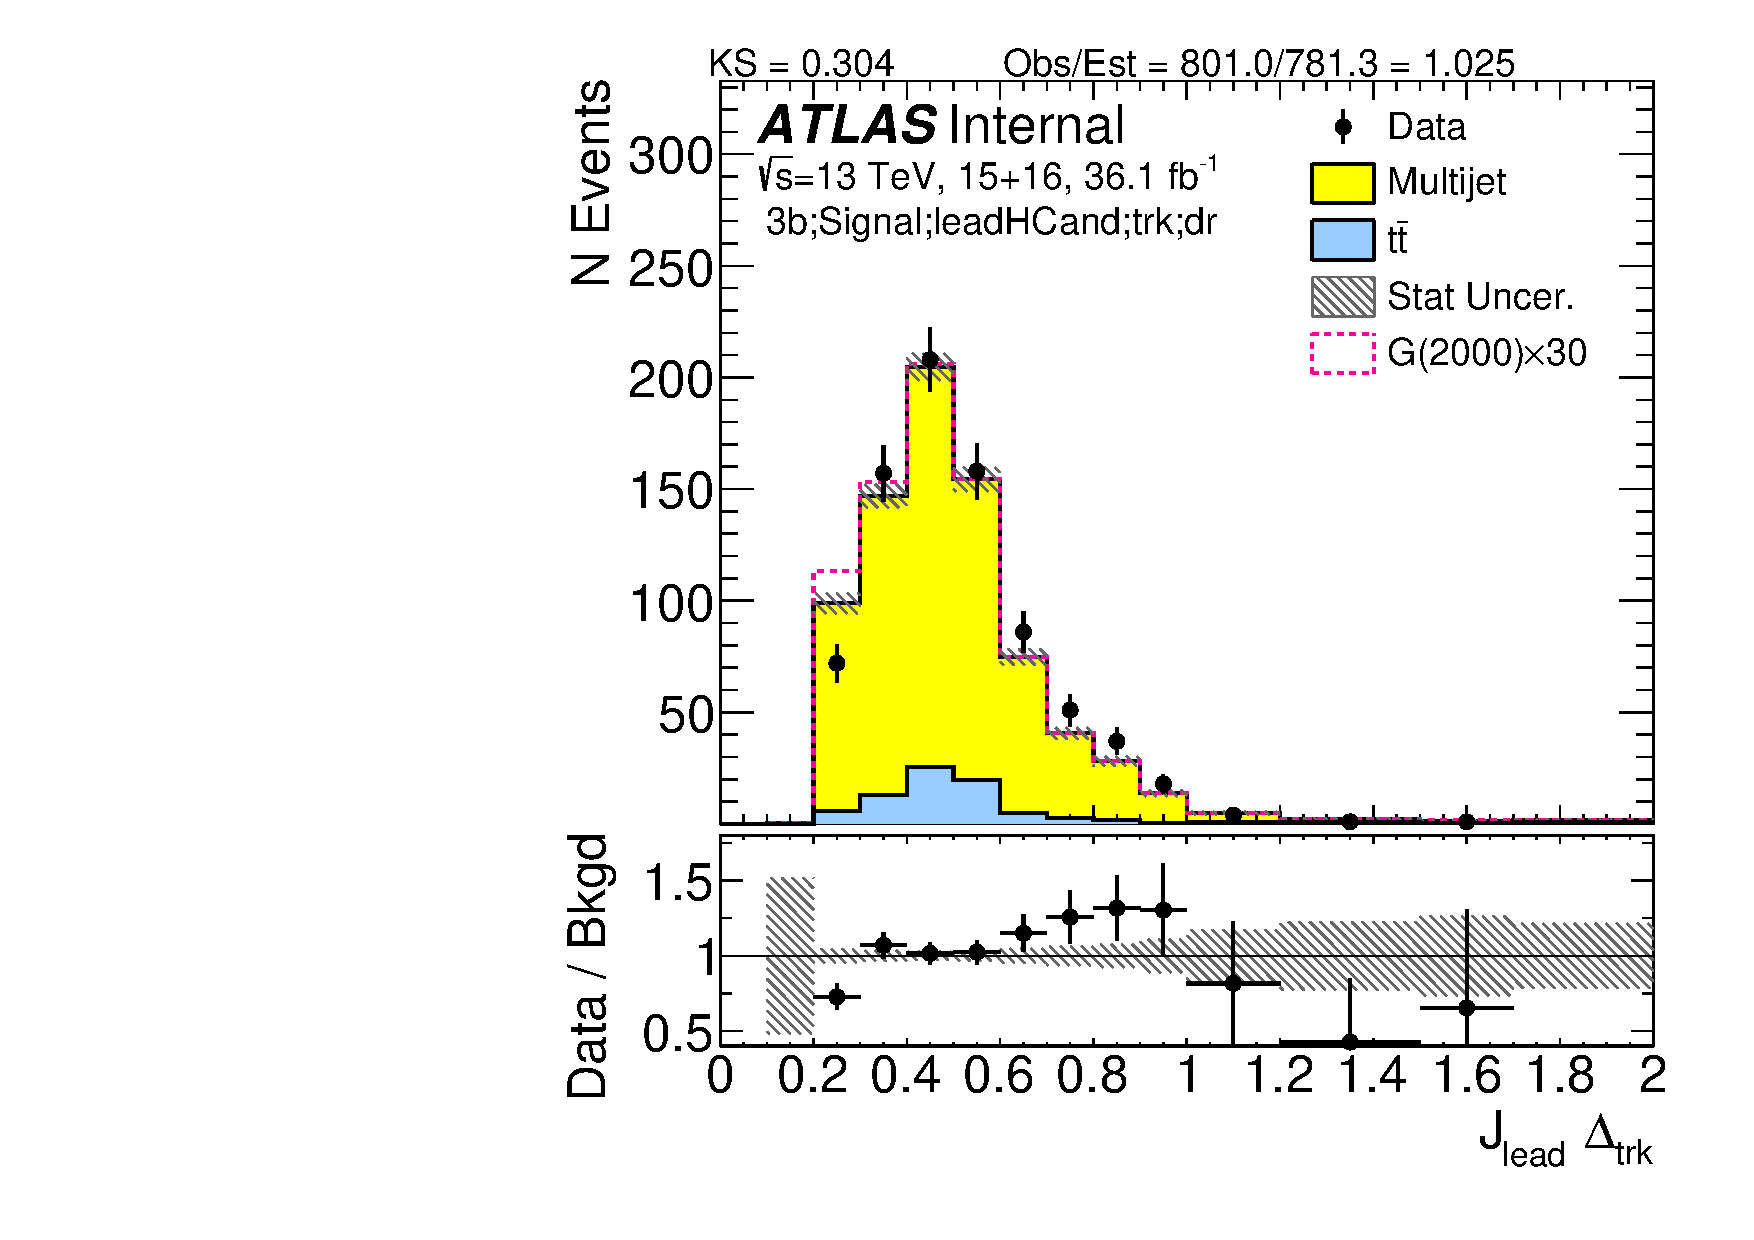
\includegraphics[width=0.31\textwidth,angle=-90]{figures/boosted/Signal/b77_ThreeTag_Signal_leadHCand_trk_dr.pdf}
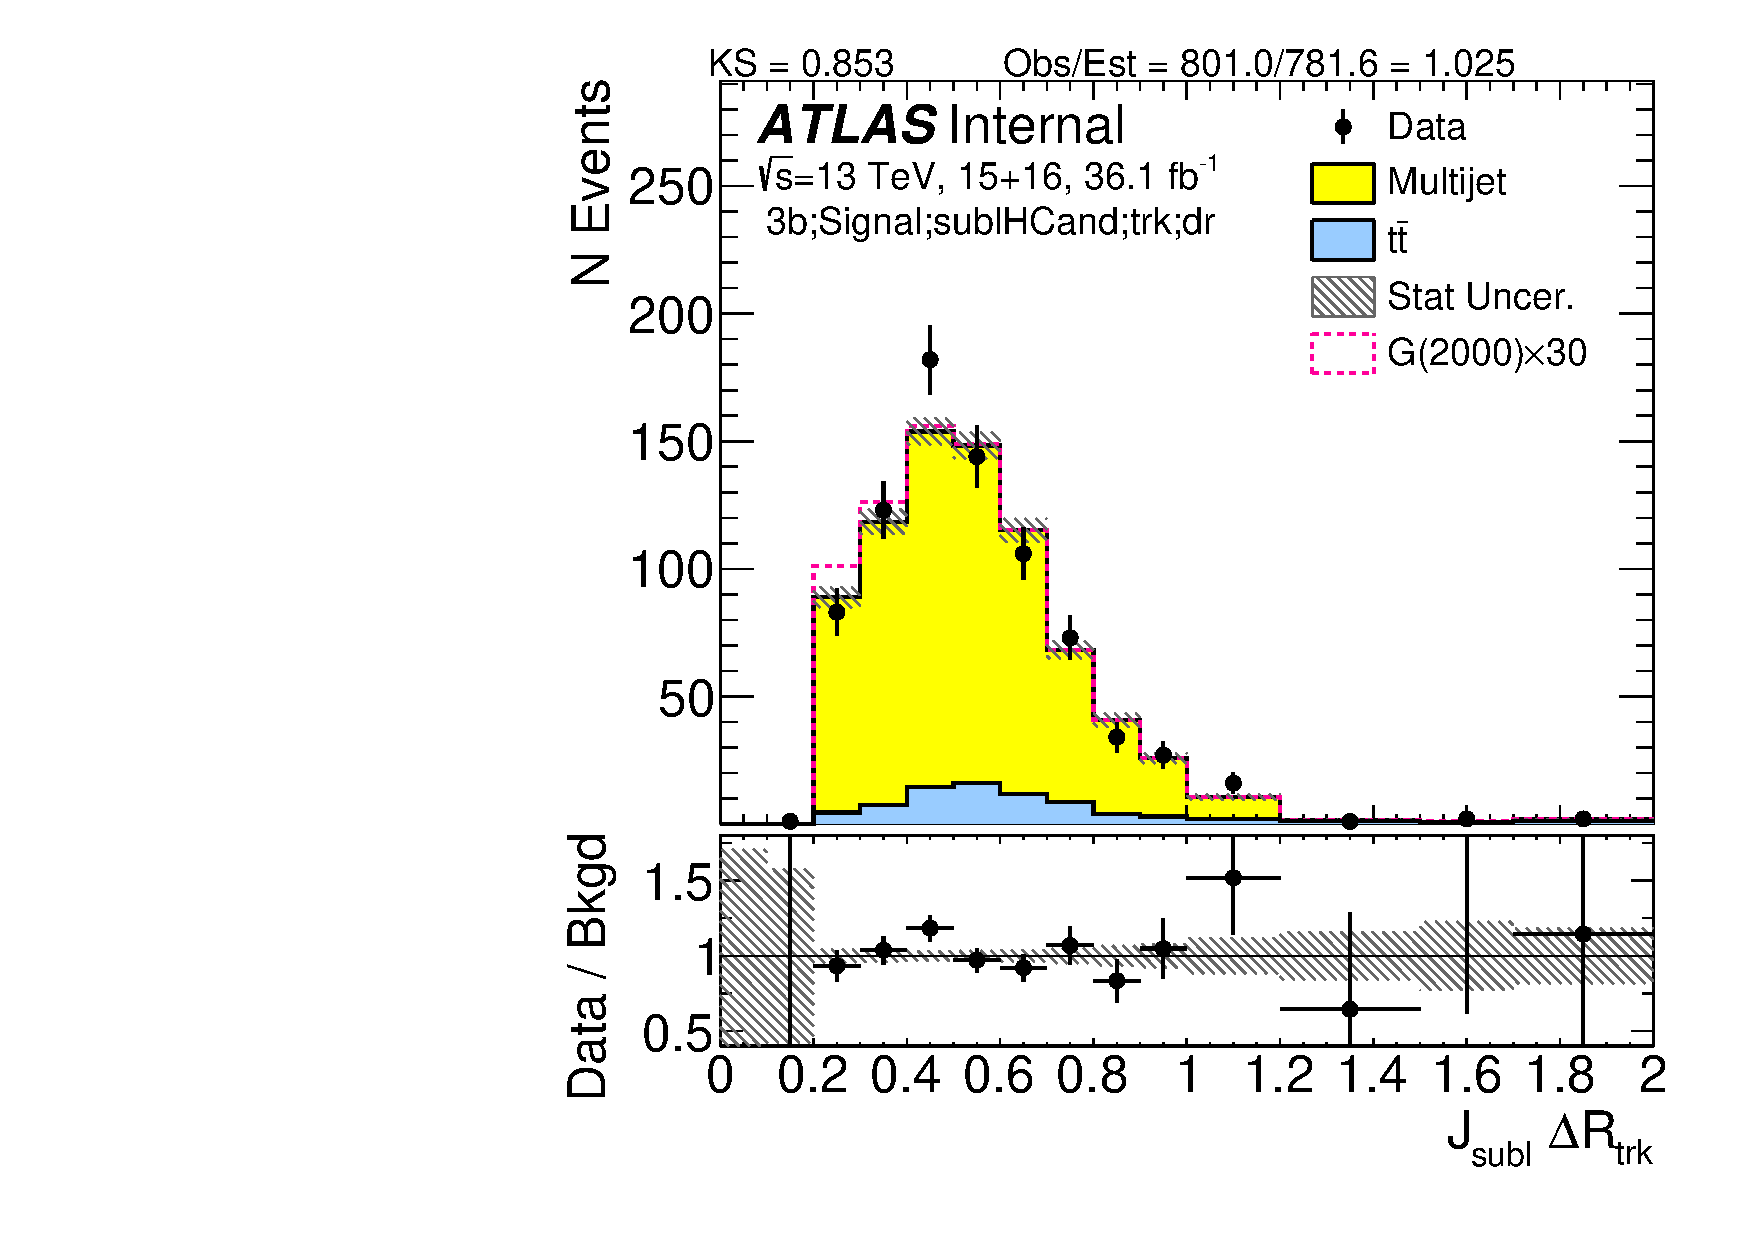
\includegraphics[width=0.31\textwidth,angle=-90]{figures/boosted/Signal/b77_ThreeTag_Signal_sublHCand_trk_dr.pdf}
  \caption{First two rows show the \pt~ of the lead (left) and sub-lead (right) small-$R$ track jets associated to the lead (first-row) and sub-lead (second-row) large-\R jet in data and prediction in the signal region after requiring 3 $b$-tags. Third row shows the $\Delta R$ between two leading small-$R$ track-jets associated to the leading (left) and sub-leading (right) large-\R jet.  }
  \label{fig:boosted-3b-signal-ak2}
\end{center}
\end{figure*}


\begin{figure*}[htbp!]
\begin{center}
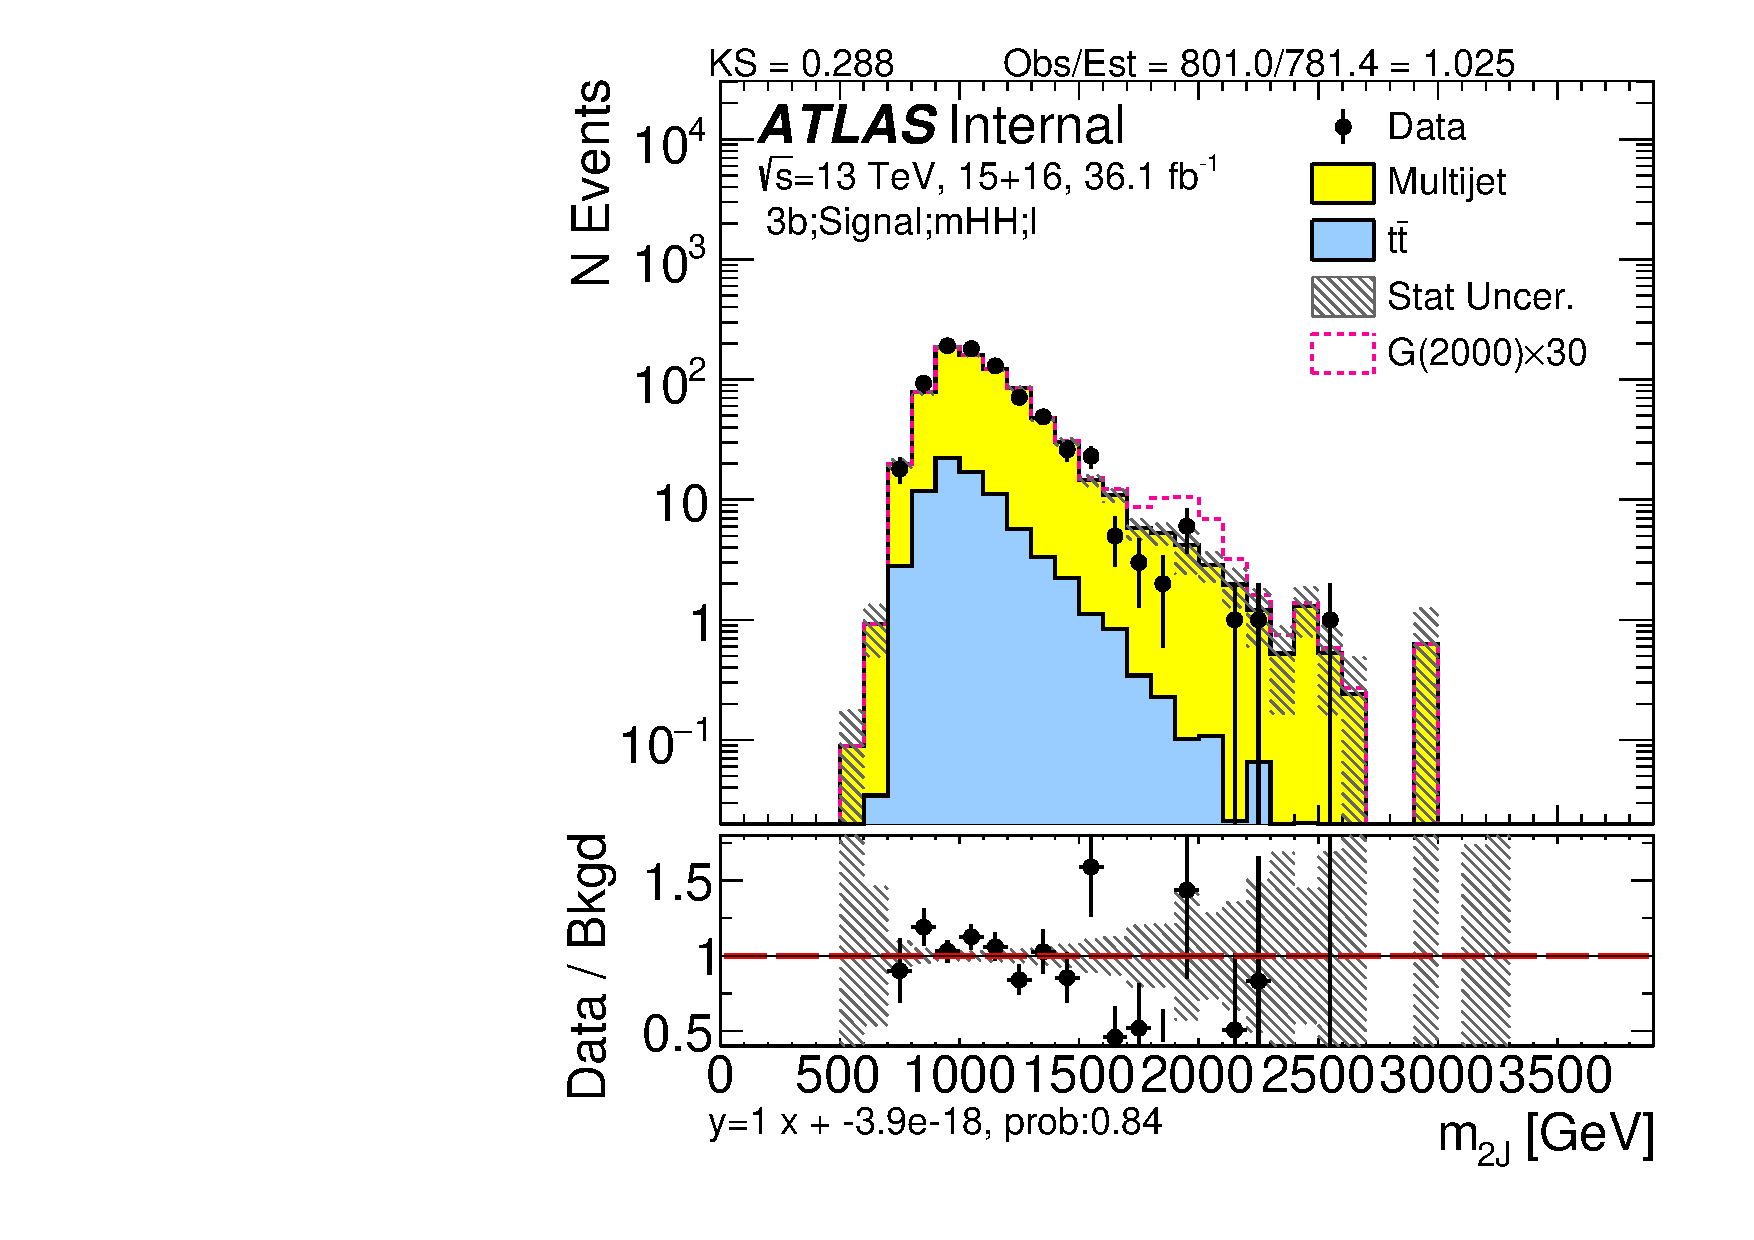
\includegraphics[width=0.31\textwidth,angle=-90]{figures/boosted/Signal/b77_ThreeTag_Signal_mHH_l_1.pdf}
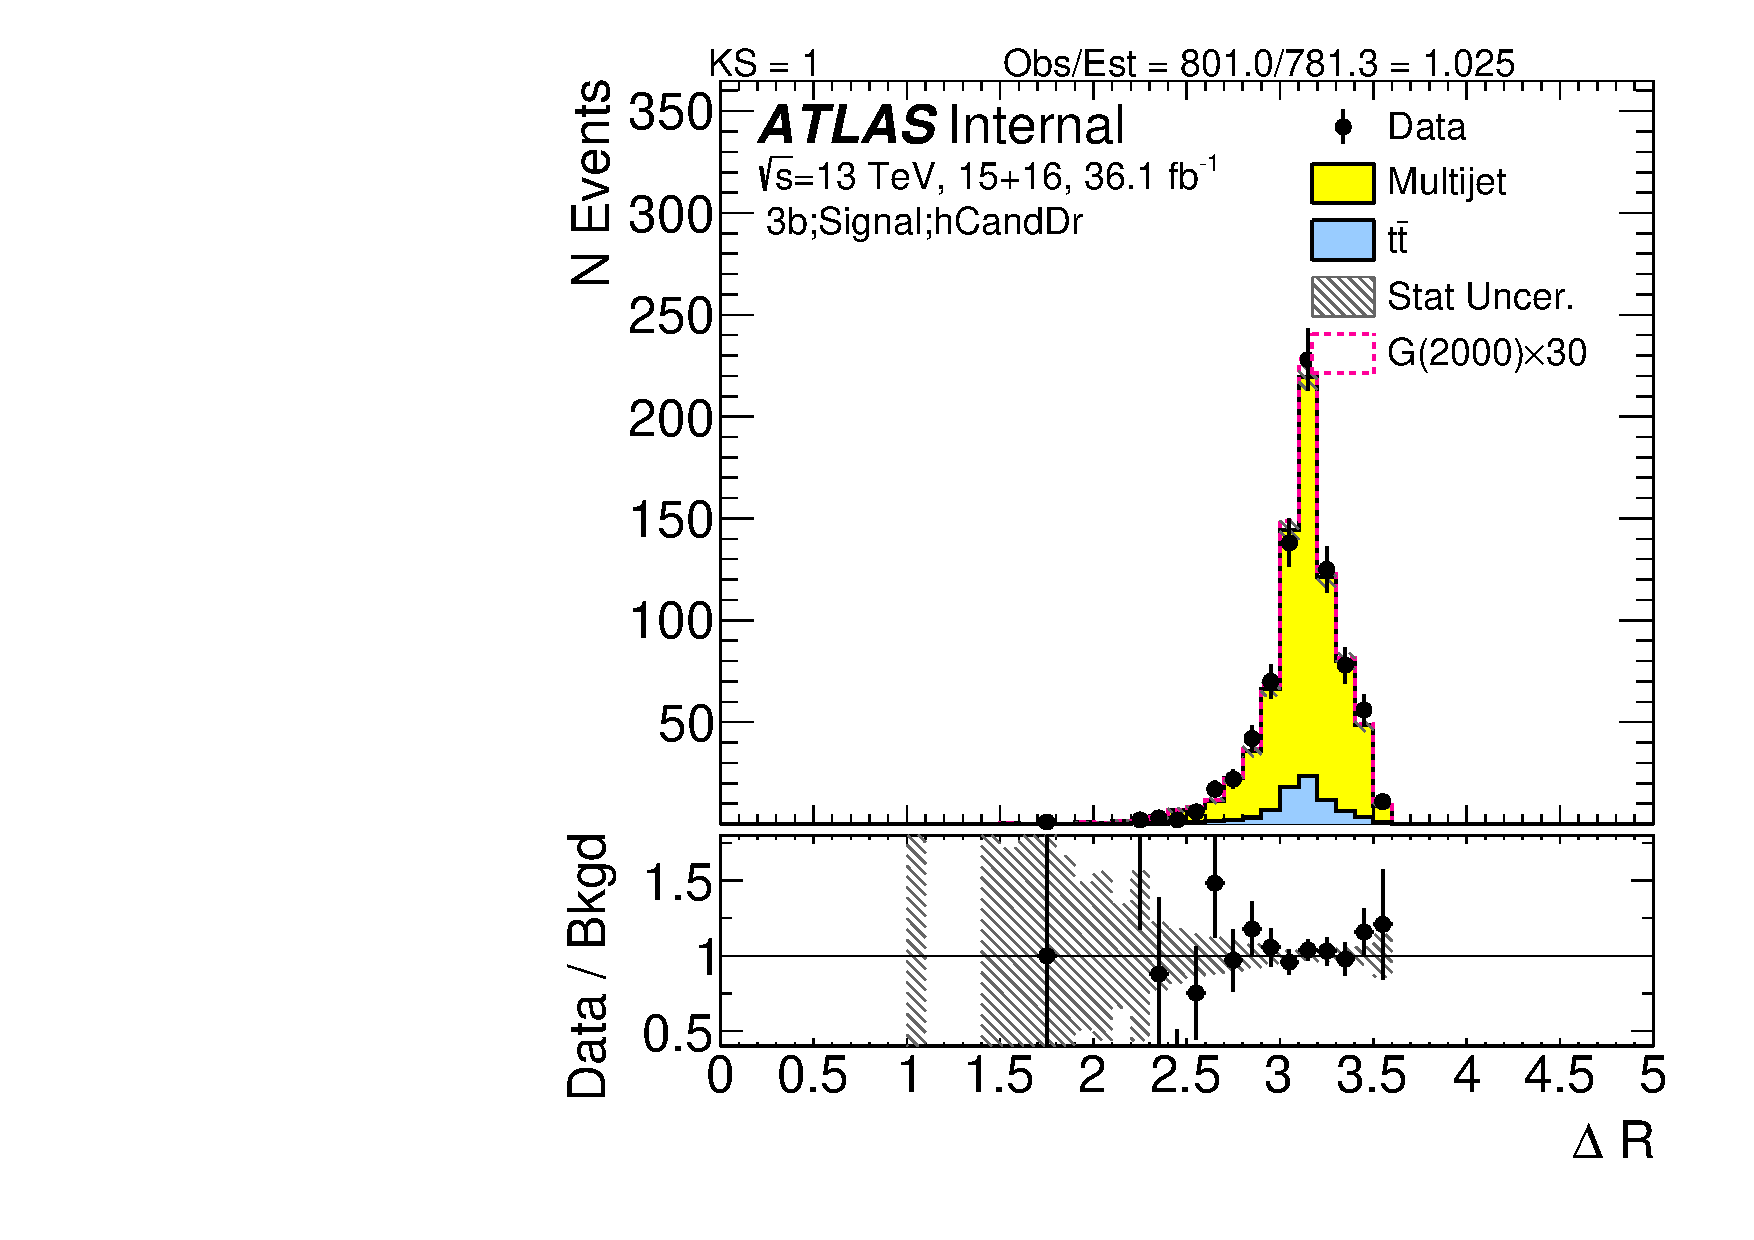
\includegraphics[width=0.31\textwidth,angle=-90]{figures/boosted/Signal/b77_ThreeTag_Signal_hCandDr.pdf}\\
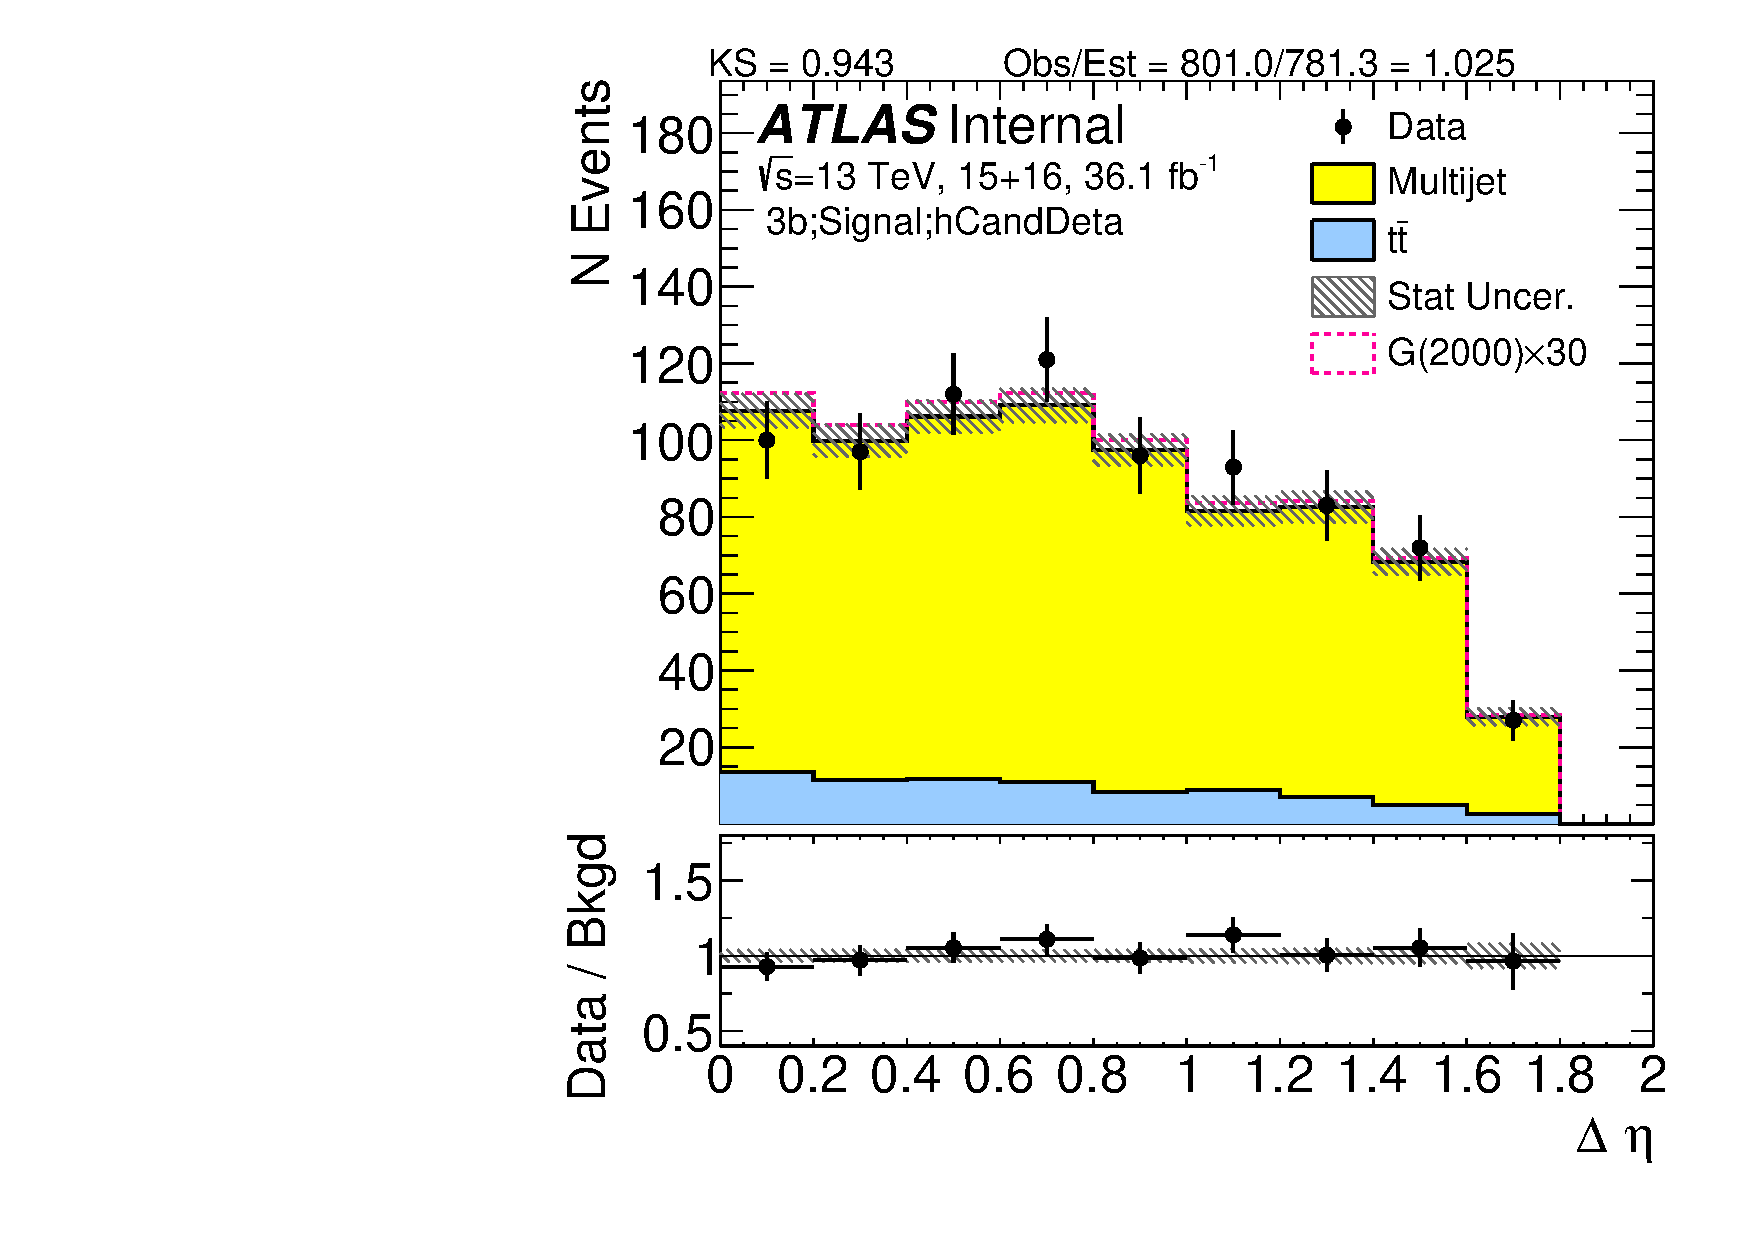
\includegraphics[width=0.31\textwidth,angle=-90]{figures/boosted/Signal/b77_ThreeTag_Signal_hCandDeta.pdf}
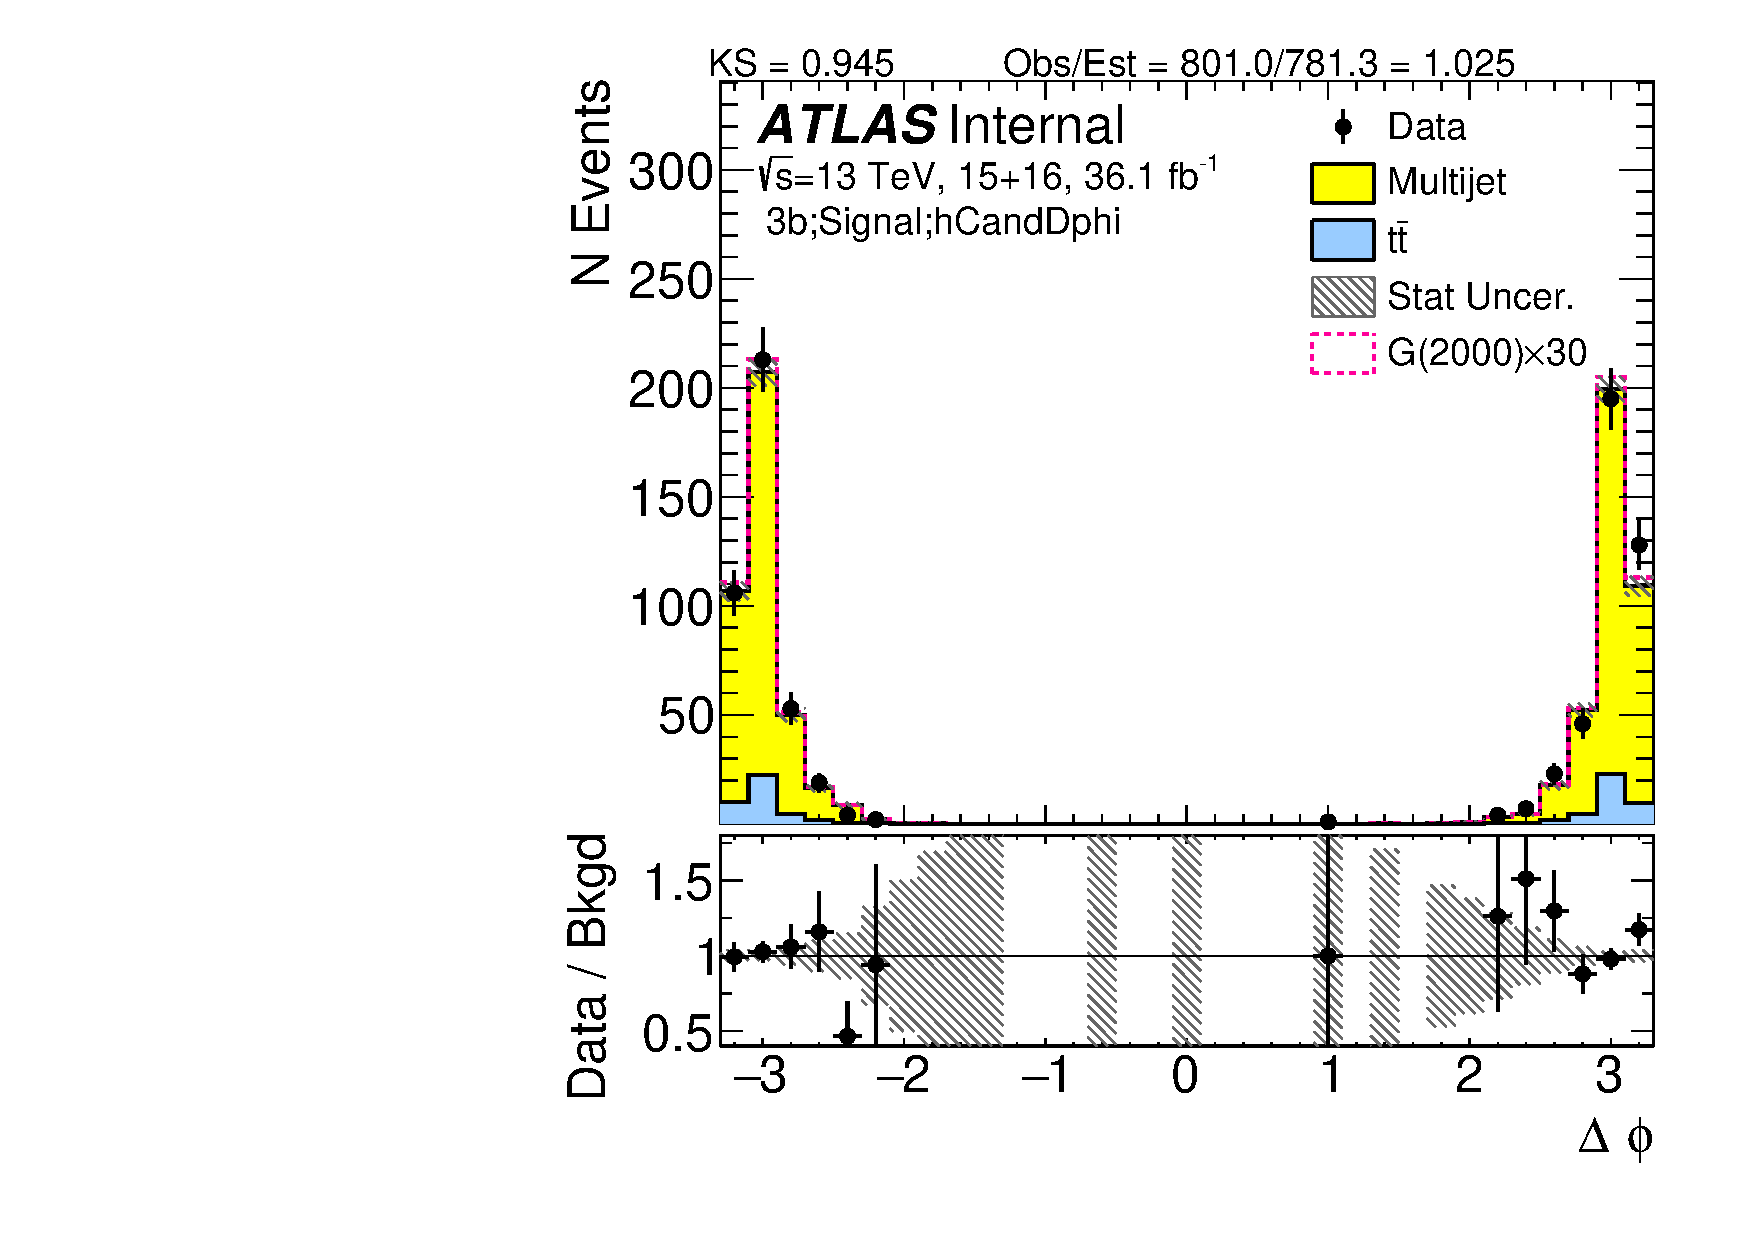
\includegraphics[width=0.31\textwidth,angle=-90]{figures/boosted/Signal/b77_ThreeTag_Signal_hCandDphi.pdf}
  \caption{Kinematics (invariant mass, $\Delta R$, $\Delta \eta$ and $\Delta \phi$) of two large-\R jets in data and prediction in the signal region after requiring 3 $b$-tags.  }
  \label{fig:boosted-3b-signal-ak10-system}
\end{center}
\end{figure*}

\clearpage

\begin{figure*}[htbp!]
\begin{center}
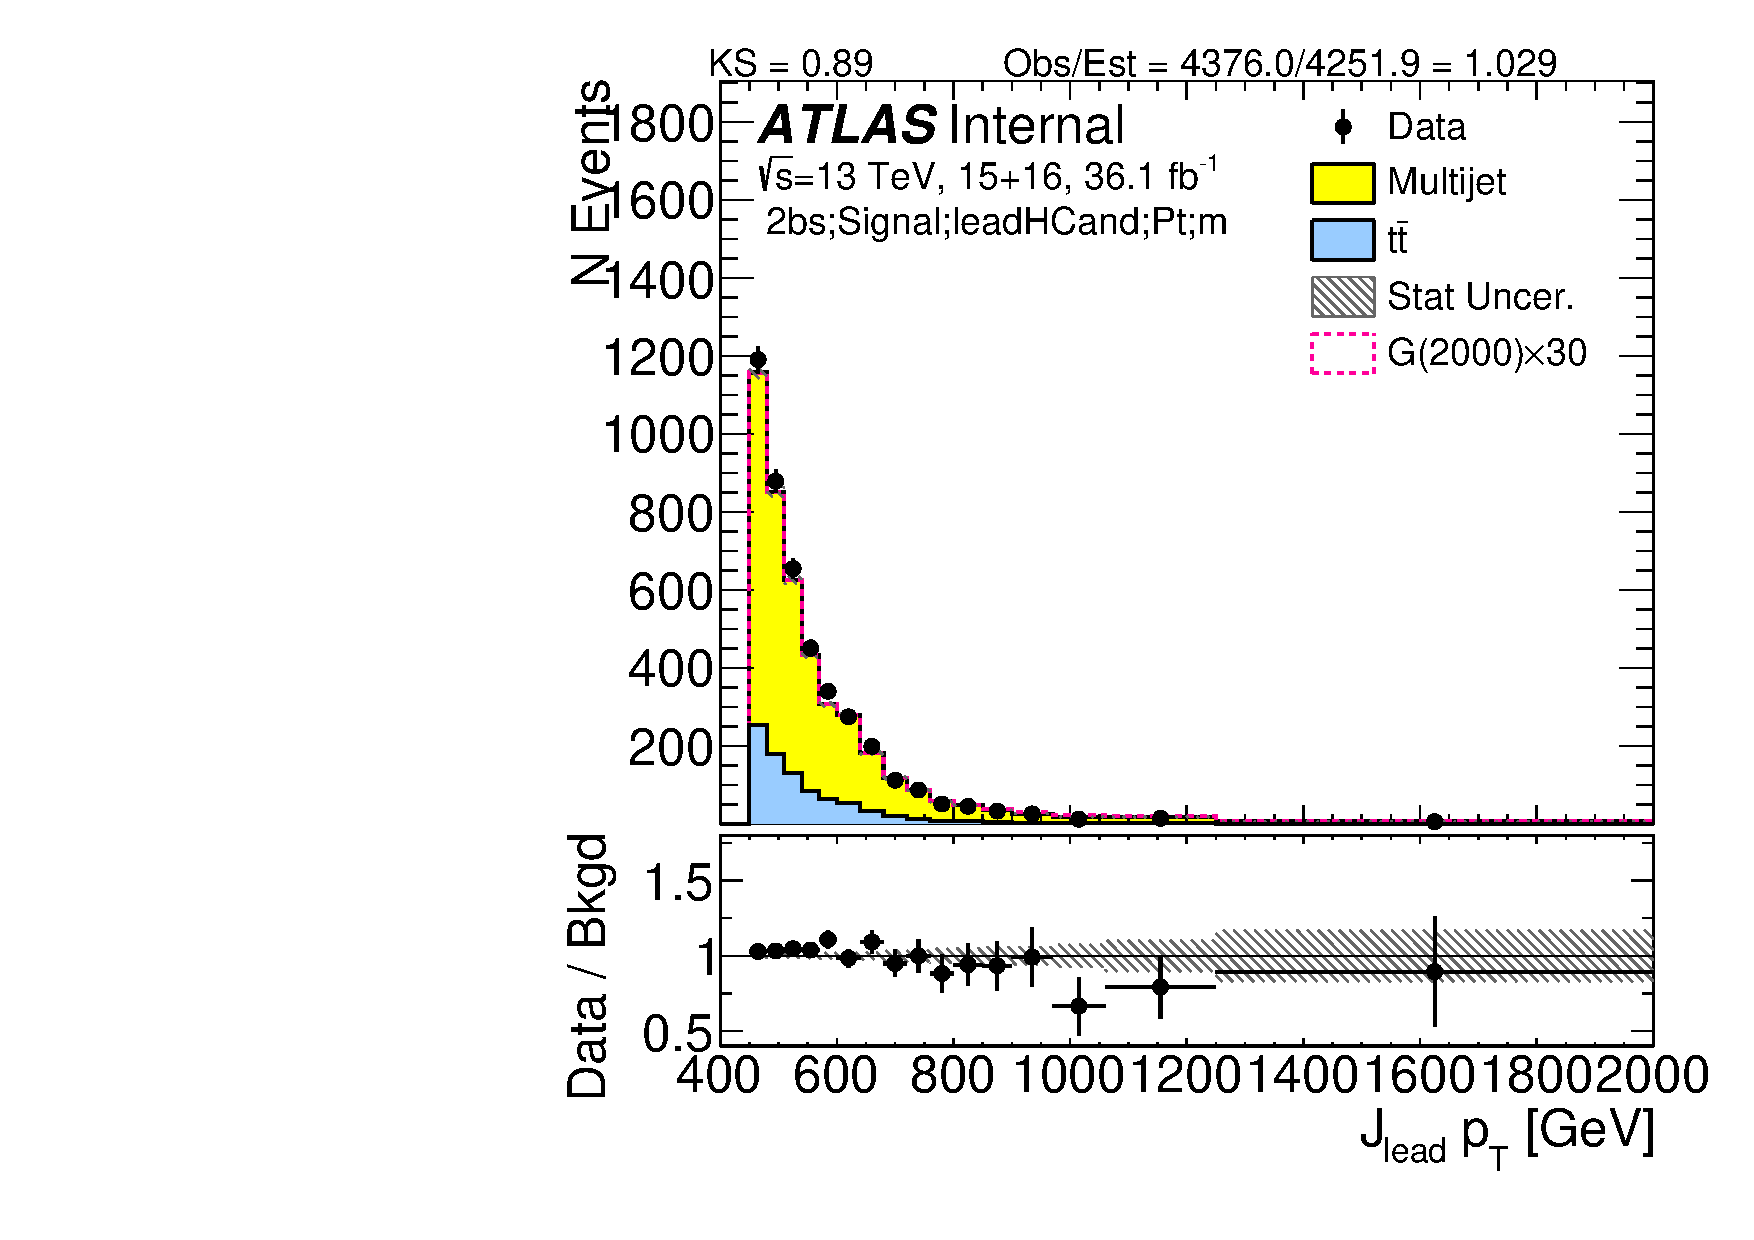
\includegraphics[width=0.31\textwidth,angle=-90]{figures/boosted/Signal/b77_TwoTag_split_Signal_leadHCand_Pt_m.pdf}
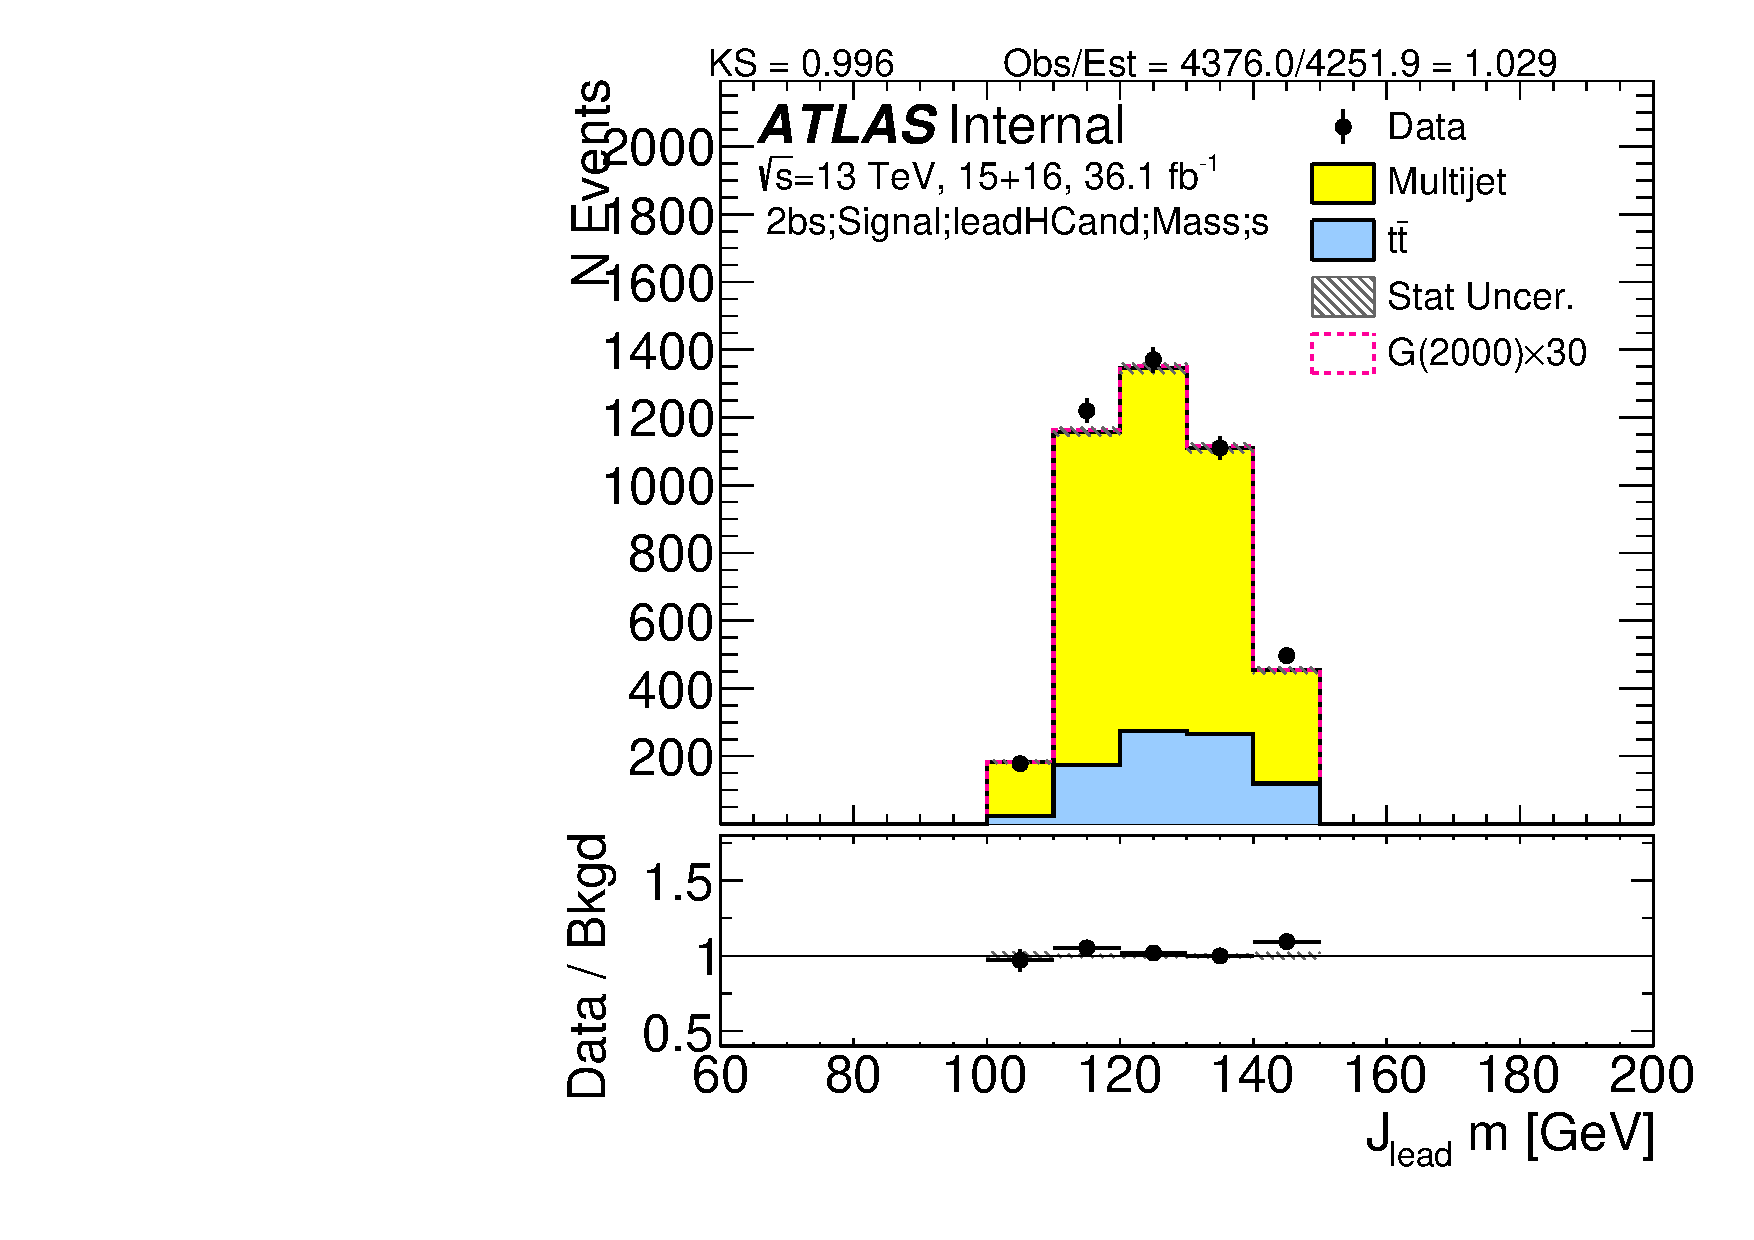
\includegraphics[width=0.31\textwidth,angle=-90]{figures/boosted/Signal/b77_TwoTag_split_Signal_leadHCand_Mass_s.pdf}\\
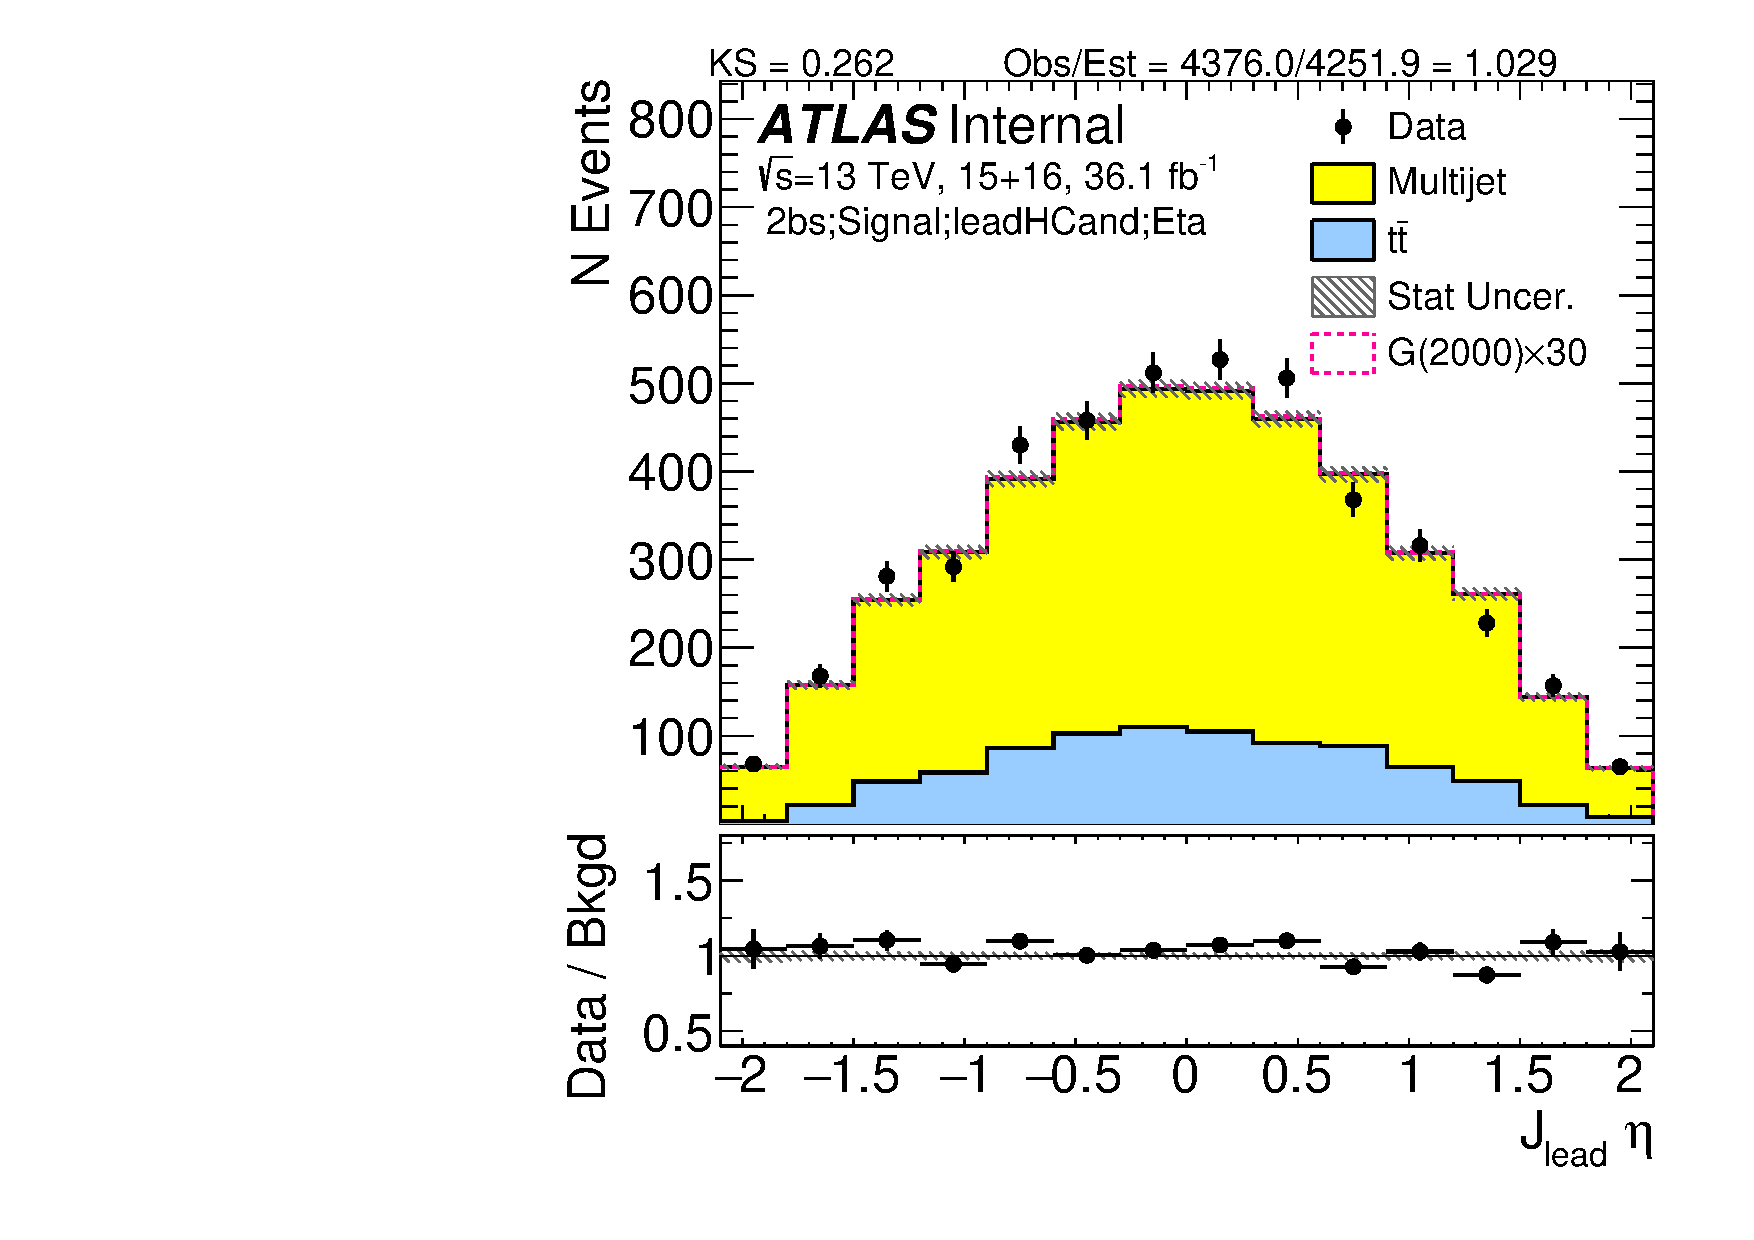
\includegraphics[width=0.31\textwidth,angle=-90]{figures/boosted/Signal/b77_TwoTag_split_Signal_leadHCand_Eta.pdf}
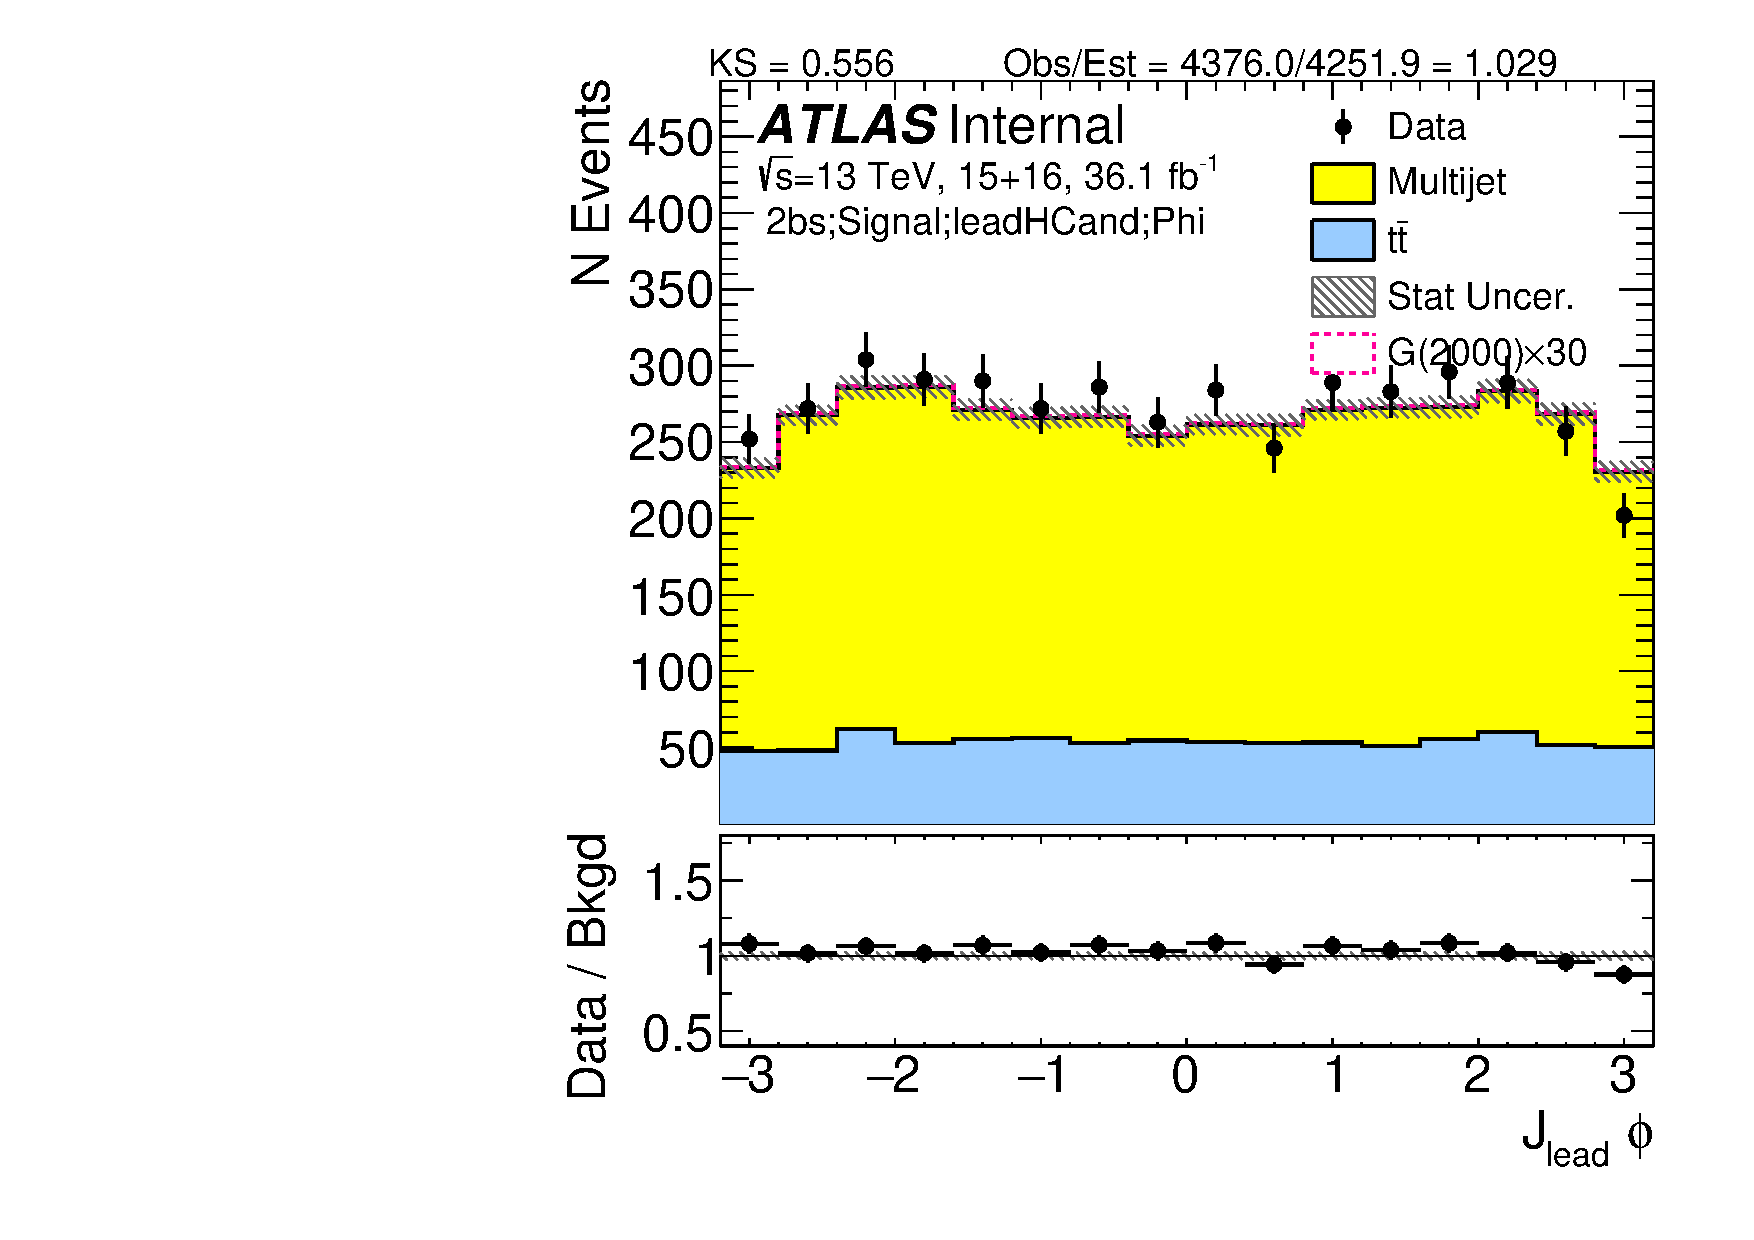
\includegraphics[width=0.31\textwidth,angle=-90]{figures/boosted/Signal/b77_TwoTag_split_Signal_leadHCand_Phi.pdf}
  \caption{Kinematics (\pt~, mass, $\eta$, $\phi$) of the lead large-\R jet in data and prediction in the signal region after requiring 2 $b$-tags split. }
  \label{fig:boosted-2bs-signal-ak10-lead}
\end{center}
\end{figure*}

\begin{figure*}[htbp!]
\begin{center}
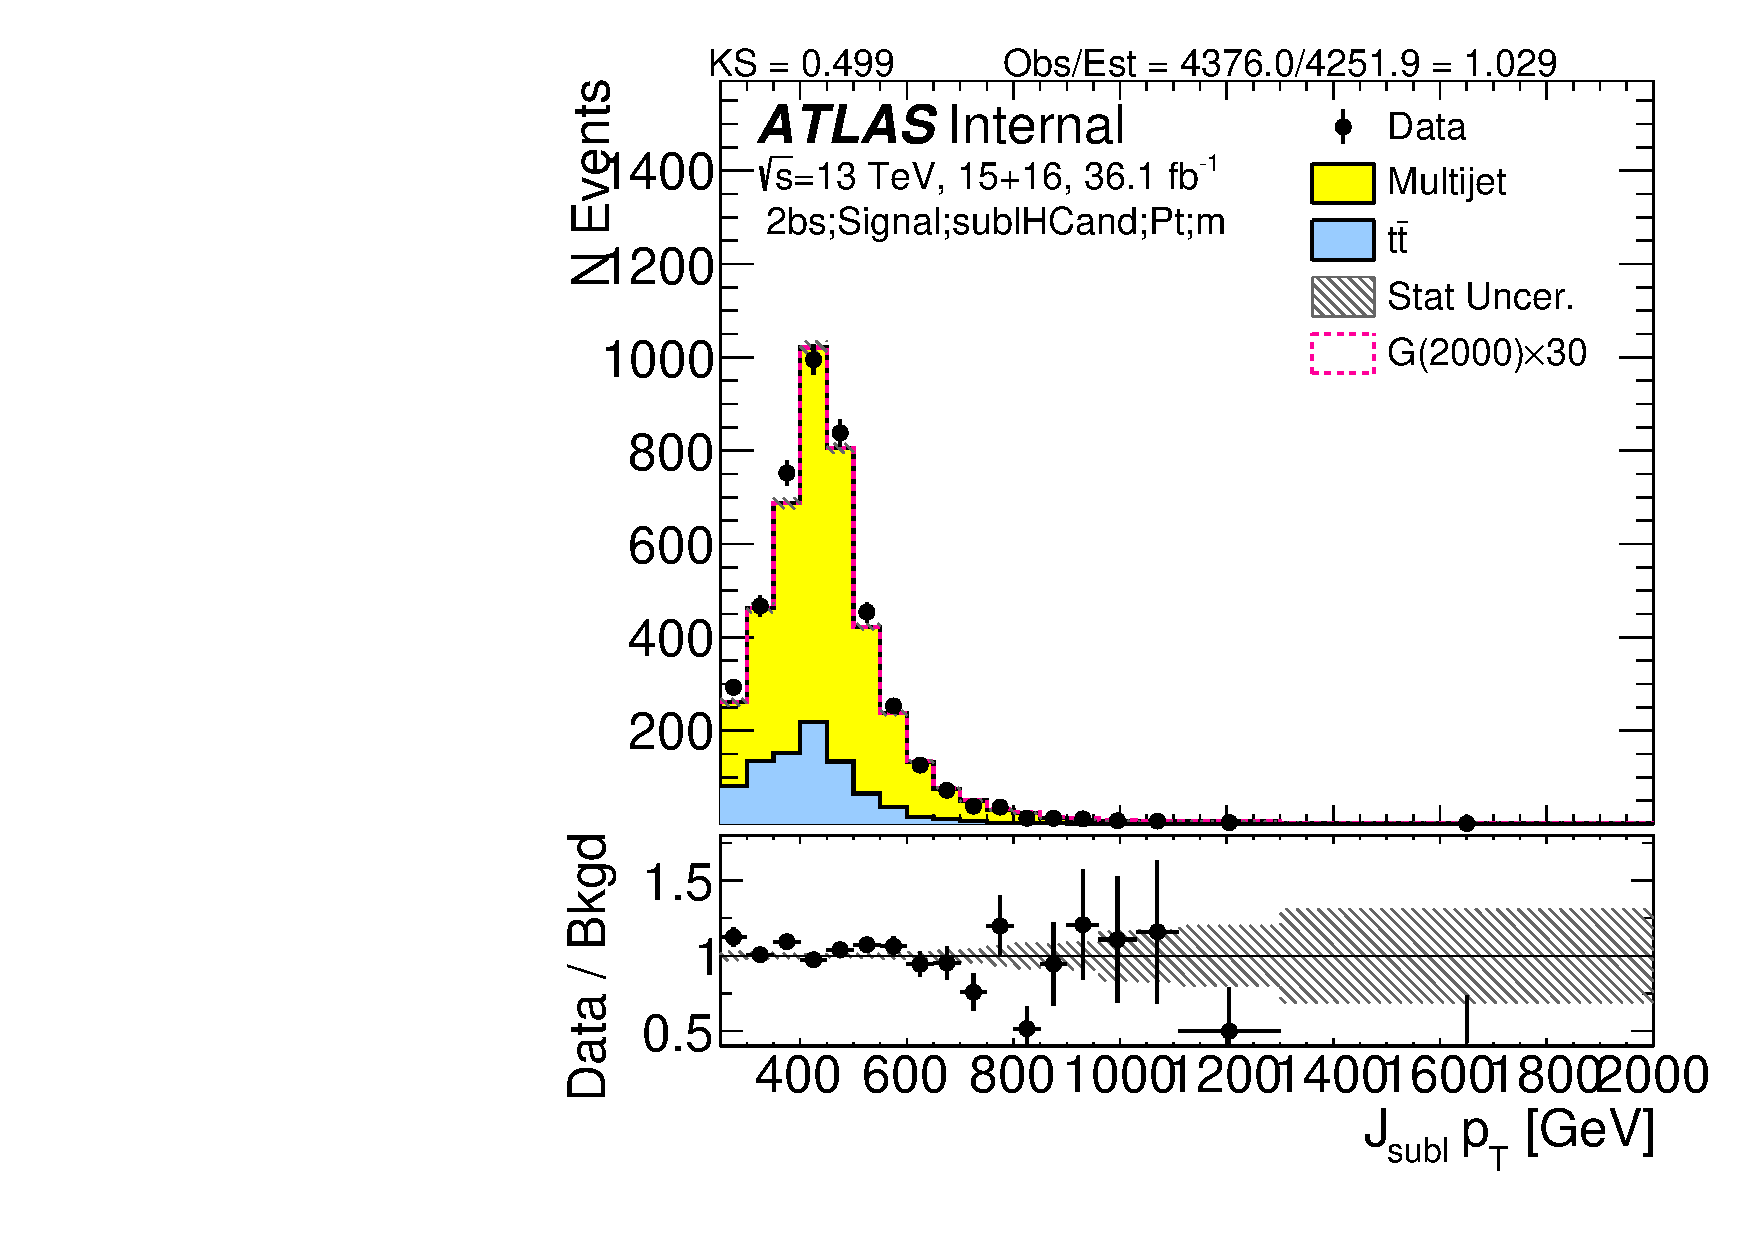
\includegraphics[width=0.31\textwidth,angle=-90]{figures/boosted/Signal/b77_TwoTag_split_Signal_sublHCand_Pt_m.pdf}
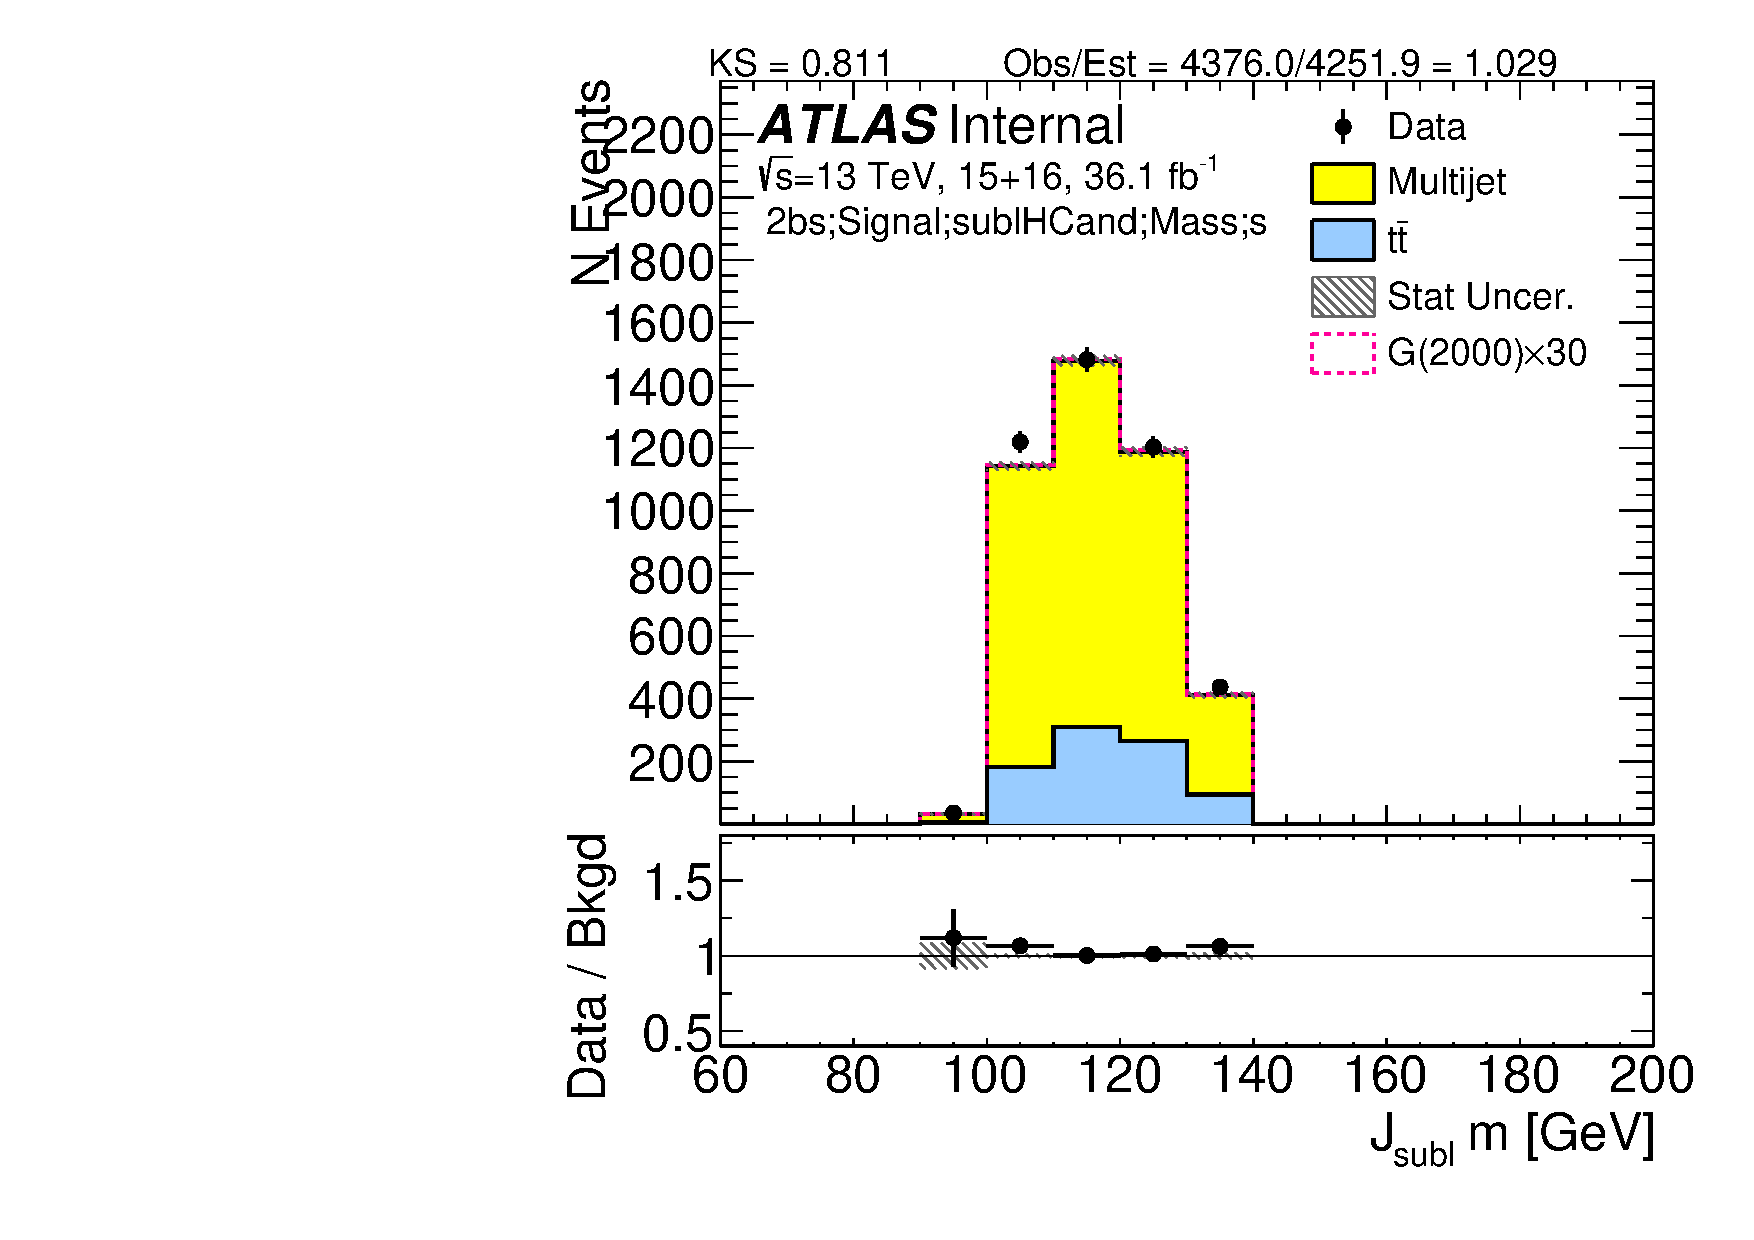
\includegraphics[width=0.31\textwidth,angle=-90]{figures/boosted/Signal/b77_TwoTag_split_Signal_sublHCand_Mass_s.pdf}\\
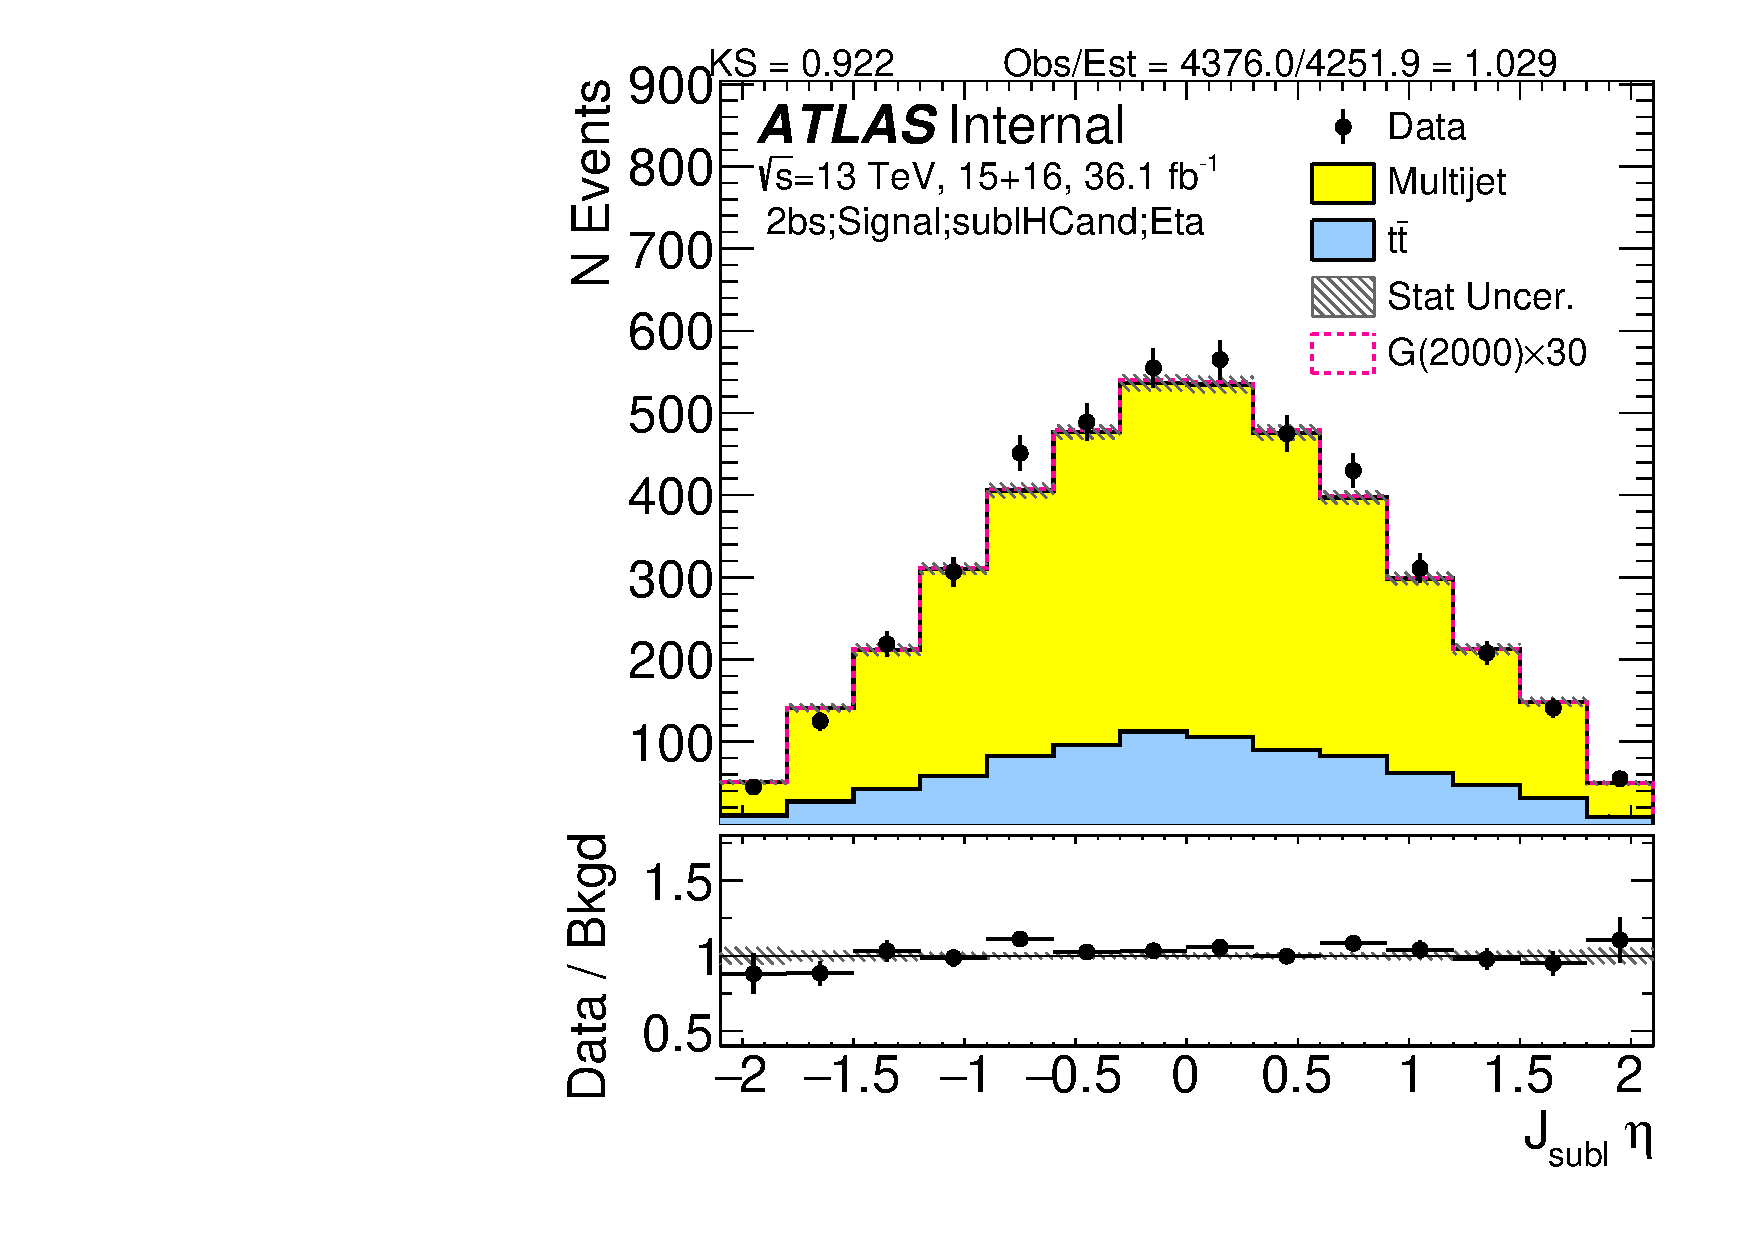
\includegraphics[width=0.31\textwidth,angle=-90]{figures/boosted/Signal/b77_TwoTag_split_Signal_sublHCand_Eta.pdf}
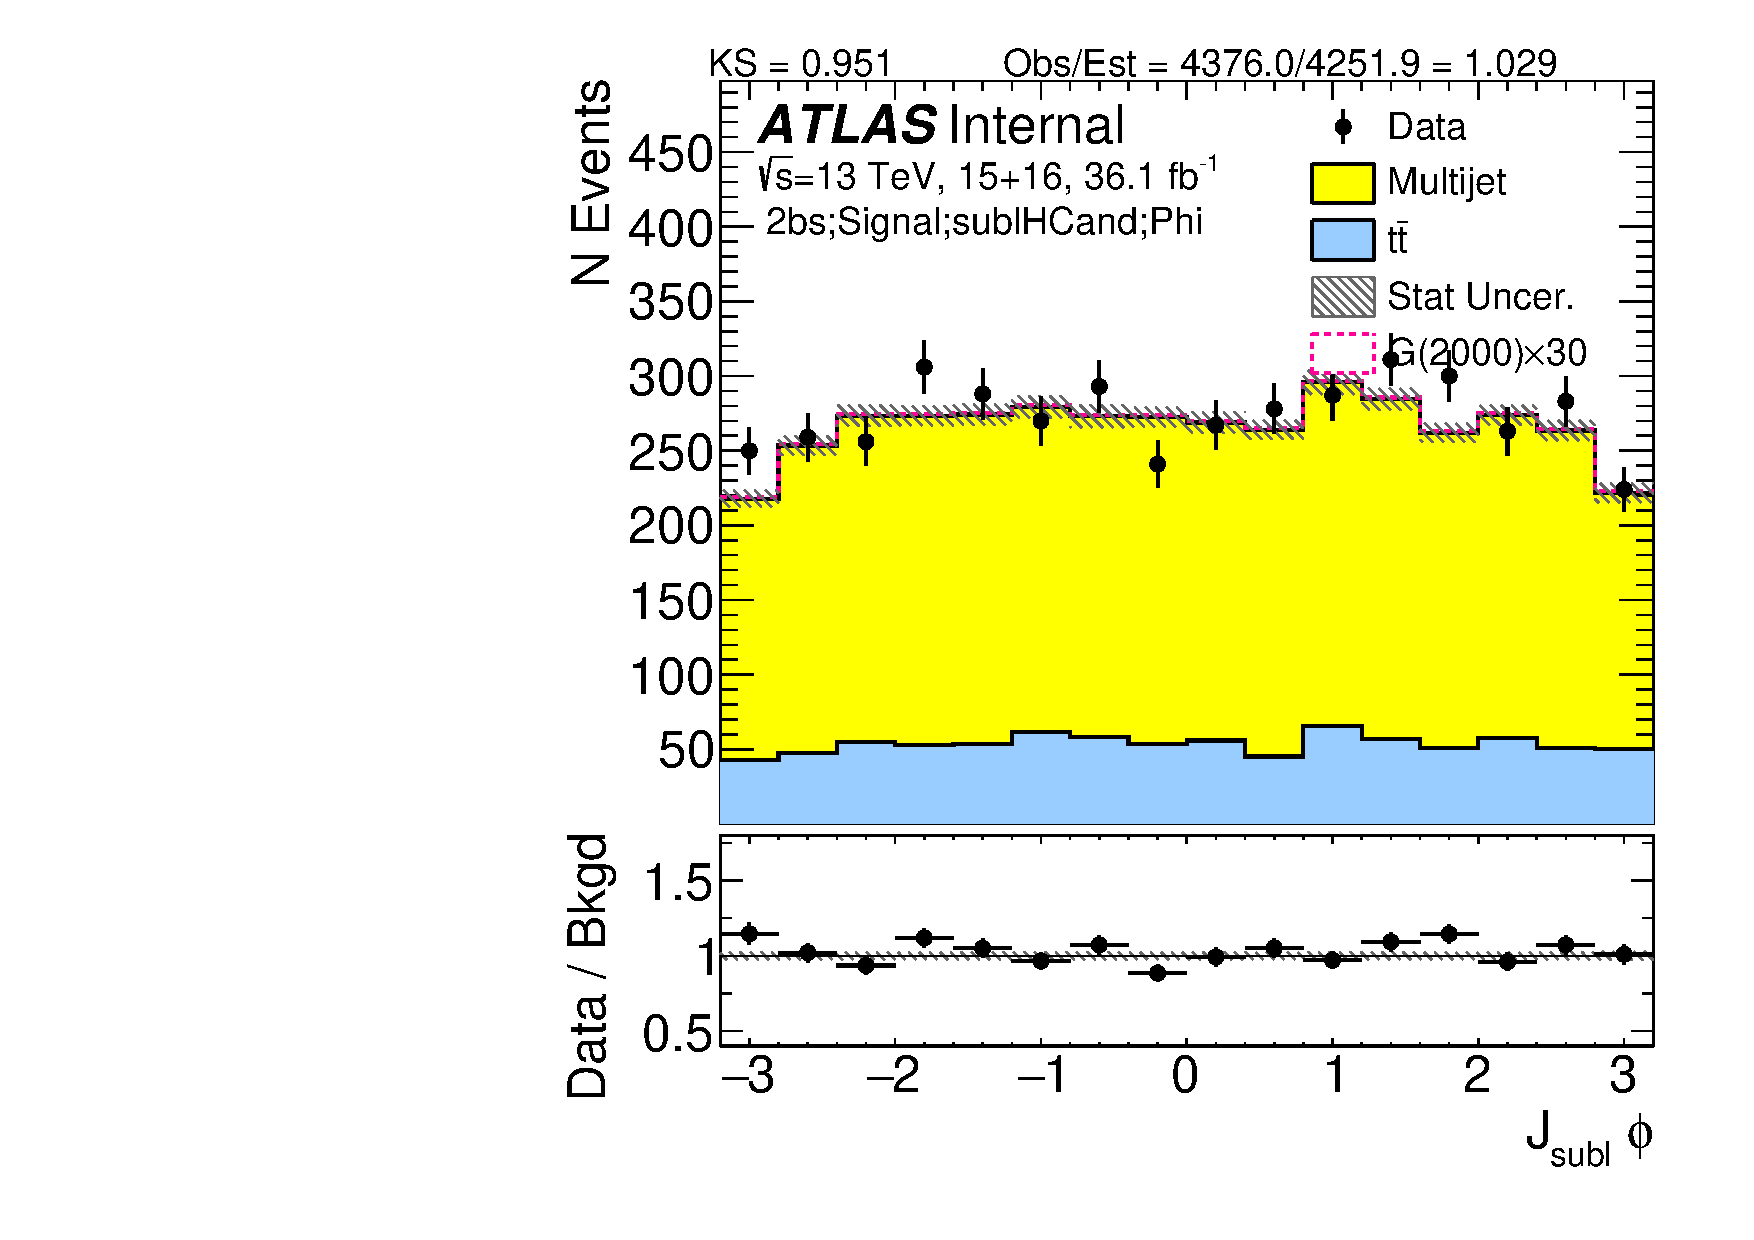
\includegraphics[width=0.31\textwidth,angle=-90]{figures/boosted/Signal/b77_TwoTag_split_Signal_sublHCand_Phi.pdf}
  \caption{Kinematics (\pt~, mass, $\eta$, $\phi$) of the subleading large-\R jet in data and prediction in the signal region after requiring 2 $b$-tags split. }
  \label{fig:boosted-2bs-signal-ak10-subl}
\end{center}
\end{figure*}

\begin{figure*}[htbp!]
\begin{center}
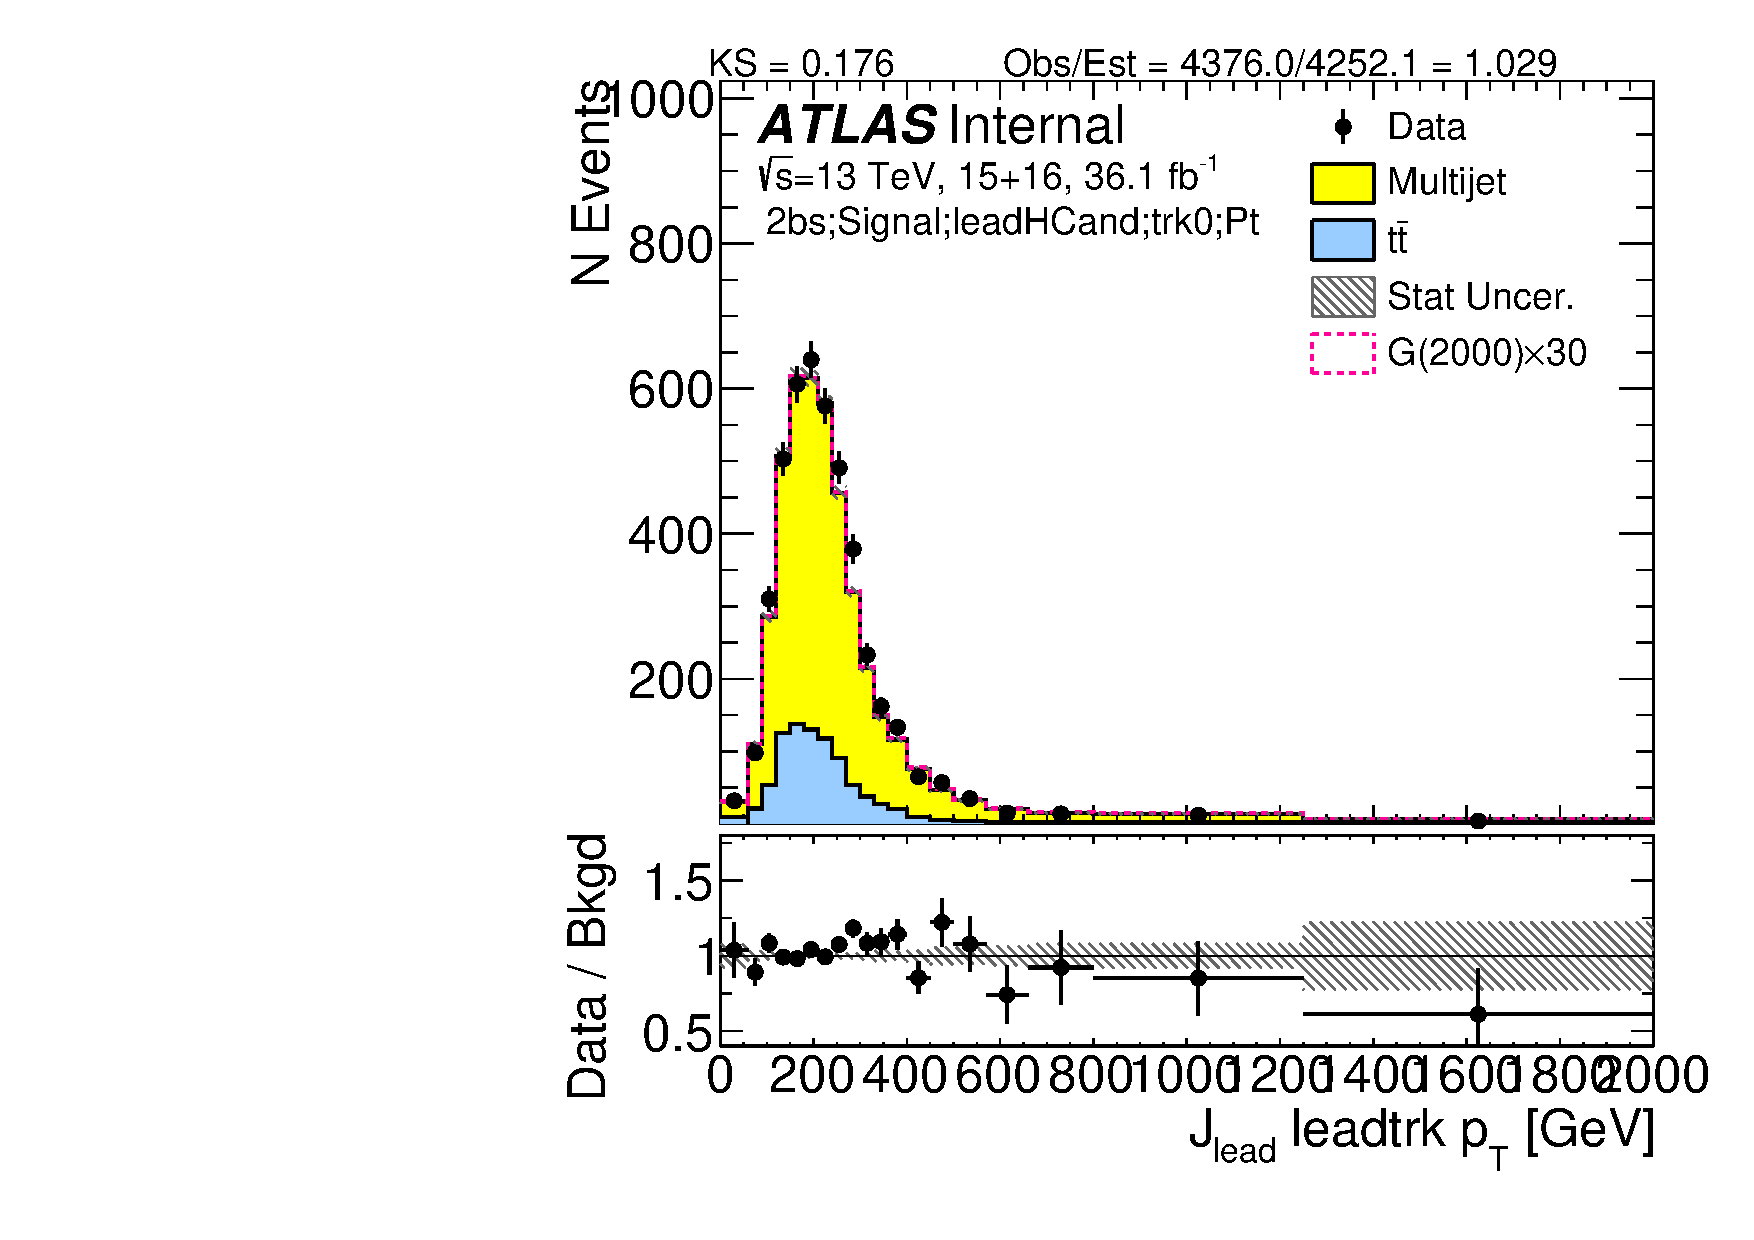
\includegraphics[width=0.31\textwidth,angle=-90]{figures/boosted/Signal/b77_TwoTag_split_Signal_leadHCand_trk0_Pt.pdf}
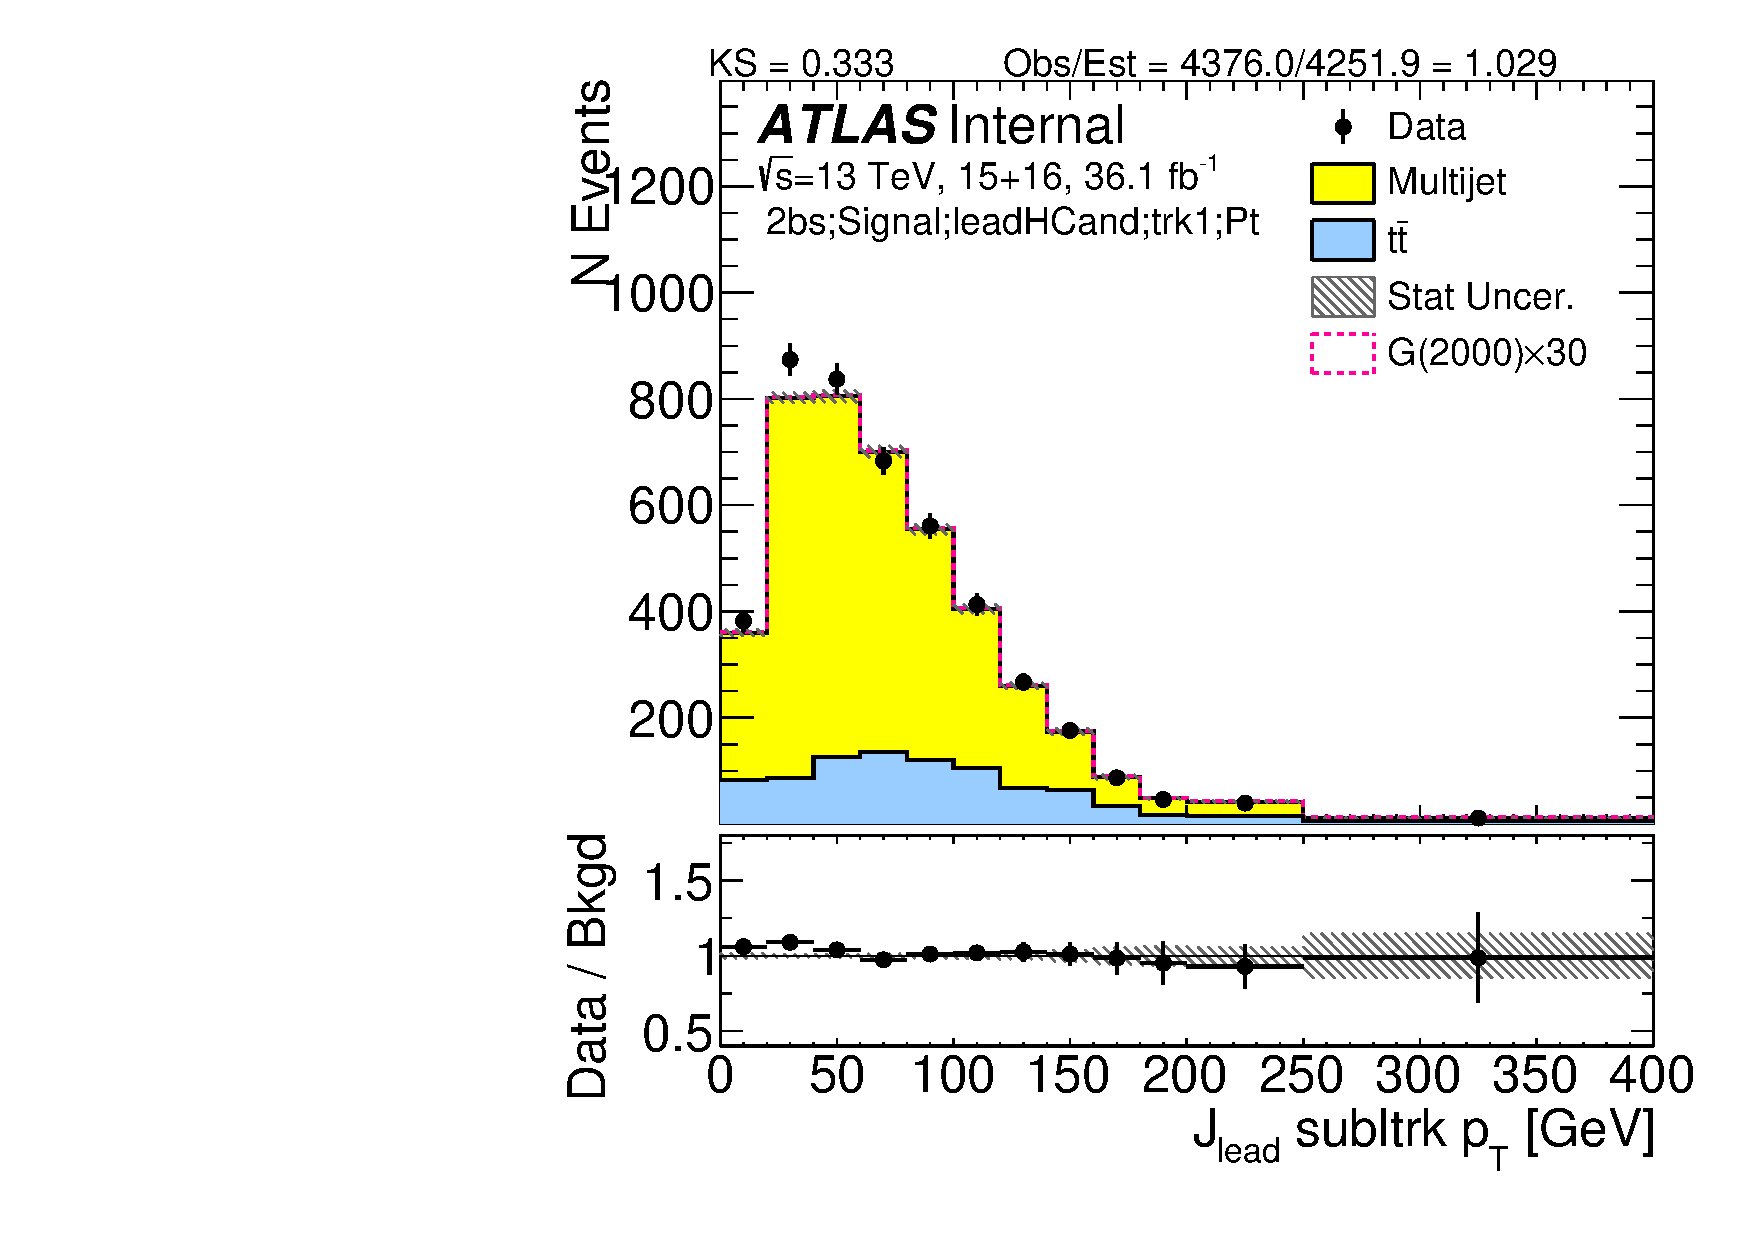
\includegraphics[width=0.31\textwidth,angle=-90]{figures/boosted/Signal/b77_TwoTag_split_Signal_leadHCand_trk1_Pt.pdf}\\
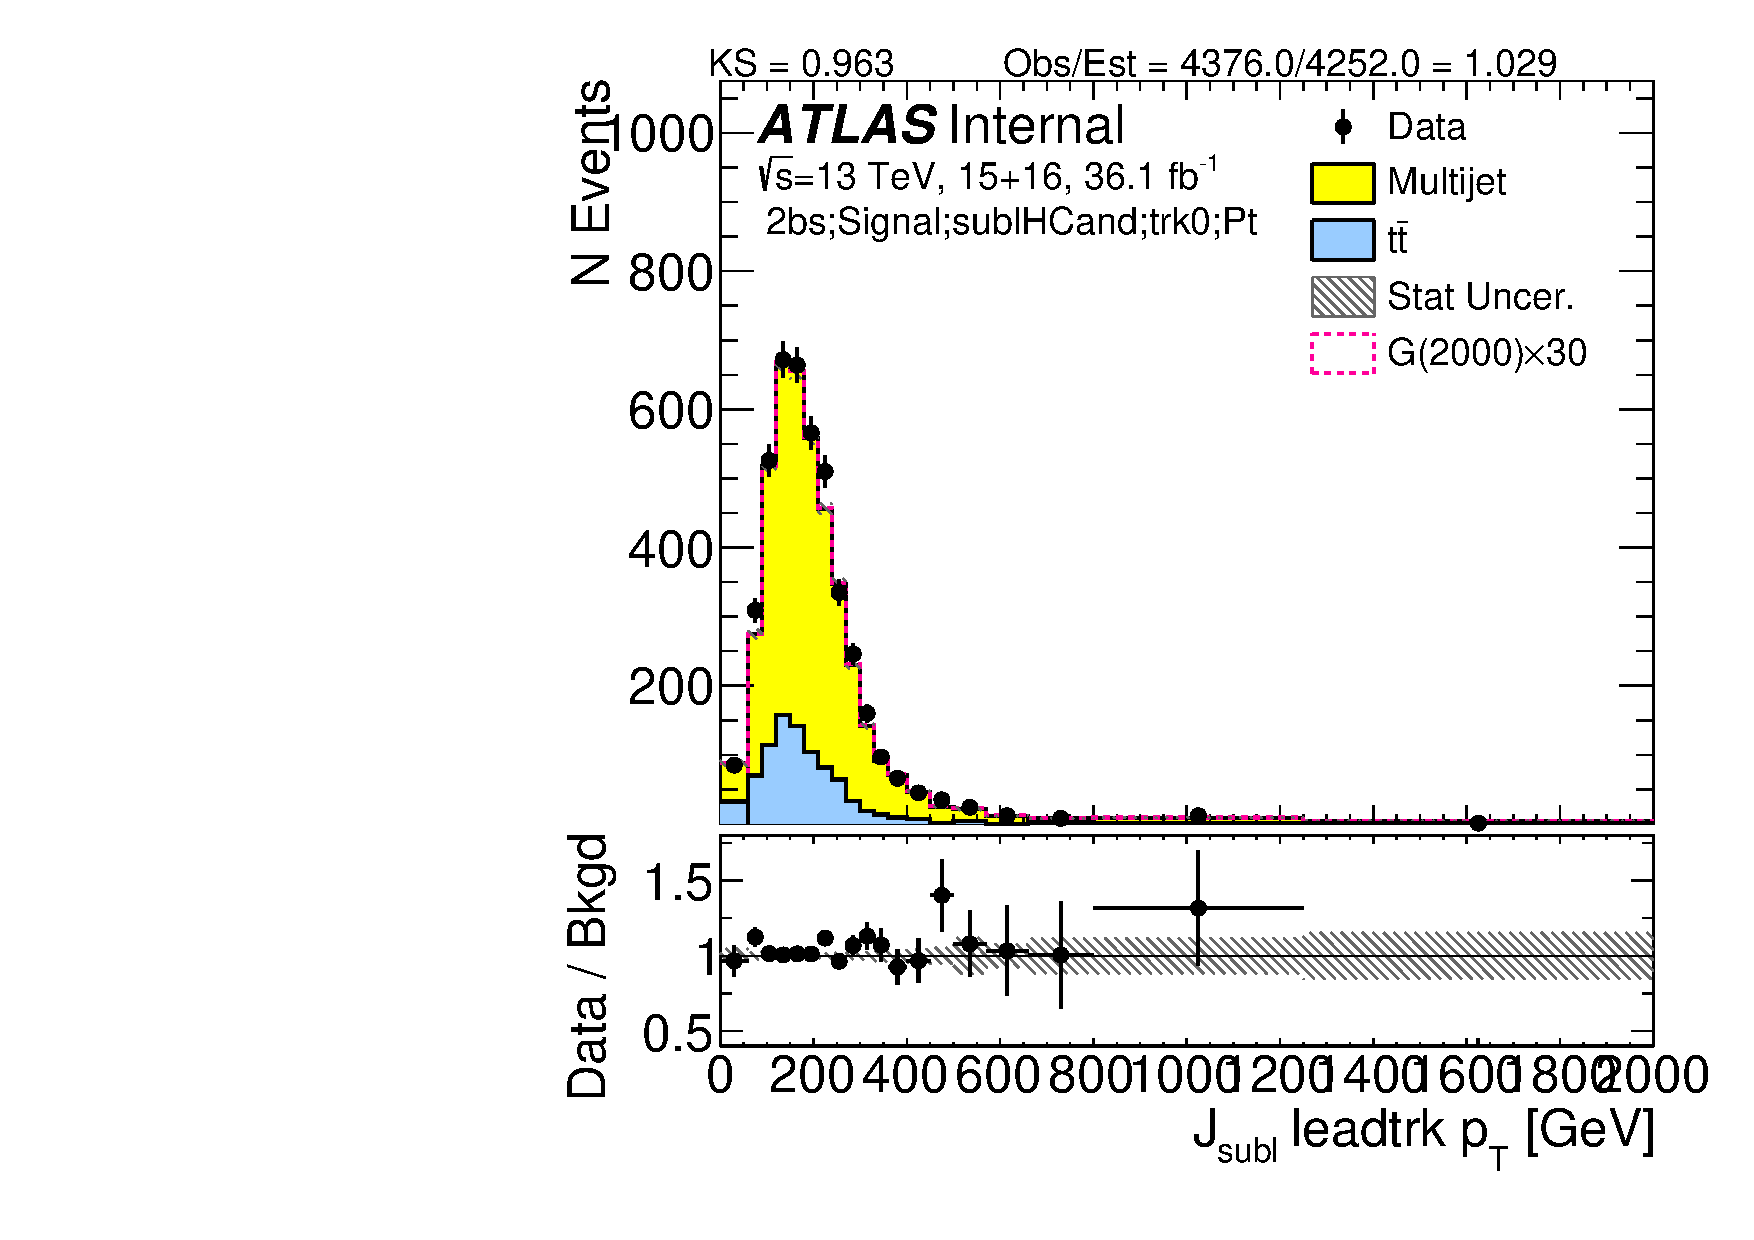
\includegraphics[width=0.31\textwidth,angle=-90]{figures/boosted/Signal/b77_TwoTag_split_Signal_sublHCand_trk0_Pt.pdf}
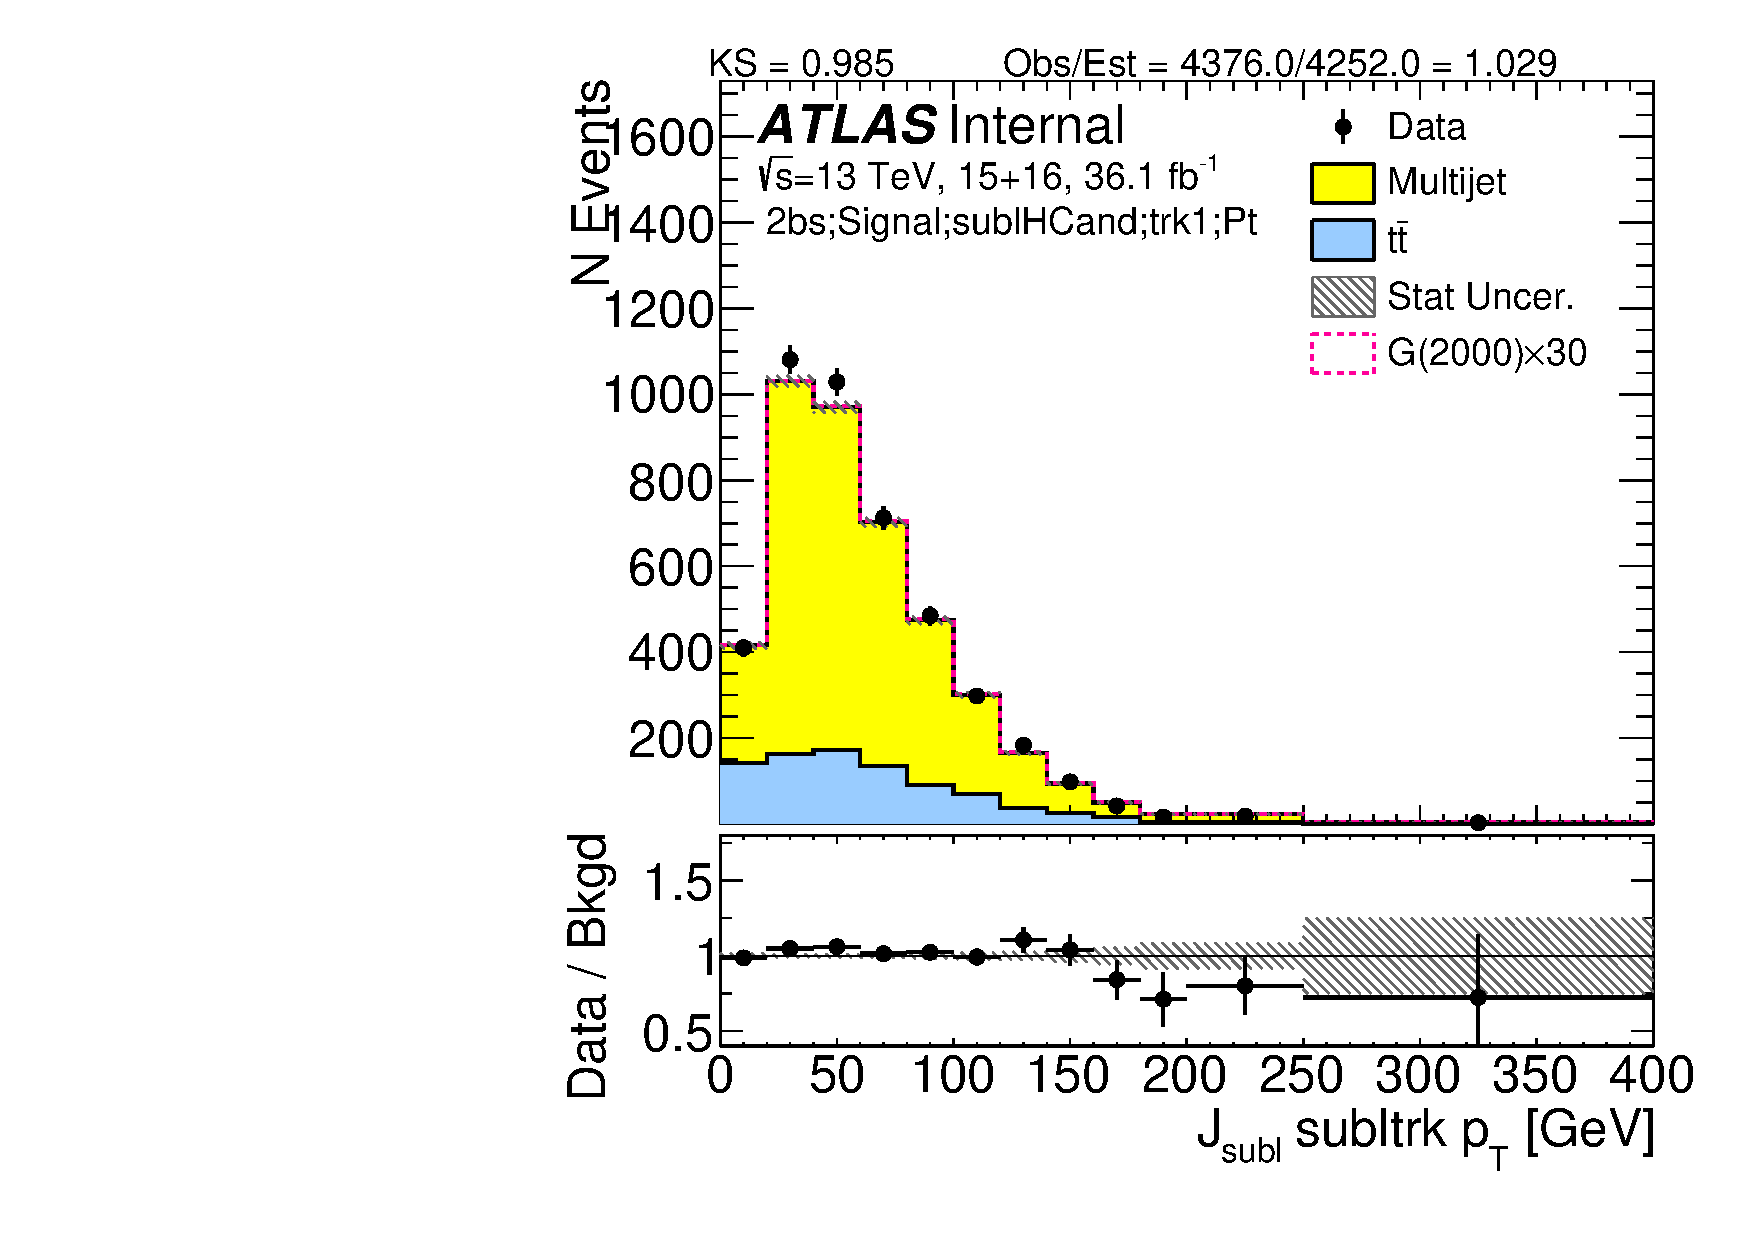
\includegraphics[width=0.31\textwidth,angle=-90]{figures/boosted/Signal/b77_TwoTag_split_Signal_sublHCand_trk1_Pt.pdf}\\
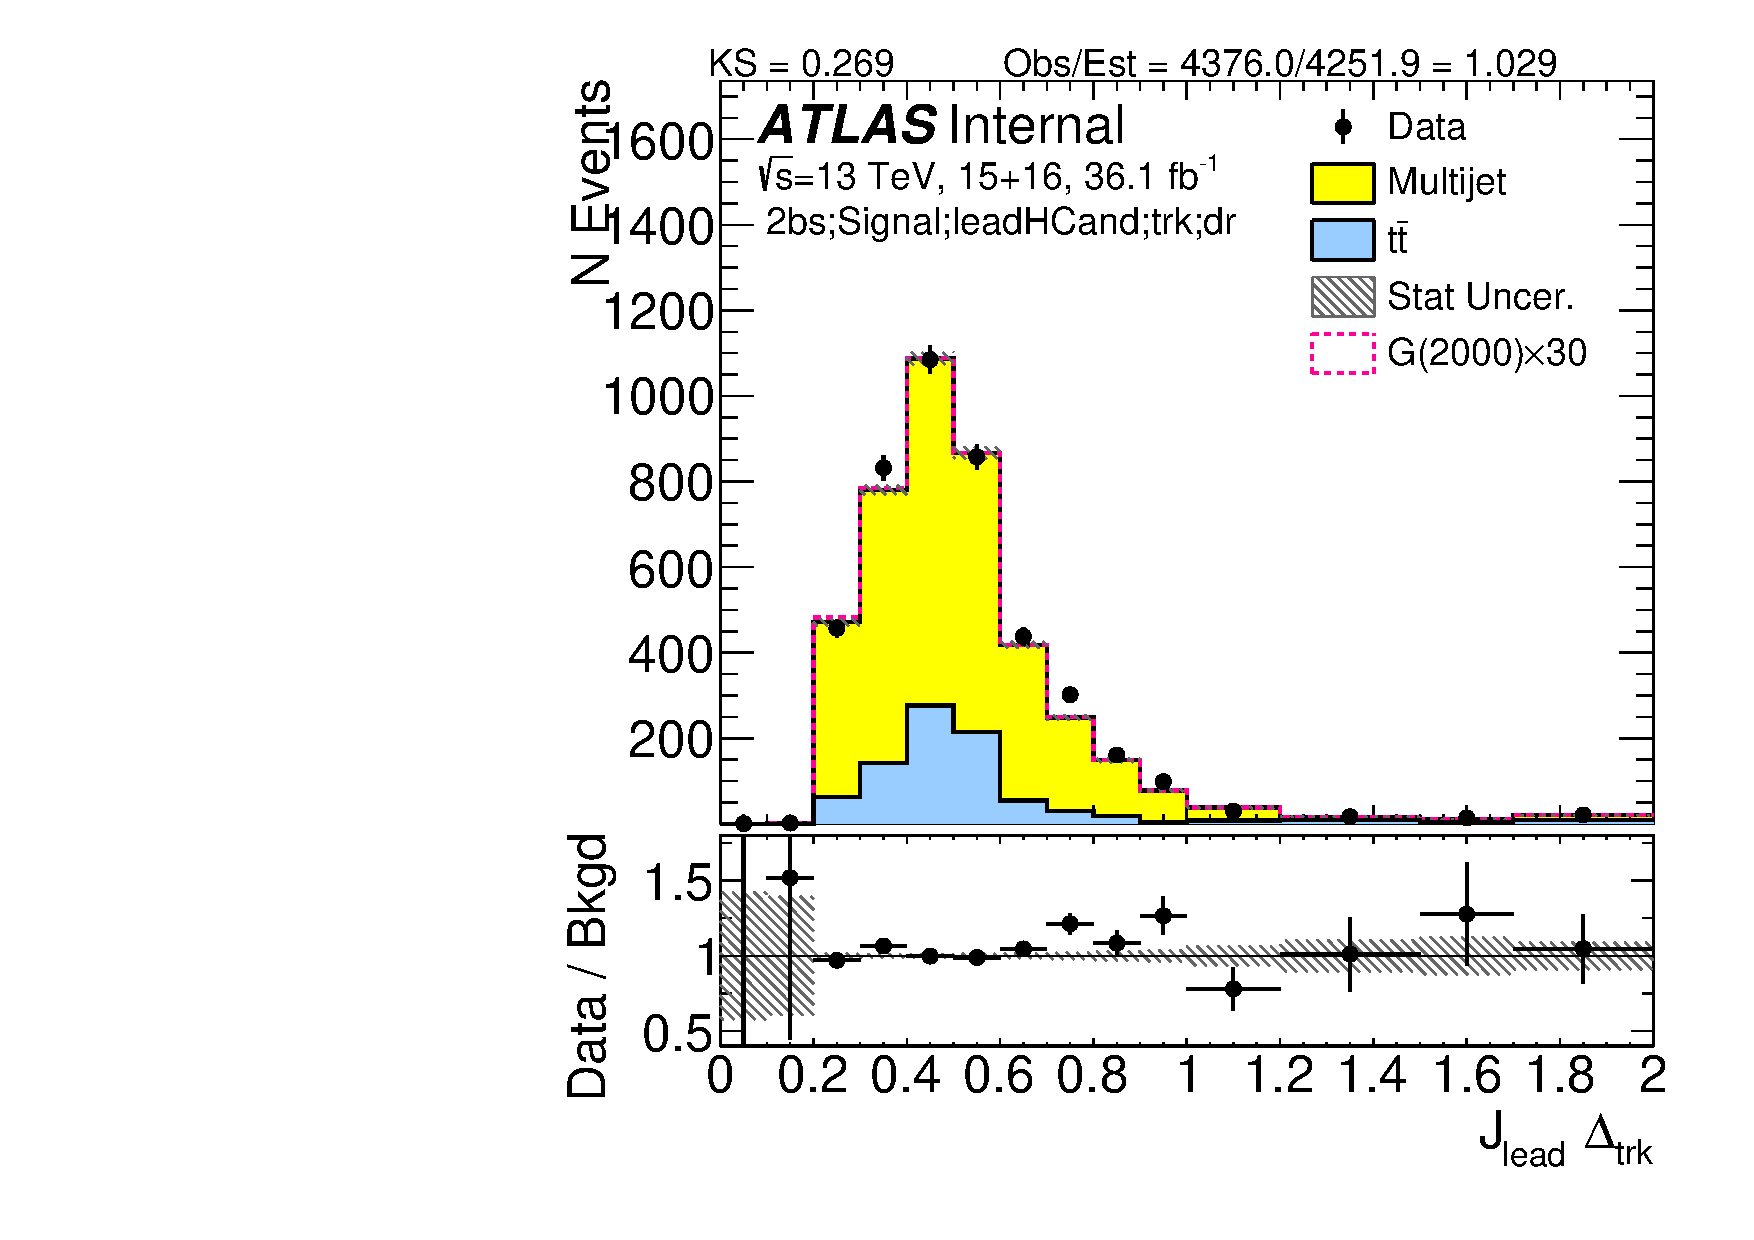
\includegraphics[width=0.31\textwidth,angle=-90]{figures/boosted/Signal/b77_TwoTag_split_Signal_leadHCand_trk_dr.pdf}
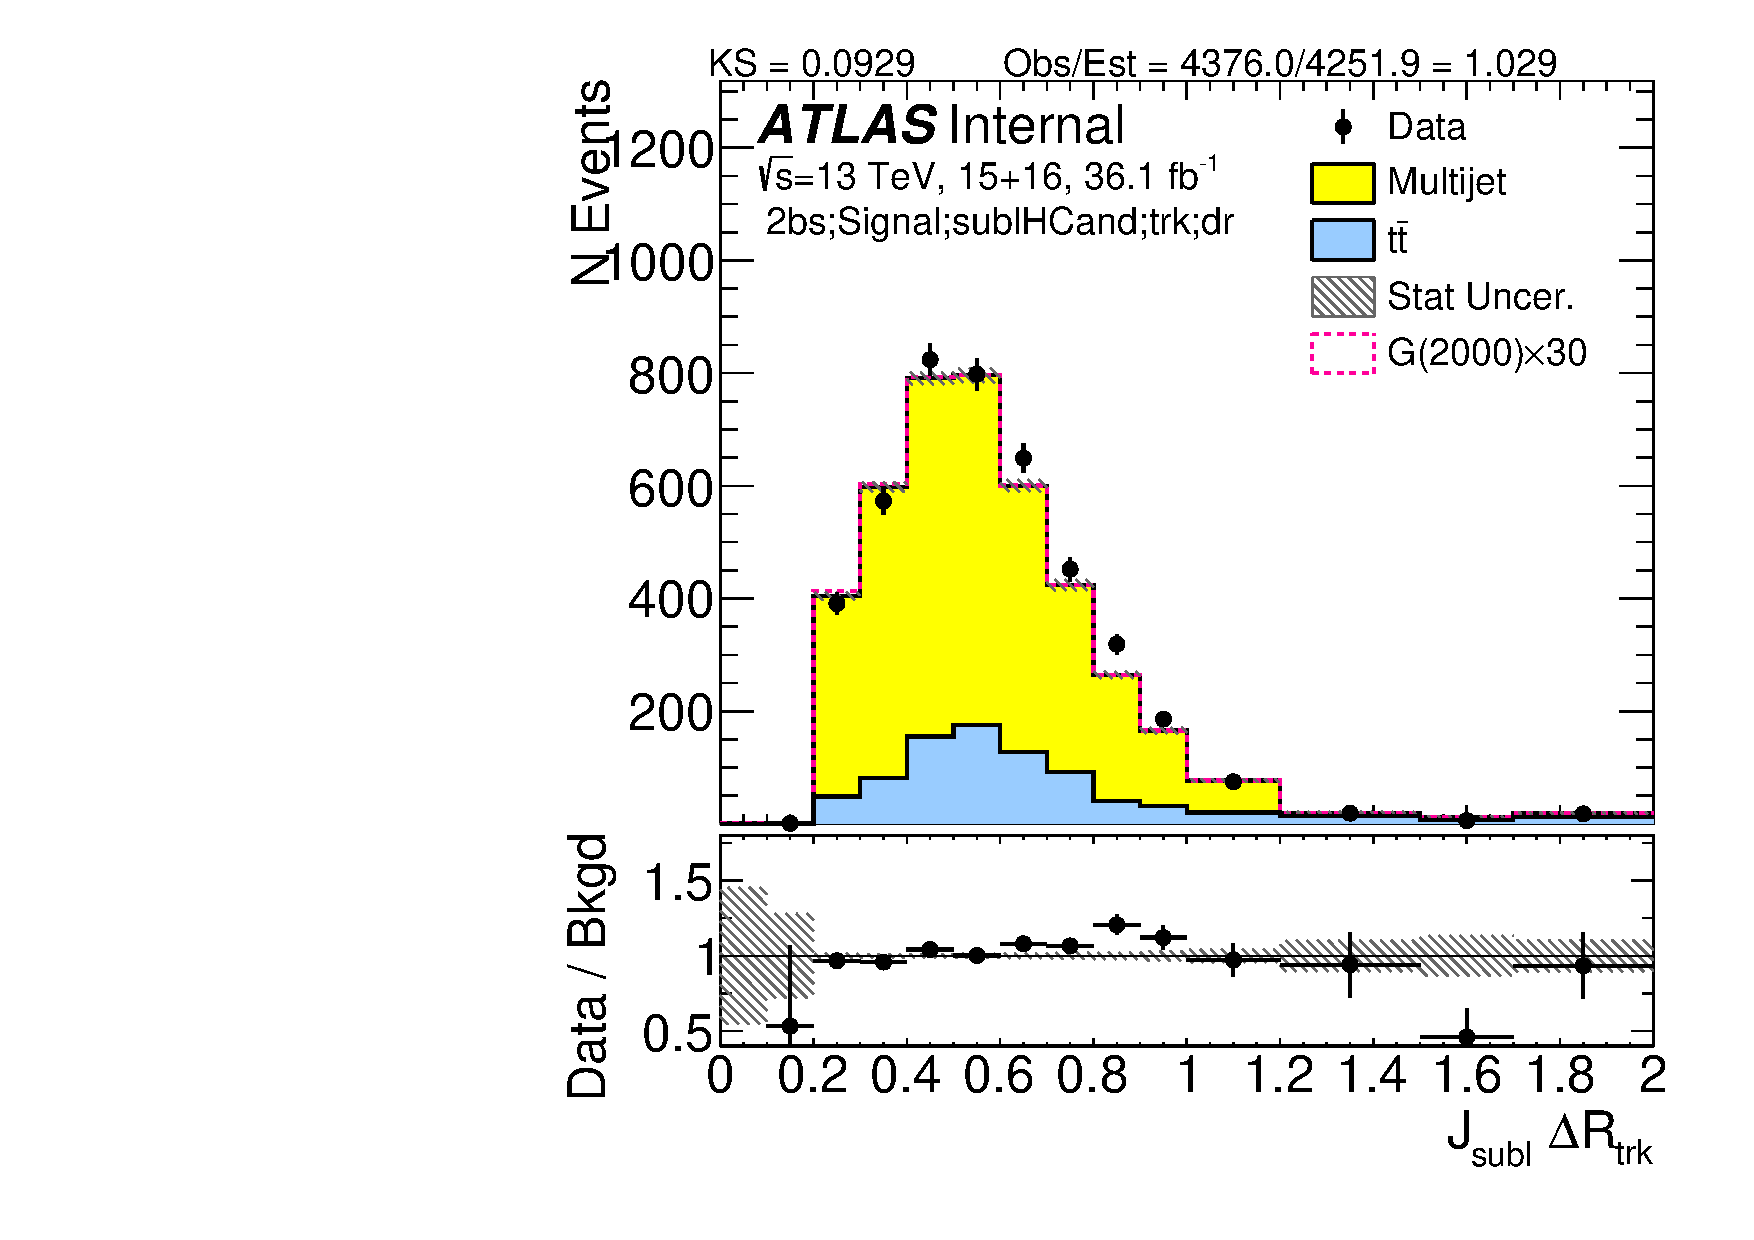
\includegraphics[width=0.31\textwidth,angle=-90]{figures/boosted/Signal/b77_TwoTag_split_Signal_sublHCand_trk_dr.pdf}
  \caption{First two rows show the \pt~ of the lead (left) and sub-lead (right) small-$R$ track jets associated to the lead (first-row) and sub-lead (second-row) large-\R jet in data and prediction in the signal region after requiring 2 $b$-tags split. Third row shows the $\Delta R$ between two leading small-$R$ track-jets associated to the leading (left) and sub-leading (right) large-\R jet.  }
  \label{fig:boosted-2bs-signal-ak2}
\end{center}
\end{figure*}


\begin{figure*}[htbp!]
\begin{center}
\includegraphics[width=0.31\textwidth,angle=-90]{figures/boosted/Signal/b77_TwoTag_split_Signal_mHH_l_1.pdf}
\includegraphics[width=0.31\textwidth,angle=-90]{figures/boosted/Signal/b77_TwoTag_split_Signal_hCandDr.pdf}\\
\includegraphics[width=0.31\textwidth,angle=-90]{figures/boosted/Signal/b77_TwoTag_split_Signal_hCandDeta.pdf}
\includegraphics[width=0.31\textwidth,angle=-90]{figures/boosted/Signal/b77_TwoTag_split_Signal_hCandDphi.pdf}
  \caption{Kinematics (invariant mass, $\Delta R$, $\Delta \eta$ and $\Delta \phi$) of two large-\R jets in data and prediction in the signal region after requiring 2 $b$-tags split.  }
  \label{fig:boosted-2bs-signal-ak10-system}
\end{center}
\end{figure*}


\clearpage
